%% (Master) Thesis template
% Template version used: v1.4
%
% Largely adapted from Adrian Nievergelt's template for the ADPS
% (lecture notes) project.


%% We use the memoir class because it offers a many easy to use features.
\documentclass[11pt,a4paper,titlepage]{memoir}

%% Packages
%% ========

%% LaTeX Font encoding -- DO NOT CHANGE
\usepackage[OT1]{fontenc}

%% Babel provides support for languages.  'english' uses British
%% English hyphenation and text snippets like "Figure" and
%% "Theorem". Use the option 'ngerman' if your document is in German.
%% Use 'american' for American English.  Note that if you change this,
%% the next LaTeX run may show spurious errors.  Simply run it again.
%% If they persist, remove the .aux file and try again.
\usepackage[english]{babel}

%% Input encoding 'utf8'. In some cases you might need 'utf8x' for
%% extra symbols. Not all editors, especially on Windows, are UTF-8
%% capable, so you may want to use 'latin1' instead.
\usepackage[utf8]{inputenc}

\usepackage{dirtree}

%% This changes default fonts for both text and math mode to use Herman Zapfs
%% excellent Palatino font.  Do not change this.
\usepackage[sc]{mathpazo}

%% The AMS-LaTeX extensions for mathematical typesetting.  Do not
%% remove.
\usepackage{amsmath,amssymb,amsfonts,mathrsfs}

%% NTheorem is a reimplementation of the AMS Theorem package. This
%% will allow us to typeset theorems like examples, proofs and
%% similar.  Do not remove.
%% NOTE: Must be loaded AFTER amsmath, or the \qed placement will
%% break
\usepackage[amsmath,thmmarks]{ntheorem}

%% LaTeX' own graphics handling
\usepackage{graphicx}

%% We unfortunately need this for the Rules chapter.  Remove it
%% afterwards; or at least NEVER use its underlining features.
\usepackage{soul}

%% This allows you to add .pdf files. It is used to add the
%% declaration of originality.
\usepackage{pdfpages}

\usepackage{booktabs}
\newcommand{\ra}[1]{\renewcommand{\arraystretch}{#1}}

\usepackage{subcaption}
\usepackage{pdflscape}
%% Some more packages that you may want to use.  Have a look at the
%% file, and consult the package docs for each.
%% See the TeXed file for more explanations

%% [OPT] Multi-rowed cells in tabulars
%\usepackage{multirow}

%% [REC] Intelligent cross reference package. This allows for nice
%% combined references that include the reference and a hint to where
%% to look for it.
\usepackage{varioref}

%% [OPT] Easily changeable quotes with \enquote{Text}
%\usepackage[german=swiss]{csquotes}

%% [REC] Format dates and time depending on locale
\usepackage{datetime}

%% [OPT] Provides a \cancel{} command to stroke through mathematics.
%\usepackage{cancel}

%% [NEED] This allows for additional typesetting tools in mathmode.
%% See its excellent documentation.
\usepackage{mathtools}

%% [ADV] Conditional commands
%\usepackage{ifthen}

%% [OPT] Manual large braces or other delimiters.
%\usepackage{bigdelim, bigstrut}

%% [REC] Alternate vector arrows. Use the command \vv{} to get scaled
%% vector arrows.
\usepackage[h]{esvect}

%% [NEED] Some extensions to tabulars and array environments.
\usepackage{array}

%% [OPT] Postscript support via pstricks graphics package. Very
%% diverse applications.
%\usepackage{pstricks,pst-all}

%% [?] This seems to allow us to define some additional counters.
%\usepackage{etex}

%% [ADV] XY-Pic to typeset some matrix-style graphics
%\usepackage[all]{xy}

%% [OPT] This is needed to generate an index at the end of the
%% document.
%\usepackage{makeidx}

%% [OPT] Fancy package for source code listings.  The template text
%% needs it for some LaTeX snippets; remove/adapt the \lstset when you
%% remove the template content.
\usepackage{listings}
\lstset{language=TeX,basicstyle={\normalfont\ttfamily}}

%% [REC] Fancy character protrusion.  Must be loaded after all fonts.
\usepackage[activate]{pdfcprot}

%% [REC] Nicer tables.  Read the excellent documentation.
\usepackage{booktabs}


%% Our layout configuration.  DO NOT CHANGE.
%% Memoir layout setup

%% NOTE: You are strongly advised not to change any of them unless you
%% know what you are doing.  These settings strongly interact in the
%% final look of the document.

% Dependencies
\usepackage{ETHlogo}

% Turn extra space before chapter headings off.
\setlength{\beforechapskip}{0pt}

\nonzeroparskip
\parindent=0pt
\defaultlists

% Chapter style redefinition
\makeatletter

\if@twoside
  \pagestyle{Ruled}
  \copypagestyle{chapter}{Ruled}
\else
  \pagestyle{ruled}
  \copypagestyle{chapter}{ruled}
\fi
\makeoddhead{chapter}{}{}{}
\makeevenhead{chapter}{}{}{}
\makeheadrule{chapter}{\textwidth}{0pt}
\copypagestyle{abstract}{empty}

\makechapterstyle{bianchimod}{%
  \chapterstyle{default}
  \renewcommand*{\chapnamefont}{\normalfont\Large\sffamily}
  \renewcommand*{\chapnumfont}{\normalfont\Large\sffamily}
  \renewcommand*{\printchaptername}{%
    \chapnamefont\centering\@chapapp}
  \renewcommand*{\printchapternum}{\chapnumfont {\thechapter}}
  \renewcommand*{\chaptitlefont}{\normalfont\huge\sffamily}
  \renewcommand*{\printchaptertitle}[1]{%
    \hrule\vskip\onelineskip \centering \chaptitlefont\textbf{\vphantom{gyM}##1}\par}
  \renewcommand*{\afterchaptertitle}{\vskip\onelineskip \hrule\vskip
    \afterchapskip}
  \renewcommand*{\printchapternonum}{%
    \vphantom{\chapnumfont {9}}\afterchapternum}}

% Use the newly defined style
\chapterstyle{bianchimod}

\setsecheadstyle{\Large\bfseries\sffamily}
\setsubsecheadstyle{\large\bfseries\sffamily}
\setsubsubsecheadstyle{\bfseries\sffamily}
\setparaheadstyle{\normalsize\bfseries\sffamily}
\setsubparaheadstyle{\normalsize\itshape\sffamily}
\setsubparaindent{0pt}

% Set captions to a more separated style for clearness
\captionnamefont{\sffamily\bfseries\footnotesize}
\captiontitlefont{\sffamily\footnotesize}
\setlength{\intextsep}{16pt}
\setlength{\belowcaptionskip}{1pt}

% Set section and TOC numbering depth to subsection
\setsecnumdepth{subsection}
\settocdepth{subsection}

%% Titlepage adjustments
\pretitle{\vspace{0pt plus 0.7fill}\begin{center}\HUGE\sffamily\bfseries}
\posttitle{\end{center}\par}
\preauthor{\par\begin{center}\let\and\\\Large\sffamily}
\postauthor{\end{center}}
\predate{\par\begin{center}\Large\sffamily}
\postdate{\end{center}}

\def\@advisors{}
\newcommand{\advisors}[1]{\def\@advisors{#1}}
\def\@department{}
\newcommand{\department}[1]{\def\@department{#1}}
\def\@thesistype{}
\newcommand{\thesistype}[1]{\def\@thesistype{#1}}

\renewcommand{\maketitlehooka}{\noindent\ETHlogo[2in]}

\renewcommand{\maketitlehookb}{\vspace{1in}%
  \par\begin{center}\Large\sffamily\@thesistype\end{center}}

\renewcommand{\maketitlehookd}{%
  \vfill\par
  \begin{flushright}
    \sffamily
    \@advisors\par
    \@department, ETH Z\"urich
  \end{flushright}
}

\checkandfixthelayout

\setlength{\droptitle}{-48pt}

\makeatother

% This defines how theorems should look. Best leave as is.
\theoremstyle{plain}
\setlength\theorempostskipamount{0pt}

%%% Local Variables:
%%% mode: latex
%%% TeX-master: "thesis"
%%% End:


%% Theorem environments.  You will have to adapt this for a German
%% thesis.
%% Theorem-like environments

%% This can be changed according to language. You can comment out the ones you
%% don't need.

\numberwithin{equation}{chapter}

%% German theorems
%\newtheorem{satz}{Satz}[chapter]
%\newtheorem{beispiel}[satz]{Beispiel}
%\newtheorem{bemerkung}[satz]{Bemerkung}
%\newtheorem{korrolar}[satz]{Korrolar}
%\newtheorem{definition}[satz]{Definition}
%\newtheorem{lemma}[satz]{Lemma}
%\newtheorem{proposition}[satz]{Proposition}

%% English variants
\newtheorem{theorem}{Theorem}[chapter]
\newtheorem{example}[theorem]{Example}
\newtheorem{remark}[theorem]{Remark}
\newtheorem{corollary}[theorem]{Corollary}
\newtheorem{definition}[theorem]{Definition}
\newtheorem{lemma}[theorem]{Lemma}
\newtheorem{proposition}[theorem]{Proposition}

%% Proof environment with a small square as a "qed" symbol
\theoremstyle{nonumberplain}
\theorembodyfont{\normalfont}
\theoremsymbol{\ensuremath{\square}}
\newtheorem{proof}{Proof}
%\newtheorem{beweis}{Beweis}


%% Helpful macros.
%% Custom commands
%% ===============

%% Special characters for number sets, e.g. real or complex numbers.
\newcommand{\C}{\mathbb{C}}
\newcommand{\K}{\mathbb{K}}
\newcommand{\N}{\mathbb{N}}
\newcommand{\Q}{\mathbb{Q}}
\newcommand{\R}{\mathbb{R}}
\newcommand{\Z}{\mathbb{Z}}
\newcommand{\X}{\mathbb{X}}

%% Fixed/scaling delimiter examples (see mathtools documentation)
\DeclarePairedDelimiter\abs{\lvert}{\rvert}
\DeclarePairedDelimiter\norm{\lVert}{\rVert}

%% Use the alternative epsilon per default and define the old one as \oldepsilon
\let\oldepsilon\epsilon
\renewcommand{\epsilon}{\ensuremath\varepsilon}

%% Also set the alternate phi as default.
\let\oldphi\phi
\renewcommand{\phi}{\ensuremath{\varphi}}


%% Make document internal hyperlinks wherever possible. (TOC, references)
%% This MUST be loaded after varioref, which is loaded in 'extrapackages'
%% above.  We just load it last to be safe.
\usepackage[linkcolor=black,colorlinks=true,citecolor=black,filecolor=black]{hyperref}

\usepackage{minted} 

\graphicspath{{../illustrations/} {../illustrations/introduction/} {../illustrations/importantConcepts/} {../illustrations/shilaIntroduction/} {../illustrations/implementation/} {../illustrations/performanceEvaluation/} {../illustrations/futureWork/}}

%% Document information
%% ====================

\title{Implementing and Evaluating MPTCP on the SCION Future Internet Architecture}
\author{Michael A. Fl\"uckiger}
\thesistype{Master Thesis}
\advisors{Advisors: Prof. Dr. Adrian Perrig, Jean-Pierre Smith}
\department{Department of Computer Science}
\date{August 25, 2020}

\begin{document}

\frontmatter

%% Title page is autogenerated from document information above.  DO
%% NOT CHANGE.
\begin{titlingpage}
  \calccentering{\unitlength}
  \begin{adjustwidth*}{\unitlength-24pt}{-\unitlength-24pt}
    \maketitle
  \end{adjustwidth*}
\end{titlingpage}

%% The abstract of your thesis.  Edit the file as needed.
\begin{abstract}
This work relies on the two technologies MPTCP and SCION. Multipath TCP {\footnotesize (MPTCP)} is an extension to the Transmission Control Protocol {\footnotesize (TCP)}. In contrast to TCP, MPTCP uses several sub-connections, so-called flows, for data exchange. An approach that has recently become increasingly popular, fitting the needs of today's multihomed devices. SCION is a secure internet architecture designed to address the weaknesses and shortcomings of today's Internet. It implements path transparency as an important feature. In contrast to the current Internet, SCION gives both, the sender and the receiver, control and knowledge of the paths along where their data is exchanged.\smallskip\\In this thesis, we present the implementation and evaluation of Shila, an approach to combine these two technologies. With this name-giving shim layer, the use of TCP applications over the SCION network becomes possible. Thanks to Shila, the large number of such TCP applications can be tested via SCION without the need to change its implementation. If hosts support MPTCP, one also benefits from its advantages and the inherent support of multiple paths in SCION. For example, Shila allows the paths for the individual MPTCP flows to be selected according to different criteria, such as being as short as possible.\smallskip\\Our implementation uses virtual network interfaces for the interaction between Shila and the applications. Created during startup of Shila, each virtual interface offers the possibility for a single flow to an MPTCP connection. For data exchange between Shila instances on different hosts, backbone connections via the SCION network are set up once a TCP connection is about to happen. If a client binds to one of the virtual interfaces to establish a new TCP connection, the IP traffic is intercepted by Shila. The SCION address of the host running the server is determined using the TCP address extracted from the received datagram and a hardcoded mapping. Shila contacts its counterpart on the receiving side via a dedicated endpoint listening at this SCION address and a well-known port. A main-flow, holding a backbone connection for data exchange, is established and linked to the TCP connection. MPTCP now starts to initiate further flows via each additional available virtual interface. Linked with its main-flow, Shila has all the information necessary to set up individual backbone connections for these sub-flows accordingly.\smallskip\\We have evaluated Shila in the SCIONLab network using iPerf3 as an exemplary application. The measurement has shown, that the throughput can be increased by using multiple paths. Compared to the implementation of QUIC via SCION, our approach performs worse. The detour through the kernel and Shila reduces the performance. Furthermore, the sending of redundant header information via the backbone connections causes an unnecessarily high overhead. \smallskip\\ With the finally presented approaches to improve Shila this work lays the foundation for continuing development, improvement and research, which will also benefit the further deployment of SCION.
\end{abstract}


%% TOC with the proper setup, do not change.
\cleartorecto
\tableofcontents
\mainmatter

%% Your real content!
% Some commands used in this file
\newcommand{\package}{\emph}

\chapter{Introduction}
\label{chap:Introduction}

This chapter provides an easily accessible introduction to the subject covered by this thesis.  First, the main ingredients, namely Multipath TCP and SCION, are shortly introduced. Afterward, we explain how this work combines these two concepts with a shim, intermediary layer, and why this combination could be interesting. Every subject mentioned in this introduction is covered in more detail in the report's subsequent parts.

\section{Transmission Control Protocol (TCP)}

TCP stands for Transmission Control Protocol, a reliable, connection-oriented transport protocol in computer networks. It is one of the most important protocols and forms the basis of today's Internet. Connection-oriented means, that for every data transport between two entities, a fixed connection between the two endpoints is established. During all the data exchange, this fixed connection is then used, while none of the endpoints can influence the path the data takes through the network. As an example, imagine a user wants to surf its favorite web page: Upon starting browsing, TCP creates in the background a fixed connection between the user computer and the server hosting the page, illustrated in Figure \ref{fig:IntroTCP}. All data sent and received by the client's browser runs through this established connection.

\newpage

\begin{figure}[H]
	\begin{center}
		\def\svgwidth{1\textwidth}
		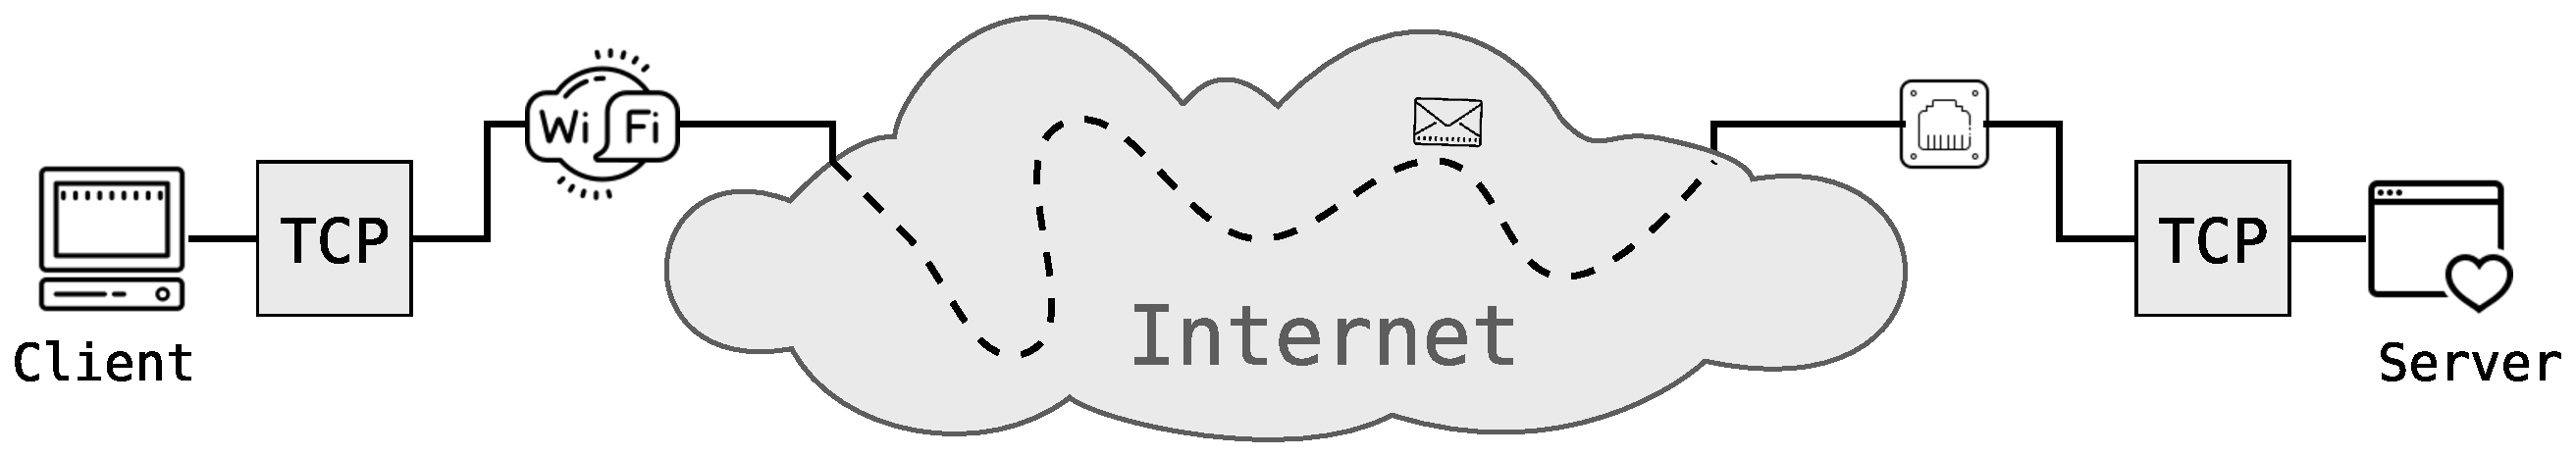
\includegraphics[scale=0.28]{../illustrations/introduction/TCPConnection.pdf}  
		\caption[Caption for the list of figures.]{Simplified illustration of TCP where the data exchange happens along a single fixed connection. The choice of the path taken cannot be influenced by the endpoints, in the illustration indicated by the dashed line.}
		\label{fig:IntroTCP}
	\end{center}
\end{figure}

\section{Multipath TCP (MPTCP)}

MPTCP stands for Multipath TCP and is an extension to TCP. It works exactly like TCP, with the only difference that all available network interfaces of a computer are used for the connection. This means that when the user visits his favorite website, MPTCP creates not just one connection, but one sub-connection, a so-called flow, for each interface available. Nowadays devices often have multiple attachment points to the Internet. So MPTCP creates, as illustrated in Figure \ref{fig:IntroMPTCP}, one flow via WLAN, one via cable and maybe even one via an analog dial-up modem. Thanks to these multiple flows, the protocol can improve reliability and performance. However, also with MPTCP, endpoints cannot influence what paths are taken by the individual flows. 

\begin{figure}[H]
	\begin{center}
		\def\svgwidth{1\textwidth}
		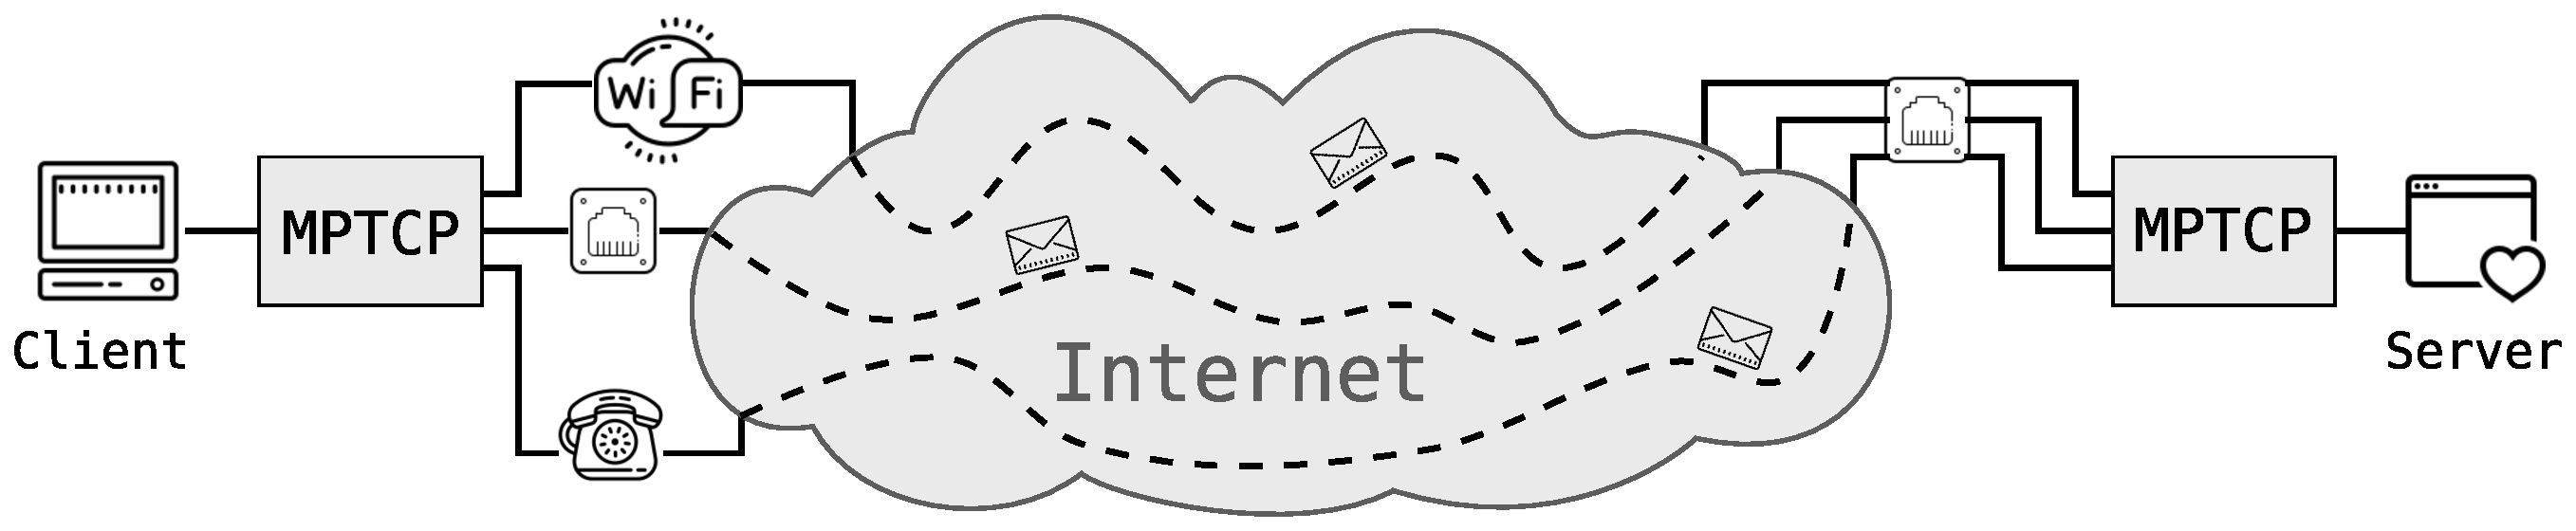
\includegraphics[scale=0.28]{../illustrations/introduction/MPTCPConnection.pdf}    
		\caption[Caption for the list of figures.]{Simplified illustration of MPTCP, where the endpoints use all available network interfaces for the data exchange. As for TCP, the choice for the paths taken cannot be influenced by the user.}
		\label{fig:IntroMPTCP}
	\end{center}
\end{figure}

\section{SCION}

Scalability, Control and Isolation on next-generation Networks or SCION for short is a new type of internet architecture, which has been developed by ETH Zurich for several years. SCION re-implements existing Internet protocols taking known vulnerabilities into account. It is more resource-efficient and reduces the supremacy of individual actors through its decentralized infrastructure. An important feature of the architecture, illustrated in Figure \ref{fig:IntroSCION}, is that endpoints can determine the path taken by its data through the network. Senders can choose the path along which they want to send their data, receivers can choose from which paths they want to receive data.

\begin{figure}[H]
	\begin{center}
		\def\svgwidth{1\textwidth}
		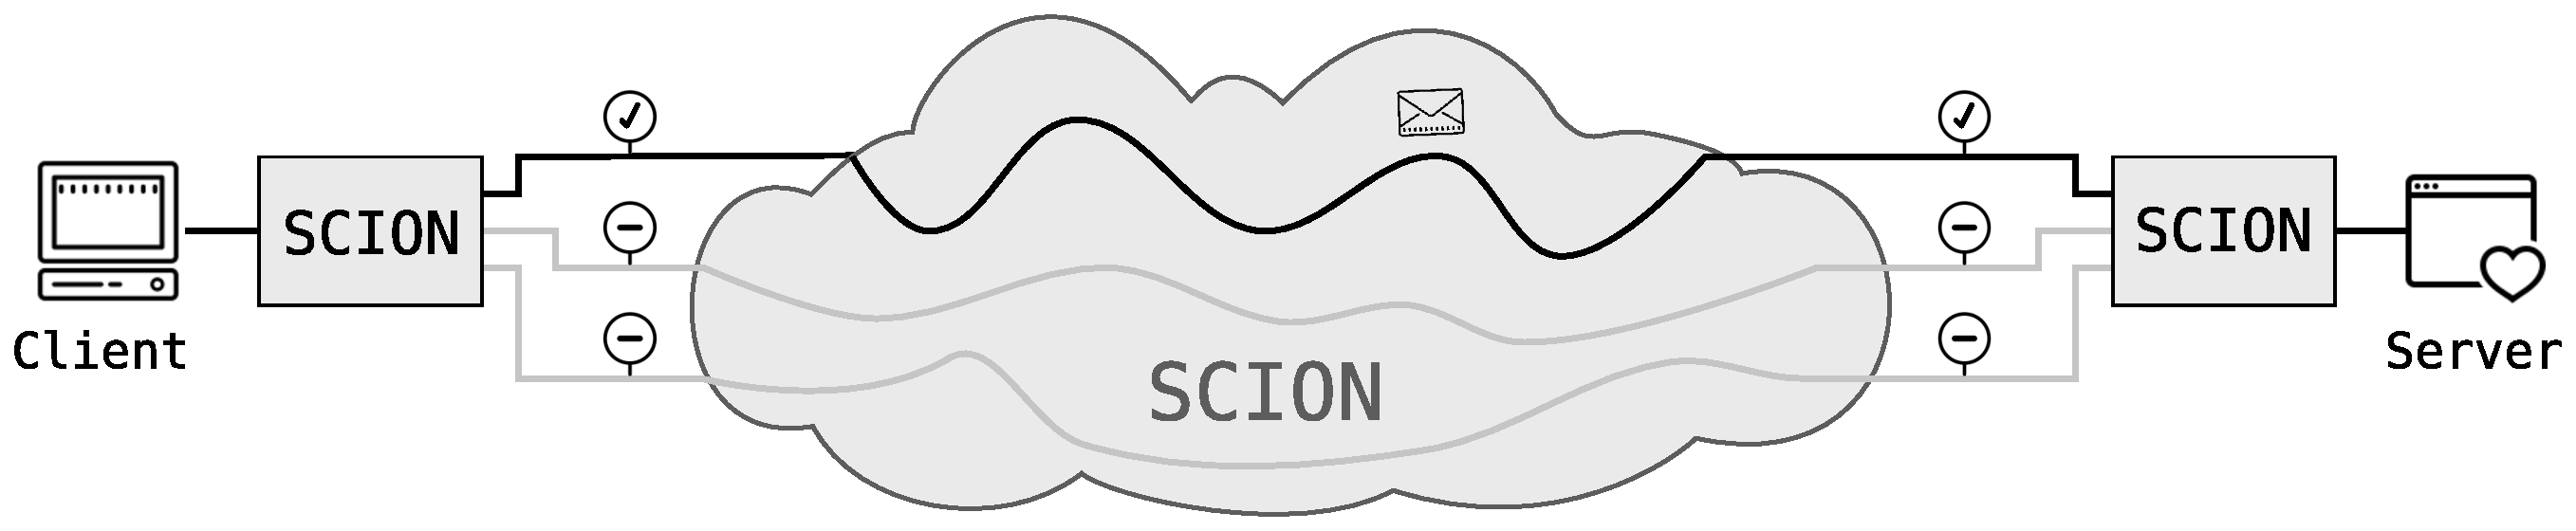
\includegraphics[scale=0.28]{../illustrations/introduction/SCION.pdf}
		\caption[Caption for the list of figures.]{Simplified illustration of the SCION internet architecture where the endpoints can determine which paths their data takes through the network.}
		\label{fig:IntroSCION}
	\end{center}
\end{figure}

\section{Shila}

\subsection*{Functionality}

Shila is the abbreviation for Shim Layer and is the main contribution of this work. It acts as a mediating layer and enables the use of MPTCP in the SCION internet architecture; illustrated in Figure \ref{fig:IntroRoleOfShila}. 

\begin{figure}[H]
	\begin{center}
		\def\svgwidth{1\textwidth}
		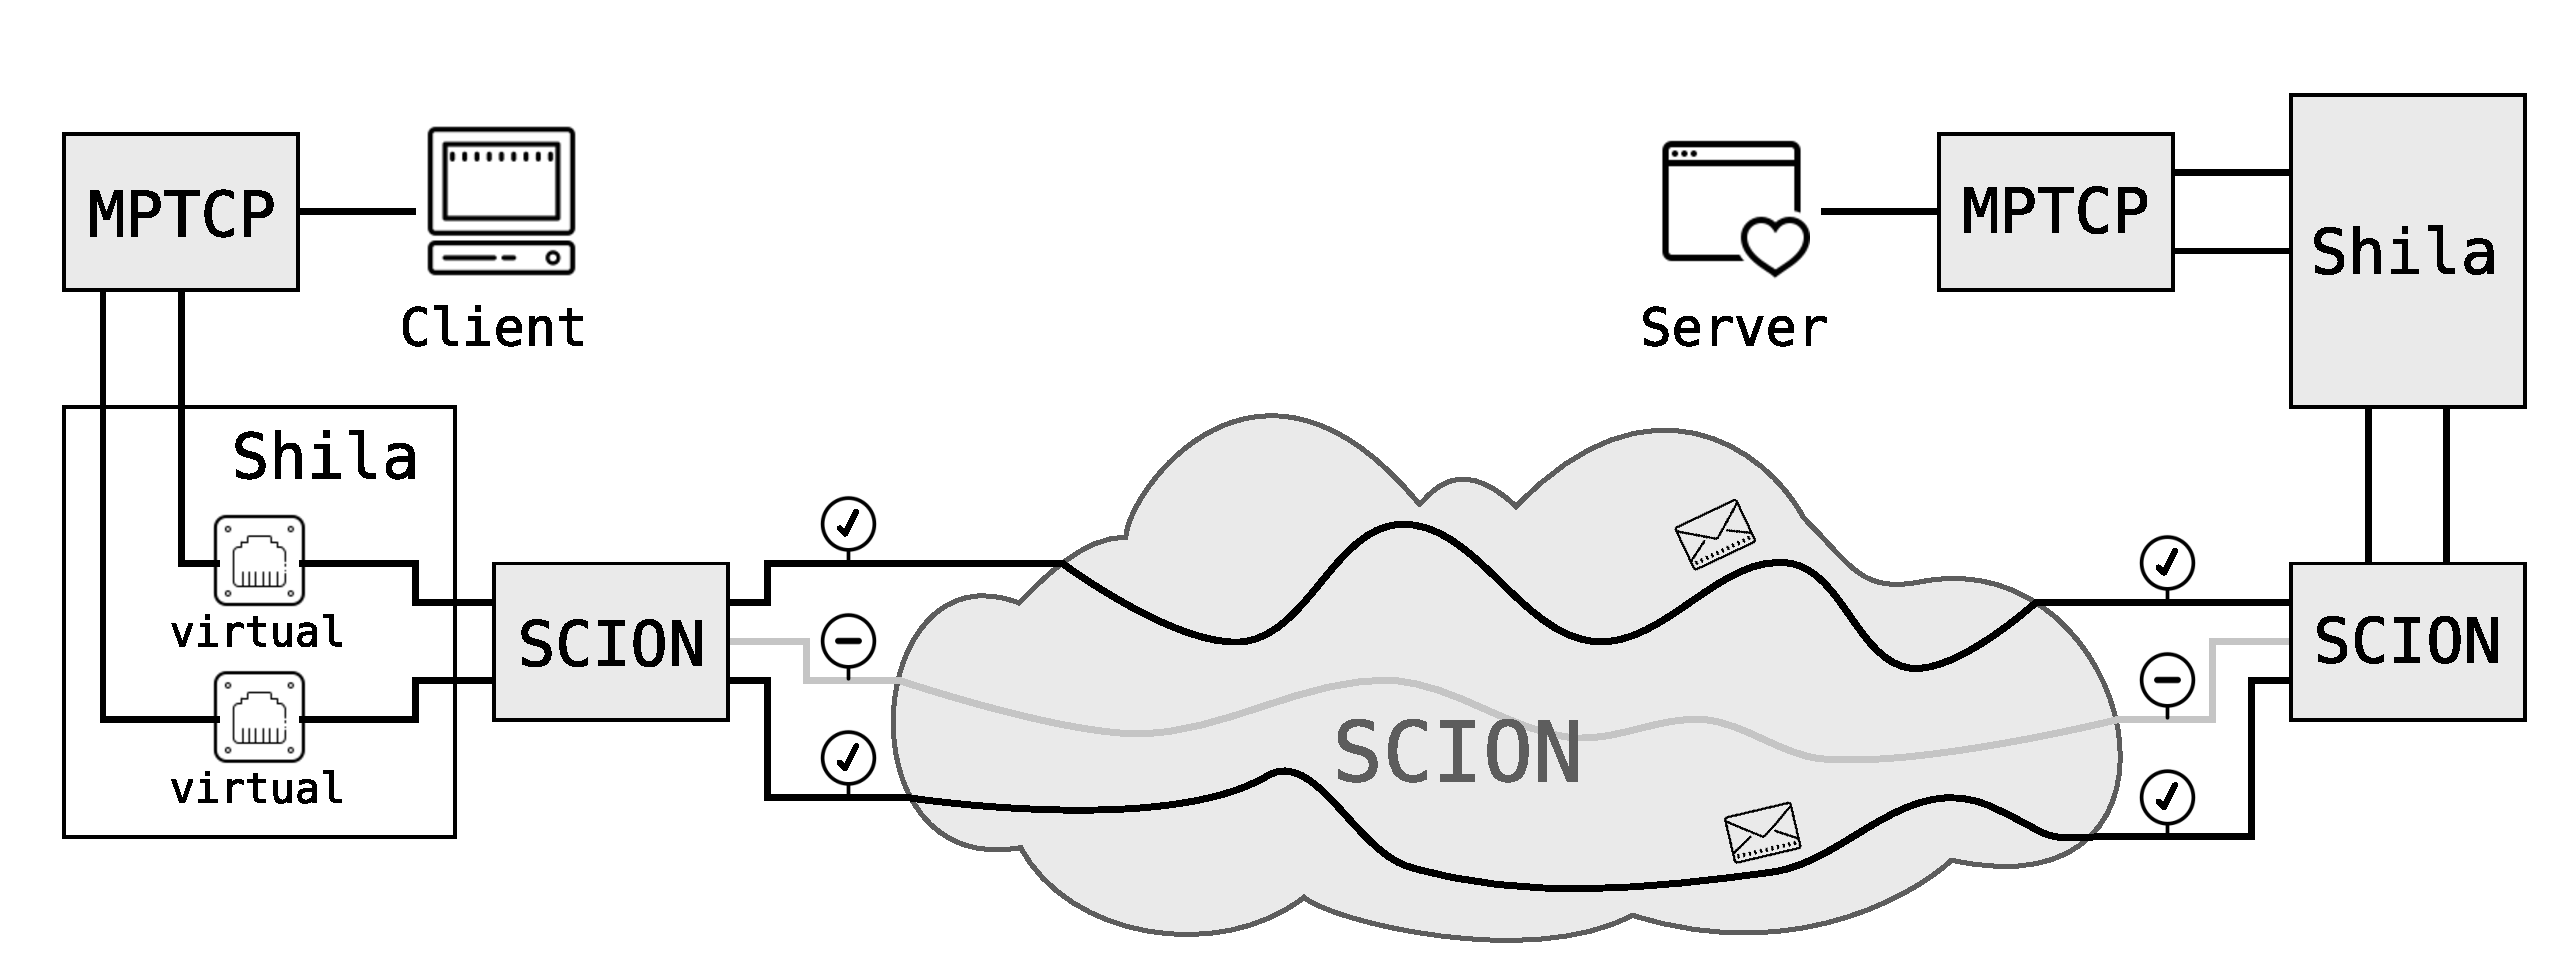
\includegraphics[scale=0.28]{../illustrations/introduction/Shila.pdf} 
		\caption[Caption for the list of figures.]{Simplified illustration of the functionality of Shila: It acts as an intermediate layer between MPTCP and SCION, provides virtual interfaces to MPTCP and redirects the intercepted flows through the SCION network.}
		\label{fig:IntroRoleOfShila}
	\end{center}
\end{figure}

Upon startup, Shila creates and monitors a user-selectable number of virtual network interfaces. A virtual interface is a fake connection to a network, which is perceived by the computer as a real one. If now someone visits his favorite homepage, Multipath TCP tries to connect to the server via these virtual interfaces. Shila detects this connection establishment and redirects the data flow.  For every flow created by MPTCP, the Shila instance creates a connection over SCION to the Shila instance running on the server and forwards the respective data traffic. The shim layer on the server side receives the data and distributes it through the MPTCP functionality to the server application.

\subsection*{Benefit}

The new internet architecture SCION offers great advantages over the existing Internet in terms of security and reliability. However, the transfer from such an established infrastructure as the current Internet to new technology is a big challenge. Applications rely on established programming interfaces and protocols and are programmed accordingly. A re-implementation of all software so that it can be used in a new architecture seems utopian. For the deployment of SCION, it is therefore of great importance that existing applications can be used in the new network with as little effort as possible. The implementation of Shila enables exactly this. All applications that use TCP for their communications can be operated via SCION without the need for internal changes. With Shila, your favorite TCP application can be run over SCION without much effort - a good reason to try the new infrastructure.

If the endpoints furthermore support MPTCP, the application can additionally benefit from the advantages of the multipath protocol and the support of multiple paths in SCION. But not only that, with Shila in its mediating role in between, there is further potential. To give a possible example, let's look at the use of MPTCP in today's Internet. It is quite possible that several flows of an MPTCP connection use the same link for certain parts of the path on the Internet. In order not to disadvantage other users, a fairness algorithm\footnote{Ensuring fairness is part of Congestion Control. However, to keep the introduction as generally understandable as possible, we don't use this term here.} monitors and controls the use of bandwidth. This is to ensure that all flows of an MPTCP connection going through the same link do not have more bandwidth available than the connection of another user. As we have seen, the endpoints on the Internet today are unaware of the paths their data takes. The same applies to the fairness algorithm, it has also no idea what paths are taken and can therefore not tell whether shared sub-paths exist or not. It has to act conservatively. If we use Shila to run our applications with MPTCP over the SCION network, Shila could ensure that no links are shared when choosing the paths of the individual flows. This makes it possible to disable the fairness algorithm or at least make it less strict, which results in better performance of the data transfer.
\chapter{Related Work}
\label{chap:RelatedWork}

In this chapter, we provide the reader with points of reference for related work and technologies. %As far as we know there is no work directly comparable to this one.

A detailed review of the development of multipath transport protocols gives the survey \cite{MultiPathSurvey}. It discusses reasons for the paradigm shift from single to multipath and the challenges of this transition. Furthermore the Stream Control Transmission Protocol (SCTP) \cite{SCTPWiki, rfc4960} and Multipath TCP (MPTCP) \cite{Barre2011, Raiciu2012, MPTCPWebMain,rfc6824}, the two most famous protocols in these area, are investigated.

SCTP shares several characteristics with TCP \cite{rfc793}. Both protocols are reliable, connection-oriented and use a rate-based mechanism for Congestion Control. Unlike with TCP, with SCTP a connection can consist of multiple streams, either used in a multiplexed fashion or simultaneously. This prevents the protocol from suffering from the Head-of-line blocking problem \cite{HOLBlocking} which is an issue with TCP. SCTP furthermore supports multihoming, a feature originally only intended to be used for failover. However, works like Concurrent multipath transfer SCTP (CMT-SCTP) \cite{1709949} or wireless multipath transfer SCTP (WiMP-SCTP) \cite{8205908} propose efforts to benefit from the availability of multiple paths by using them concurrently. The Stream Control Transmission Protocol appeared when TCP had already established itself. Making a change to SCPT would require adjustments to the applications and network stack, the most important factors why the protocol was not successful \cite{WhyNotSCTP}.

Multipath TCP (MPTCP), as an extension to TCP, is the most recognized approach to multipathing. It can be used by all TCP applications without any changes to their implementation. With MPTCP, multiple paths are used for the data exchange within a single connection. This functionality for example provides advantages in the field of smartphone use. The protocol facilitates the combination of WLAN and cellular access \cite{MPTCPStudyWirelessAndCellular} or allows fluid handovers between individual connection points \cite{MPTCPStudyHandover}. Well-known smartphone vendors such as Apple, LG or Samsung rely on Multipath TCP in their devices for the pleasant switch between 4G and Wi-Fi \cite{MPTCPInSmartphones}. In addition to mobile phones, for example also data centers benefit from better performance thanks to MPTCP \cite{RBPGWH11}.

In \cite{MPQUICPaper}, the implementation of an extension for QUIC \cite{quic-transport-29, QUICChromium}, called Multipath QUIC (MPQUIC), is presented. QUIC itself is a relatively recently developed protocol running on top of UDP. Similar to SCTP, QUIC supports several streams but not the use of more than one path. MPQUIC enables the protocol to use multiple paths. An in-depth discussion of (MP)QUIC and an investigation of MPTCP with the focus on use cases with smartphones, devices predestined for multi-homing, is given in \cite{MPQUICThesis}.

Increased demands on reliability and performance as well as the availability of multiple network interfaces have led to the development of the mentioned multipath protocols.  Although the Internet was not originally designed for the use of multiple paths, it allows it.  This is contrary to new internet architectures such as NEBULA \cite{NEBULA} or SCION \cite{SCIONPaper, SCIONBook}, where multipathing is an inherent part of the design and a cornerstone of security and reliability. 

The TUN/TAB drivers \cite{TUNTAPDriver} provide accessibility of virtual network devices to applications in userland. This functionality is mainly used for tunneling, for example by VTun \cite{VTun} or OpenVPN \cite{OpenVPN}.


\chapter{Important Concepts}
\label{chap:Concepts}
In this chapter, we present the most important building blocks on which this work is based. It is meant to refresh the reader's understanding should allow to consume this thesis in a self-containing manner and to place the work in a larger context. The three building blocks are the Transmission Control Protocol (TCP), Multipath TCP (MPTCP) based on it and finally the new internet architecture SCION. These three concepts are summarized in the corresponding order in the following sections.

\section{Transmission Control Protocol (TCP)}
\label{sec:TCP}

This recap about the widely used transport protocol TCP is mainly inspired by the worth reading summary \cite{TCPSummary}.

The Transmission Control Protocol (TCP) is one of the main protocols in today's Internet. Its two main developers, Vint Cerf and Bob Kahn, started working on the protocol in 1974. The original specification was written in 1981; defined in the RFC document number 793 \cite{rfc793}.

TCP is a byte stream, connection-oriented and reliable transport protocol. In the OSI model, it is situated between the application layer above and the network layer below. TCP receives the data in a byte stream from the application. It is up to the protocol to partition this stream into so-called TCP segments in order to transmit the data in manageable pieces to the receiver. Before two endpoints can exchange data over TCP they must first agree upon the willingness to communicate; hence connection-oriented. Similar to a call with a telephone, first a connection has to be established before the two parties can exchange information. We describe the procedure of a TCP connection establishment and termination later in this section. To ensure reliable data transfer TCP uses different mechanisms. A per-segment checksum enables the receiver to detect crudities in the transferred data, furthermore is everything, that is received multiple times, discarded by the receiving side. It is also the receiver that ensures that the received data is transferred to the application in the correct order. TCP also has a retransmission functionality that ensures delivery of the data in the case of data corruption or loss. The successful reception of data is confirmed by the receiver with a positive acknowledgment. If the sender does not receive such positive acknowledgments for a certain period of time, it will resend the data. 

\subsection*{TCP Segment}

TCP partitions the byte stream into TCP segments consisting of a header and a data part. Figure \ref{fig:TCPSegment} depicts a valid format of a TCP segment with its different fields. In the following, the fields most important for the understanding of the TCP are described in more detail. 

\begin{figure} [H]
	\begin{center}
		\def\svgwidth{1\textwidth}
		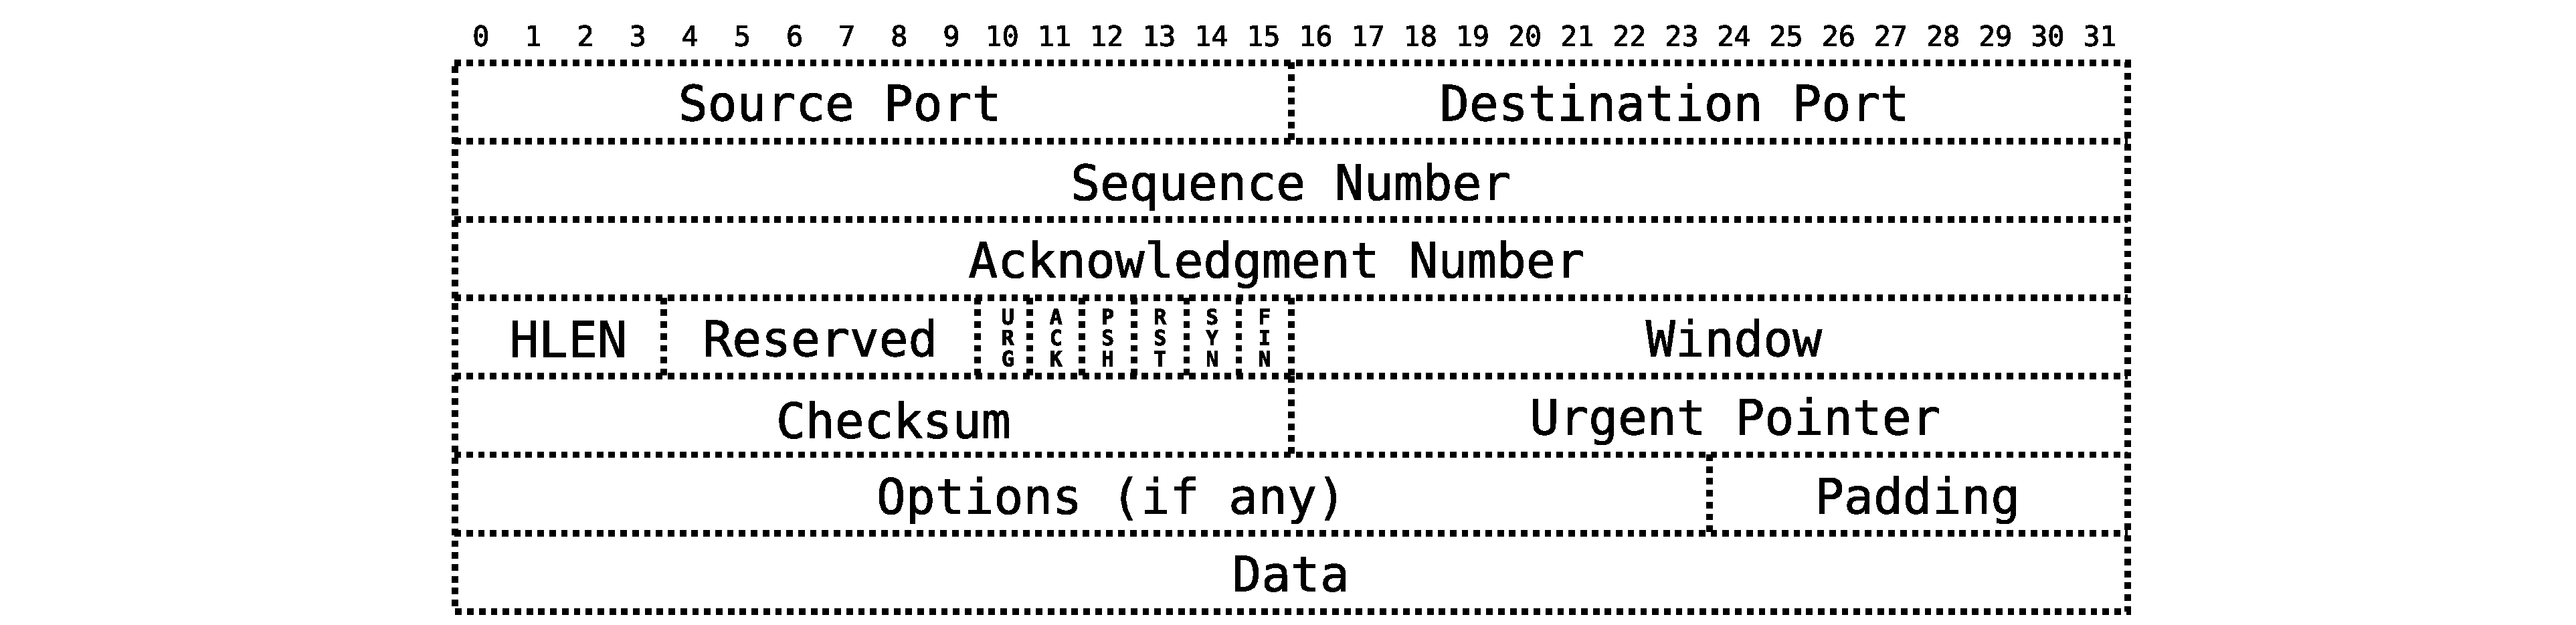
\includegraphics[scale=0.2]{../illustrations/importantConcepts/TCPSegment.pdf}  
		\caption[]{Illustration of a TCP segment.}
		\label{fig:TCPSegment}
	\end{center}
\end{figure}

{\small \textbf{Source Port:} 16-bit number tagging the application the segment originated from within a sending endpoint. \smallskip\\
\textbf{Destination Port:} 16-bit number tagging the application the segment is destined for on a receiving endpoint. \smallskip\\
\textbf{sequence number:} 32-bit number identifying the current position of the first data byte in the segment within the entire byte stream for the TCP connection. \smallskip\\
\textbf{Acknowledgment Number:} 32-bit number telling the receiver which data byte the sender is expecting next. It is always one greater than the most recently received data byte and only valid if the ACK control bit is set. \smallskip\\
\textbf{ACK (Control Bit):} If set, then the acknowledgment number is valid. \smallskip\\
\textbf{Window:} 16-bit number used by TCP for flow control. It specifies the number of bytes the sender of this segment is currently willing to receive. \smallskip\\
\textbf{SYN (Control Bit):} Sender and receiver use this bit during the connection establishment to synchronize their sequence numbers.  \smallskip\\
\textbf{FIN (Control Bit):} This bit is part of the connection termination. It is set by the sender if its byte stream has reached the end. \smallskip\\
\textbf{Options:} Provides space for additional optional parameters that one may want to exchange between sender and receiver. 
}
 
Note that a single TCP connection is globally uniquely identified by a complete pair of IP addresses (source and destination) together with a complete pair of TCP ports (source and destination).

\subsection*{Connection Establishment, Data Transfer and Termination}

TCP is connection-oriented, meaning that there is a virtual connection between two endpoints exchanging data. Such a virtual connection runs through three stages: connection establishment, data transfer and connection termination.

\paragraph{Connection Establishment}

Two hosts, A and B, willing to communicate establish a connection by exchanging a predefined set of messages known as the Three-Way Handshake. Figure \ref{fig:TCPConnectionEstablishmentAndTermination} on the left side illustrates this sequence. 

\begin{figure}[H]
	\begin{center} 
		\def\svgwidth{1\textwidth}
		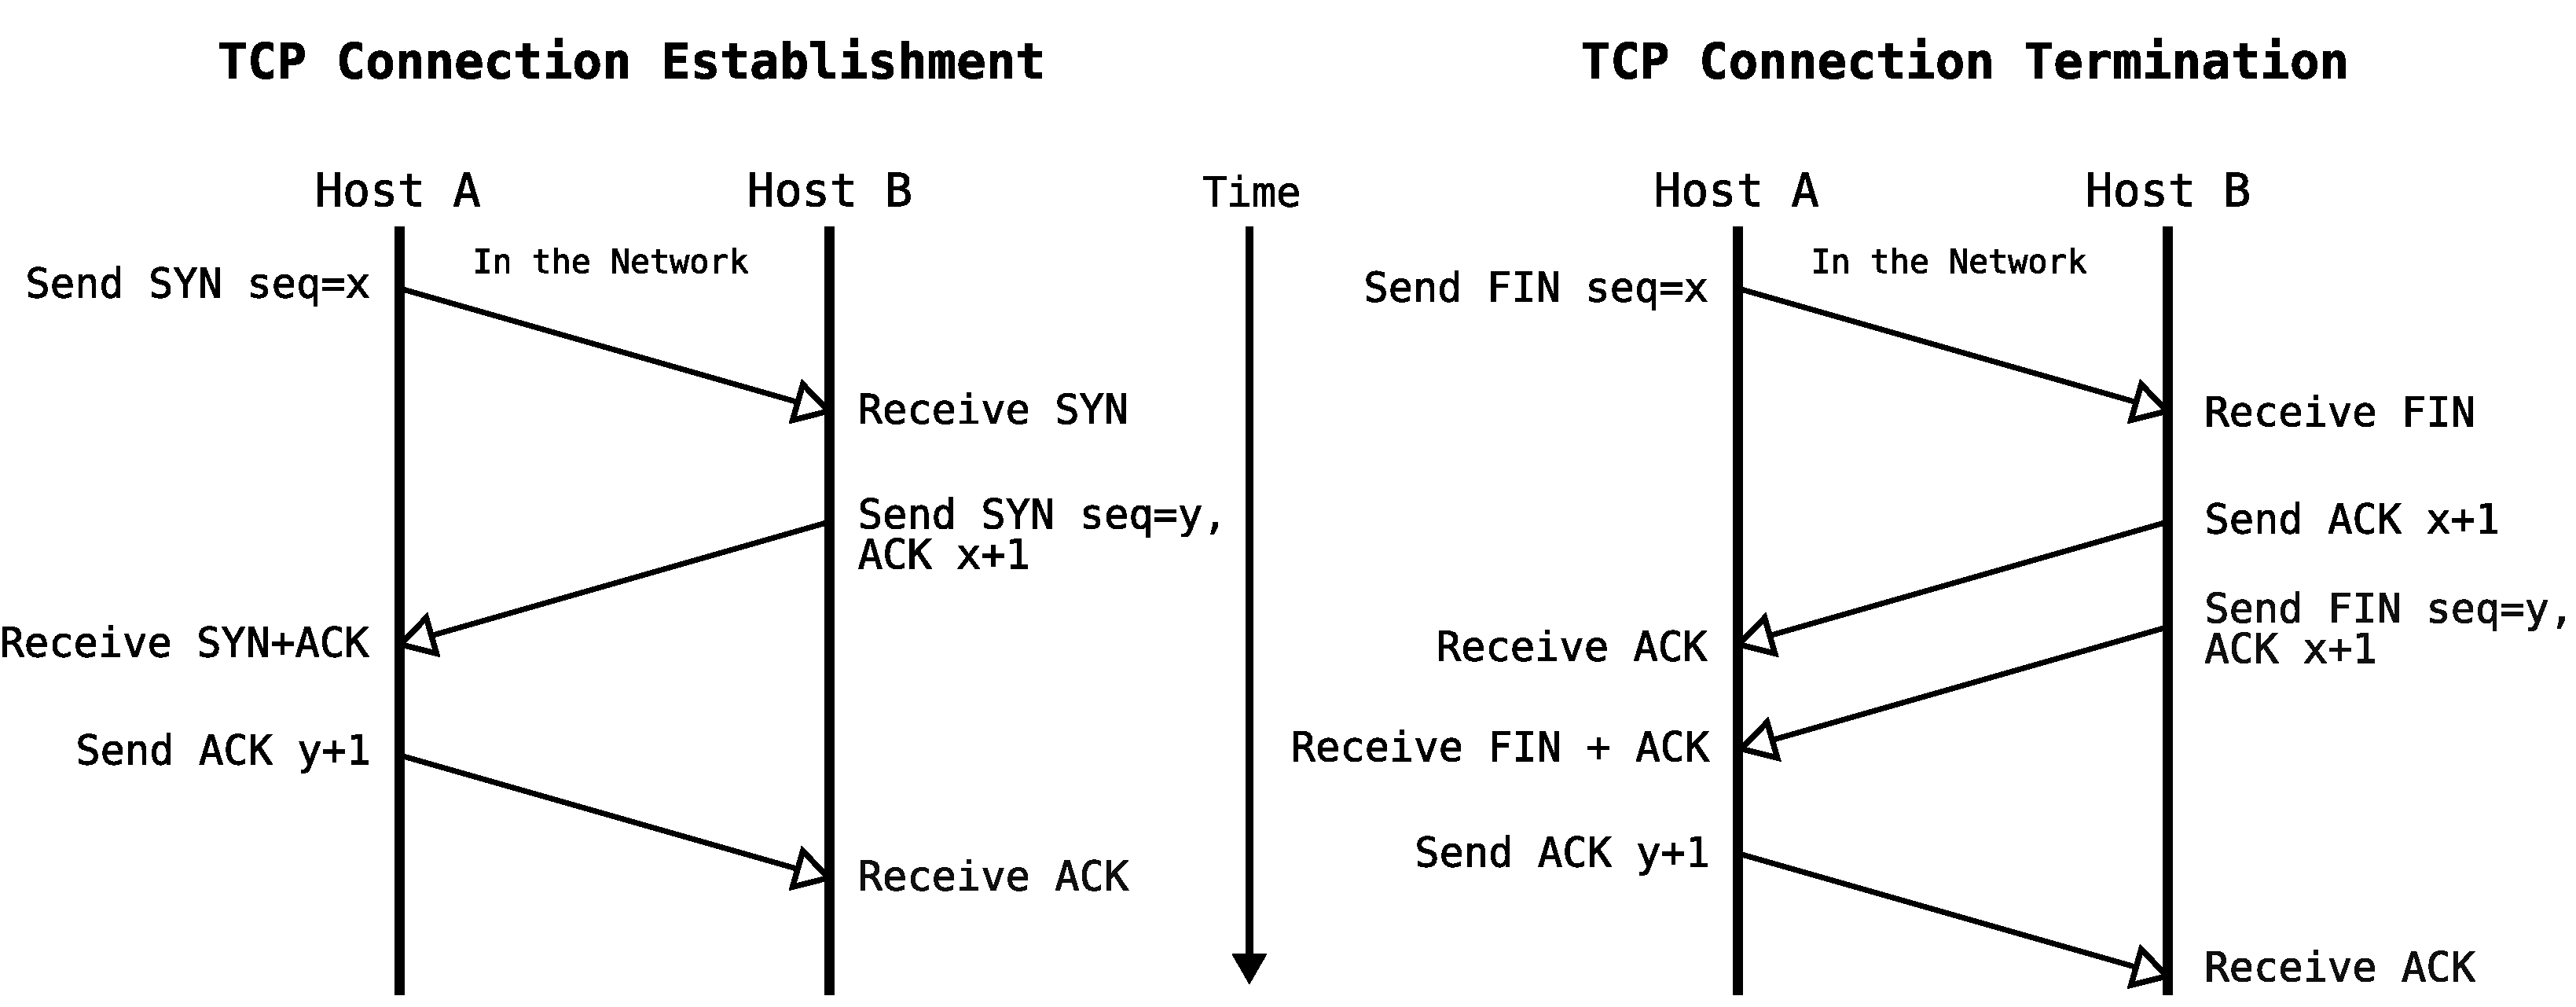
\includegraphics[scale=0.24]{../illustrations/importantConcepts/TCPHandshake.pdf} 
		\caption[]{Illustration of the TCP connection establishment (l.) and TCP connection termination (r.) messages exchange.}
		\label{fig:TCPConnectionEstablishmentAndTermination}
	\end{center}
\end{figure}

Host A as an initiator of the connection sends a segment containing an initial sequence number x and the SYN control bit set to Host B. \smallskip\\Host B processes the received segment and answers with a segment of its own. It contains an initial sequence number y and has the SYN control bit set. Furthermore assigns Host B x+1 to the acknowledgment number and sets the ACK control bit. This indicates that the next byte expecting from Host B should contain data starting with sequence number x+1. \smallskip\\ Host A finishes the connection establishment phase upon reception of Host B's SYN+ACK. It sends a last acknowledgment to Host B, indicating that the next expected byte should start with sequence number y+1.

\paragraph{Data Transfer}

Once the Three-Way Handshake is completed, the two hosts can exchange data with each other. Important functionalities of the data transfer are flow control and congestion control. We discuss these concepts later, for now, we just focus on some key ideas. 

In a basic TCP implementation, segments are put into the network by the sender as long as there is data available and as long as the window announced by the receiver is not exceeded. The receiver consumes the segments and acknowledges them by sending back positive acknowledgments together with its current position in the byte stream. The announcement of the current window size is also included in these messages sent back. If data gets lost or duplicated, a hole may exist in the byte stream. The receiver continues to acknowledge the most current contiguous position in the byte stream accepted so far.

The sender must halt transmission in the case where data ready to be sent will exceed the receivers advertised window size. Upon reception of further positive acknowledgments announcing a window size greater than zero, the sender can continue delivering the data.

If there is no data to send, TCP waits patiently until either there is some again or the other end of the connection sends data to receive.  

\paragraph{Connection Termination}

A TCP connection is completely terminated by the exchange of four segments as depicted on the right side of Figure \ref{fig:TCPConnectionEstablishmentAndTermination}. Since the protocol is full-duplex, both ends must be torn down independently. To initiate this process the FIN control bits are used. 

As soon as the application running on Host A wants to close the connection, a FIN segment is sent from Host A to Host B. Upon reception of this segment Host B acknowledges it and notifies its destination application about the termination request. As soon as this application shuts down the connection as well, Host B sends out a FIN segment which is finally acknowledged by Host A.

\subsection*{Flow Control}

Flow control is an important part of the data transfer in TCP. Its purpose is to properly match the transmission rate of the sender to that of the receiver and the network. For performance reasons, one is interested in a transmission rate that is high enough without overwhelming the receiver or the network. TCP uses the window field to adjust the rate of flow between TCP endpoints. This concept is called sliding window. In every segment, the receiver specifies with the window field how much data it is willing to buffer. The sender can only send up to that amount of data before it has to wait for further acknowledgments and window updates from the receiver. 

\subsection*{Congestion Control}

Another major part of the data transfer in TCP is congestion control. However, this term is misleading, since it rather should be called congestion avoidance. TCP itself cannot control the congestion, it rather tries to avoid congestion using different mechanisms, which are briefly discussed in the following. 

\paragraph{Slow Start}

Slow start is a mechanism used by the sender to control the sending rate. Hereby, the rate of acknowledgments returned by the receiver controls the rate at which the sender can transmit data. At the very beginning of a TCP connection, the congestion window is initialized to one. With every positive acknowledgment received, the congestion window is increased by one. The sender can send the minimum of this congestion window and the advertised window of the receiver, denoted as transmission window. Unlike the name suggests, slow start is by no means slow. In a congestion-free network with good response time, the congestion window doubles for every round-trip-time. The increase of the congestion window will continue until the maximum transmission window is reached or until congestion finally occurs.

\paragraph{Congestion Avoidance}

The congestion avoidance algorithm has two mechanisms to detect network congestion. If the blockage is indicated through the reception of duplicate acknowledgments, the transmission window is halved and the fast retransmit and fast recovery mechanism take over. If the congestion was indicated through a timeout of the retransmission timer, then the sender is put back into slow start mode, i.e. the transmission window is set to one. After running into congestion, the congestion window is again increased using slow start. However, it is only used up to the halfway point where congestion originally occurred. After reaching this point, the congestion window is just increased by one for all segments in the transmission window that are acknowledged. The linear growth from this point onward makes sure that TCP increases its transmission rate more slowly towards the previous congestion point.  

\paragraph{Fast Retransmit}

If the sender receives an acknowledgment multiple times, it is not clear if it is because a segment was lost or simply that a segment was delayed and received out of order at the receiver. If the latter is the case, it should not take too long until the latest expected acknowledgment arrives. Typically, for simple out of order condition, not more than one or two duplicated acknowledgments should be received. More duplicates are a strong indication that a segment was lost. Upon reception of three duplicated acknowledgments, the sender does not wait until the retransmission timer expires but resends the segment immediately and enters Fast Recovery.

\paragraph{Fast Recovery}

Duplicate acknowledgments can only be generated when a segment is received at the receiver. That is, as long as the sender receives acknowledgments it knows that there is data flow through the network. The loss of a segment was probably just a rare event, instead of reducing the flow drastically by using slow start again the sender just enters congestion avoidance without decreasing the size of the congestion window too much. This behavior allows for higher throughput in cases of only moderate congestion.

\subsection*{Conclusion}

TCP is a rather complex protocol that handles an enormous amount of functionality in today's Internet. The presented discussion gives only a small insight into the scope of TCP. However, it should provide the reader with the necessary understanding so that the extension to TCP, namely Multipath TCP, discussed in the next section is more easily accessible.

\section{Multipath TCP (MPTCP)}
\label{sec:MPTCP}

In this section, we introduce Multipath TCP. The presented summary is based on \cite{Barre2011, Raiciu2012, Wischik2011} and the RFC document number 6824 \cite{rfc6824}.

\subsection*{Basics}

In times where most hosts are equipped with multiple physical interfaces, a protocol that binds each connection to a single interface does not exhaust the potential of the infrastructure. TCP is not capable of using the multiple paths to the Internet available for an increase in connection redundancy and performance. Multipath TCP, as an evolution of TCP, is an attempt to utilize the multiple paths available to gain robustness and performance advantages.

Multipath TCP allows an unmodified application to start what it believes a regular TCP connection using the well-known API for TCP. If both endpoints support the use of MPTCP, multiple flows are established under the hood. The data is shared among these flows, where most data is sent out on the least congested path. If the use of MPTCP is not supported a regular TCP connection is established instead. Multipath TCP works in all scenarios where TCP currently works. By using an appropriate congestion control MPTCP furthermore ensures that other, regular TCP connections present in the network are not disadvantaged. 

\subsection*{Connection Setup}

MPTCP uses the TCP Three-Way Handshake to set up the initial connection, i.e. the main-flow. The sender includes the MP\_CAPABLE option in the SYN, which is also included in the returning SYN+ACK when the server is ready to use MPTCP. The sender concludes the Multipath TCP connection setup by including the MP\_CAPABLE option in the third packet of the handshake as well. The connecting entities fall back fo regular TCP if not all segments being exchanged as part of the Three-Way Handshake contain the respective option. The MP\_CAPABLE option itself contains a 64-bit key generated by the sender and the receiver, later used to verify the authenticity of additional flows. The sequence of segments exchanged for an MPTCP connection establishment between two Host A and B is illustrated in Figure \ref{fig:MTCPConnectionEstablishment}.

\begin{figure}[H]
	\begin{center} 
		\def\svgwidth{1\textwidth}
		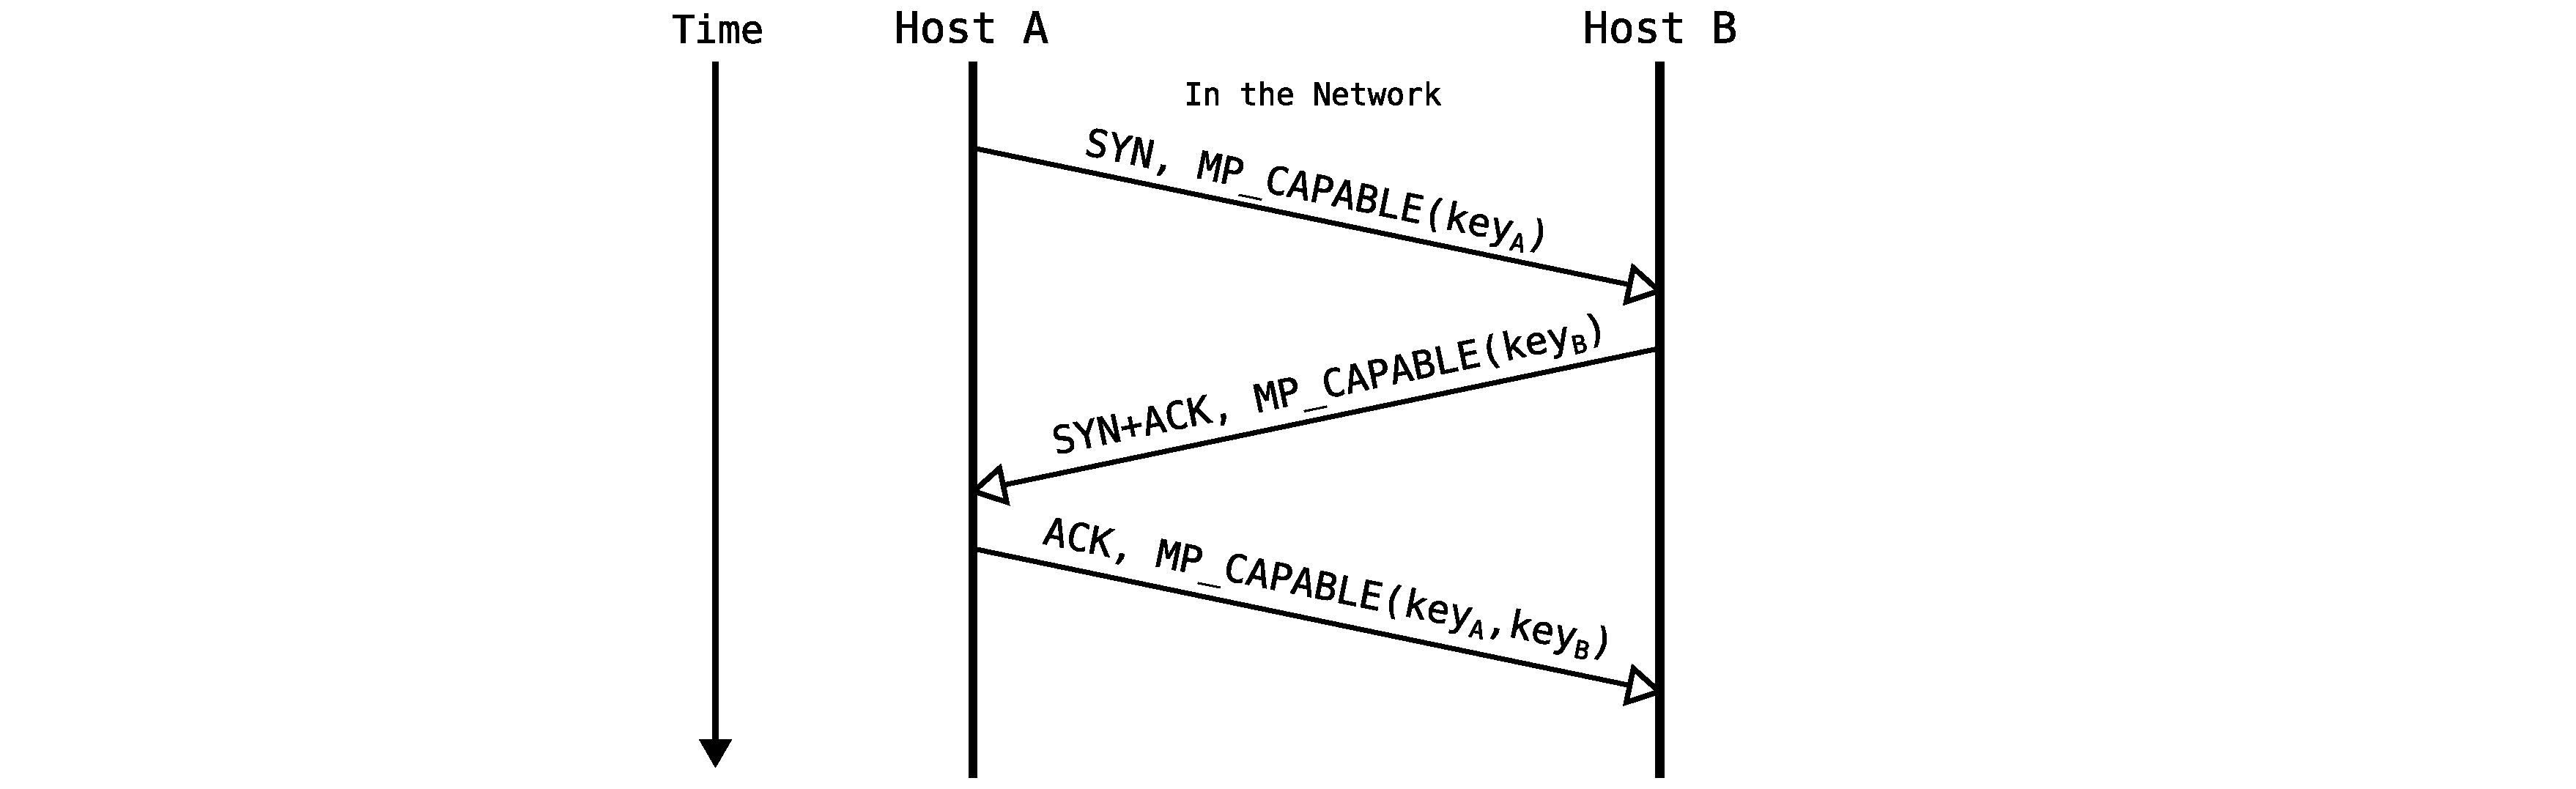
\includegraphics[scale=0.24]{../illustrations/importantConcepts/MPTCPHandshake.pdf} 
		\caption[]{Illustration of the sequence of segments exchanged for the MPTCP connection setup. The MP\_CAPABLE option has to be included in all messages exchanged for the establishment to succeed.}
		\label{fig:MTCPConnectionEstablishment}
	\end{center}
\end{figure}

\subsection*{Addition of Sub-flows}

Once a connection, i.e. the main-flow, has been established, further flows, so-called sub-flows, can be added. For this MPTCP again performs a regular TCP Three-Way Handshake using addresses or ports of additionally available interfaces. To add the sub-flow, the MP\_JOIN option has to be included in any segment part of the handshake. This option holds the message authentication code (MAC) of the keys exchanged in the previously described initial connection setup. This measure makes it difficult for malicious third parties to hijack an existing connection. Furthermore includes the option a connection identifier, derived as a hash from the receiver's key, used to match new sub-flows with an existing connections main-flow. 

\subsection*{Data Transfer}

Data exchanged between client and server can be sent over any flow part of a Multipath TCP connection. To remain a reliable protocol, MPTCP must retransmit data over a different flow if a certain flow fails. This is achieved by making use of two different principles discussed in the following and illustrated in Figure \ref{fig:MPTCPDataTransfer}.

\paragraph{Flow and Data Sequence Number}

In Multipath TCP every flow is equivalent to a regular TCP connection using its own 32-bit sequence number space. With this flow sequence number, the current position within the entire byte stream transferred over a certain flow is identified. Additionally, MPTCP maintains a 64-bit data sequence numbering space, which is used by the DSS\_MAP and the DSS\_ACK option. The DSS\_MAP contains a mapping between the flow sequence number and the data sequence number. It is used by the receiver for correctly ordering the byte stream, possibly received disordered over the different flows, for the application.

\paragraph{Two different Acknowledgment Levels}

The acknowledgment of received data happens on two different levels. The regular TCP acknowledgment Number is used to confirm the reception of data on a flow connection level. Standard retransmission mechanisms, as discussed earlier, are used to recover from a segment loss indicated through the reception of multiple acknowledgments confirming the same flow sequence number. With the additional DSS\_ACK returned by the receiver as part of the ACK's, cumulative acknowledgments at a data sequence level are available. These allow MPTCP to detect the failure of a flow and to initiate the retransmission of lost data over a different flow.

\begin{figure}
	\begin{center}
		\def\svgwidth{1\textwidth}
		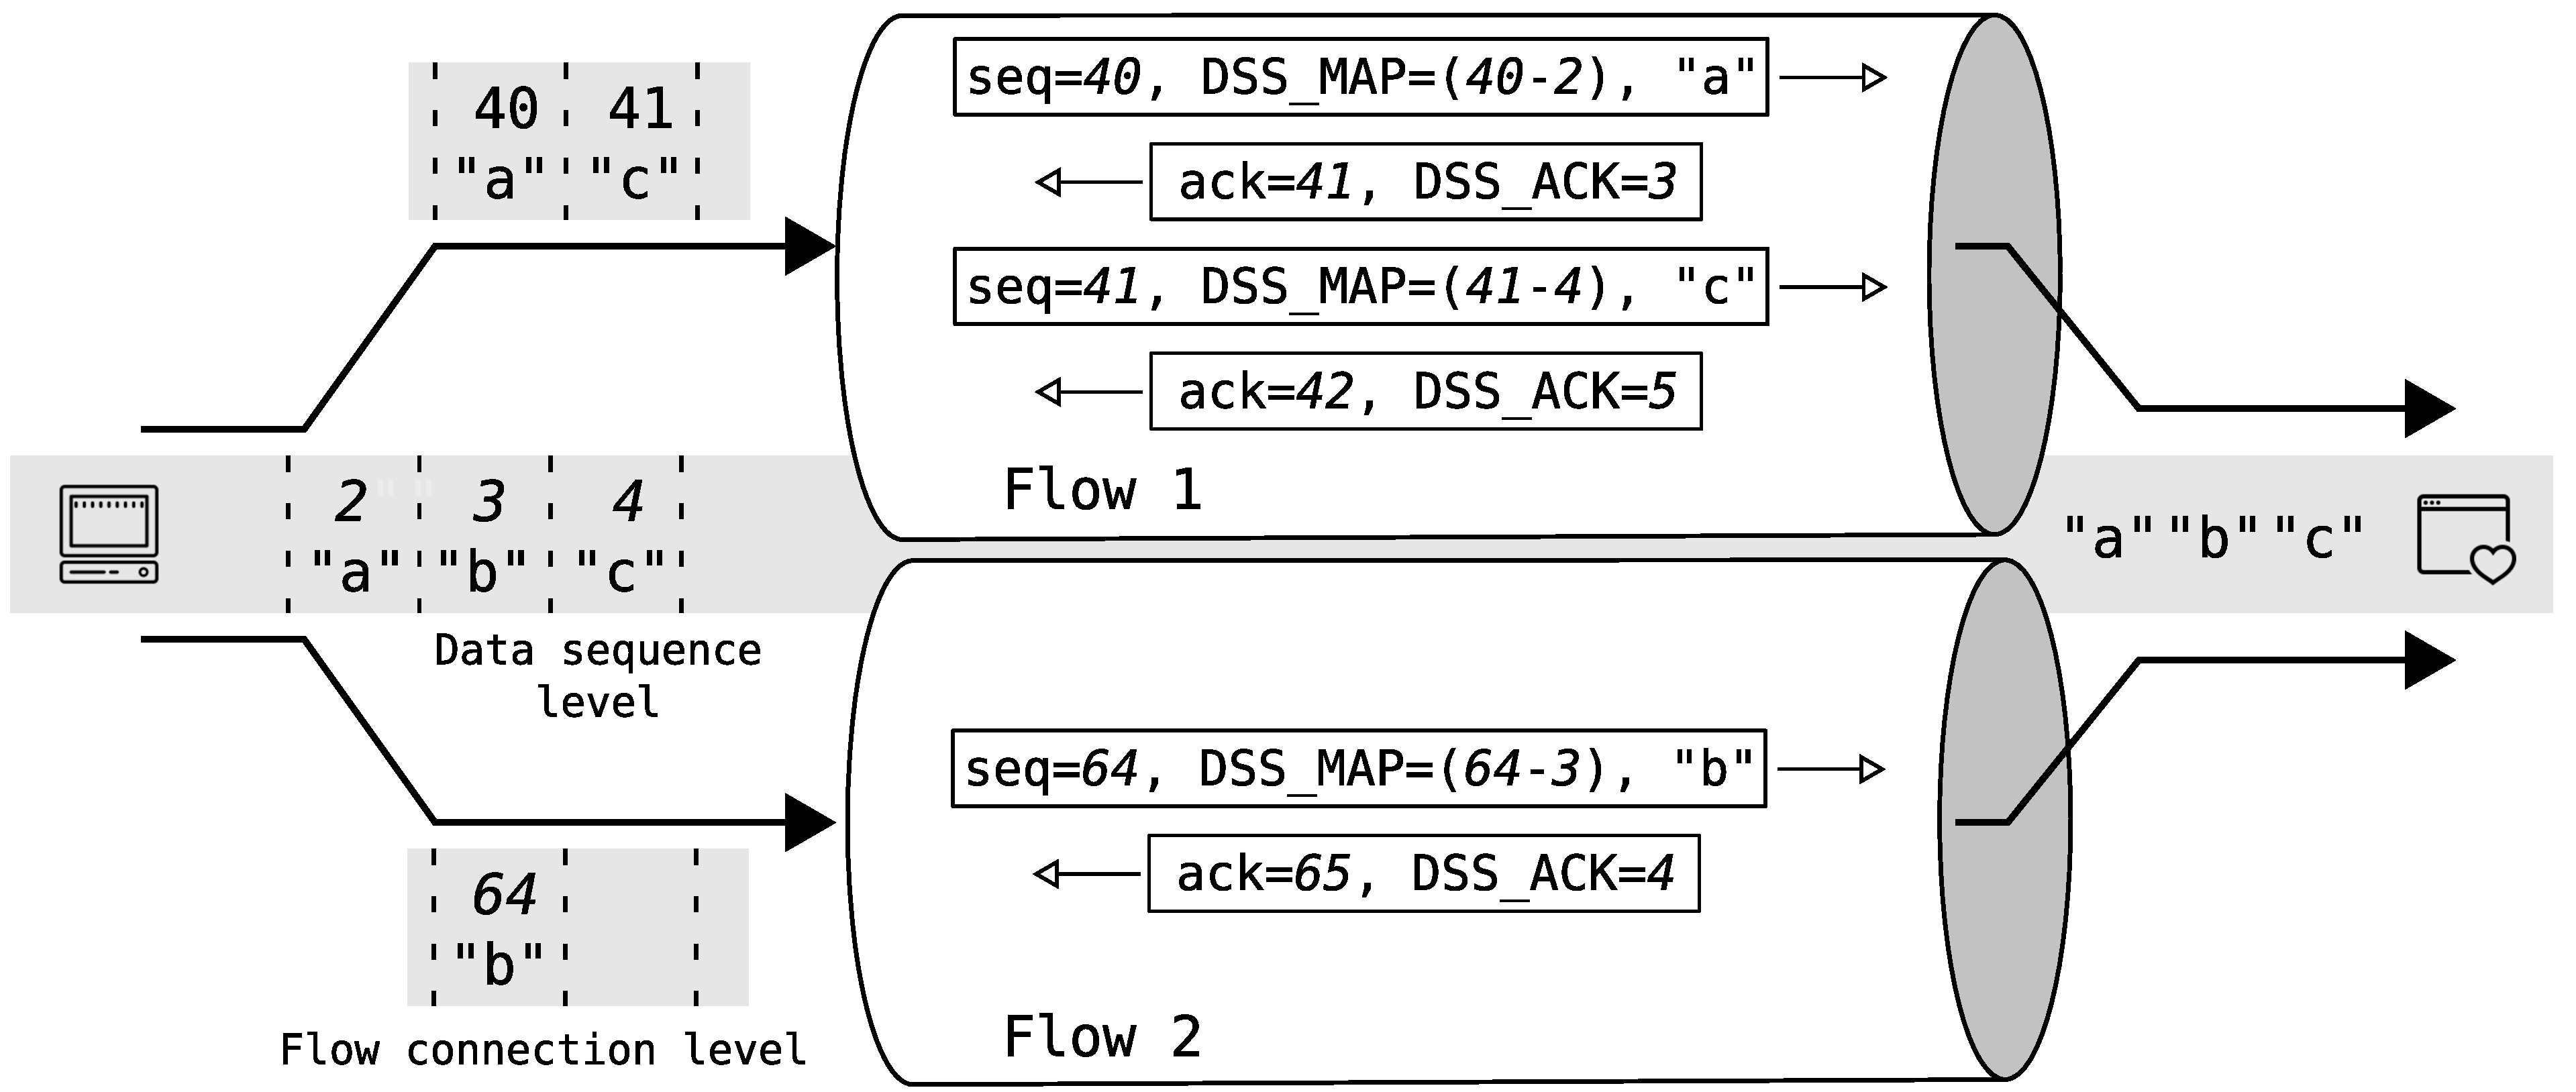
\includegraphics[scale=0.2]{../illustrations/importantConcepts/MPTCPDataTransfer.pdf}  
		\caption[]{Illustration of data transfer in MPTCP with two flows. The regular TCP sequence numbers are used to acknowledge data reception and trigger mechanisms for re-transmission on a flow connection level. With the additionally introduced DSS\_ACK's on a data sequence level, MPTCP is able to detect dying flows and can maintain the ordering of exchange data.}
		\label{fig:MPTCPDataTransfer}
	\end{center}
\end{figure}

\subsection*{Congestion Control}

One way to implement congestion control in MPTCP is to use conventional mechanisms on a flow connection level. This means that each TCP flow maintains its congestion window without affecting or being affected by other flows and their window. Possible congestion control could be any suitable for TCP, like the default AIMD approach \cite{rfc5681} mentioned in the previous section or derivatives like CUBIC \cite{rfc8312}. But with independent congestion windows for each flow, other users in the network are disadvantaged. Imagine that several flows of an MPTCP connection and a single external TCP connection share the same link. In this case, the MPTCP may use more bandwidth than it is entitled to.  This is possible because each flow is treated as a single, independent TCP connection. To eliminate this injustice MPTCP uses instead a congestion algorithm which makes the windows of the individual flows dependent on each other. One possible implementation hereby is the Linked Increase Algorithm (lia) \cite{rfc6356}, initially proposed by the community.  In the meantime, further developments, for example the Opportunistic Linked Increase Algorithm (olia) \cite{khalili-mptcp-congestion-control-05}  or the Balanced Linked Adaptation Congestion Control Algorithm (balia) \cite{walid-mptcp-congestion-control-04} are available.

\subsection*{Conclusion}

The benefits of MPTCP as an extension are promising, as already mentioned in Chapter \ref{chap:RelatedWork}, especially in the area of smartphone usage.  With this summary, we have by no means covered all facets of Multipath TCP. But it does provide a basis for understanding this work and how we try to benefit from the protocol as well. An overview of the current development around MPTCP can be found here \cite{MPTCPWebMain}.

\section{SCION}
\label{sec:SCION}

In the upcoming summary, we introduce the reader to the fundamental concepts of SCION. It is based on the SCION book \cite{SCIONBook} and a selection of videos \cite{SCIONWebVideos}. More information and the latest news about the development of SCION can be found on the official web site \cite{SCIONWebMain}.

\subsection*{Shortcomings of today's Internet}

We start by mentioning some of the Internet's shortcomings, more precisely the shortcomings of two important building blocks of it. Today's Internet is of great importance for the economy, politics and society worldwide. Despite this importance, the global infrastructure does not meet the requirements in terms of security and availability to any degree. The core of the Internet is based on a few protocols developed almost 30 years ago. The Internet Protocol (IP) and the Border Gateway Protocol (BGP) control most system-relevant functions, but have undergone only minimal development since their deployment and suffer from several shortcomings.

\paragraph{Internet Protocol (IP) and its Shortcomings}

IP handles the transport of packets between end-users along a single path through the Internet. It routes them from a starting point to a destination, the endpoints have no influence on or knowledge of the path the packets take. All units involved in the routing determine the next hop based only on the destination address and a routing table. For IP, one can note the following shortcomings: The protocol does not sufficiently separate the functionality of routing and forwarding, sudden updates of routing tables can adversely affect a path, e.g. change its direction or even break it. Furthermore, the protocol does not offer the end-user with the possibility to control or check the path his data takes through the Internet. This functionality would be desirable in many situations, e.g. allowing a sender to avoid sending its data through malicious nodes. Furthermore, the IP protocol is based on the use of routing tables. The high-performance lookup of next-hop destinations is energy-intensive and the routing tables can be maliciously exhausted.

\paragraph{Border Gateway Protocol (BGP) and its Shortcomings}

BGP is responsible for the exchange of routing information between independently operating autonomous systems, denoted as ASes, like Internet service providers (ISPs). These providers use BGP update messages to announce the IP prefixes which are reachable through their subnet. Each ISP can decide based on its criteria which announcements it wants to share further and which routes it wants to use. This traffic engineering is mainly driven by economically influenced policies. BGP also suffers from some shortcomings. It may take a considerable amount of time for the routing infrastructure to return to a stable state after new announcements have been made. Route changes directly affect forwarding and can lead to failures and interruptions of the data exchange. Furthermore, notifications affect all BGP entities that are present in the network. There is no hierarchy or isolation between individual areas. A single faulty BGP entity can severely disrupt the entire global routing infrastructure. Finally, BGP only allows one to select a single path for the routing between different autonomous systems. 

\subsection*{SCION - Scalability, Control and Isolation on Next-generation Networks}

Intending to remedy the above-mentioned shortcomings and create a better, safer internet, the development of SCION started with the publication of the first paper \cite{SCIONPaper} in 2011. SCION, an acronym for Scalability, Control and Isolation on Next-generation networks, shall become a secure network architecture that provides high availability regardless of the presence of malicious actors and offers efficient point-to-point packet delivery. In the ensuing section, we then give an introduction to the correspondingly implemented SCION architecture. Its implementation and design are guided by the following objectives.

{\small \textbf{High availability:} The functionality of the network is guaranteed even in the presence of a malicious party as long as at least one benign path exists between communicating endpoints. \smallskip\\
	\textbf{Path transparency:} Endpoints have control over and insight into the path their data takes through the network. \smallskip\\
	\textbf{Plane separation:} There is a strict separation of control plane and data plane which ensures that their functionality is not influenced by each other. \smallskip\\
	\textbf{Multipath support:} The architecture allows an endpoint to send data to its destination along multiple paths. \smallskip\\
	\textbf{Router state avoidance:} Routing works without the routers having to store a state.
}

\subsection*{The SCION Architecture}

The SCION architecture combines autonomous systems (ASes) into so-called isolation domains (ISD). Each ISD is managed by a subset of ASes, which form the ISD core and are denoted as core ASes. These core ASes agree on a policy, a trust root configuration (TRC), which applies inside their ISD and is used to validate bindings between names and public keys or addresses. Mapping to the real world, an isolation domain can for example represent a single state or the union of several states with the same legal understanding. Figure \ref{fig:SCIONArchitectureISDs} depicts a possible grouping of ASes into different ISDs connected by respective links.

\begin{figure}
	\begin{center}
		\def\svgwidth{1\textwidth}
		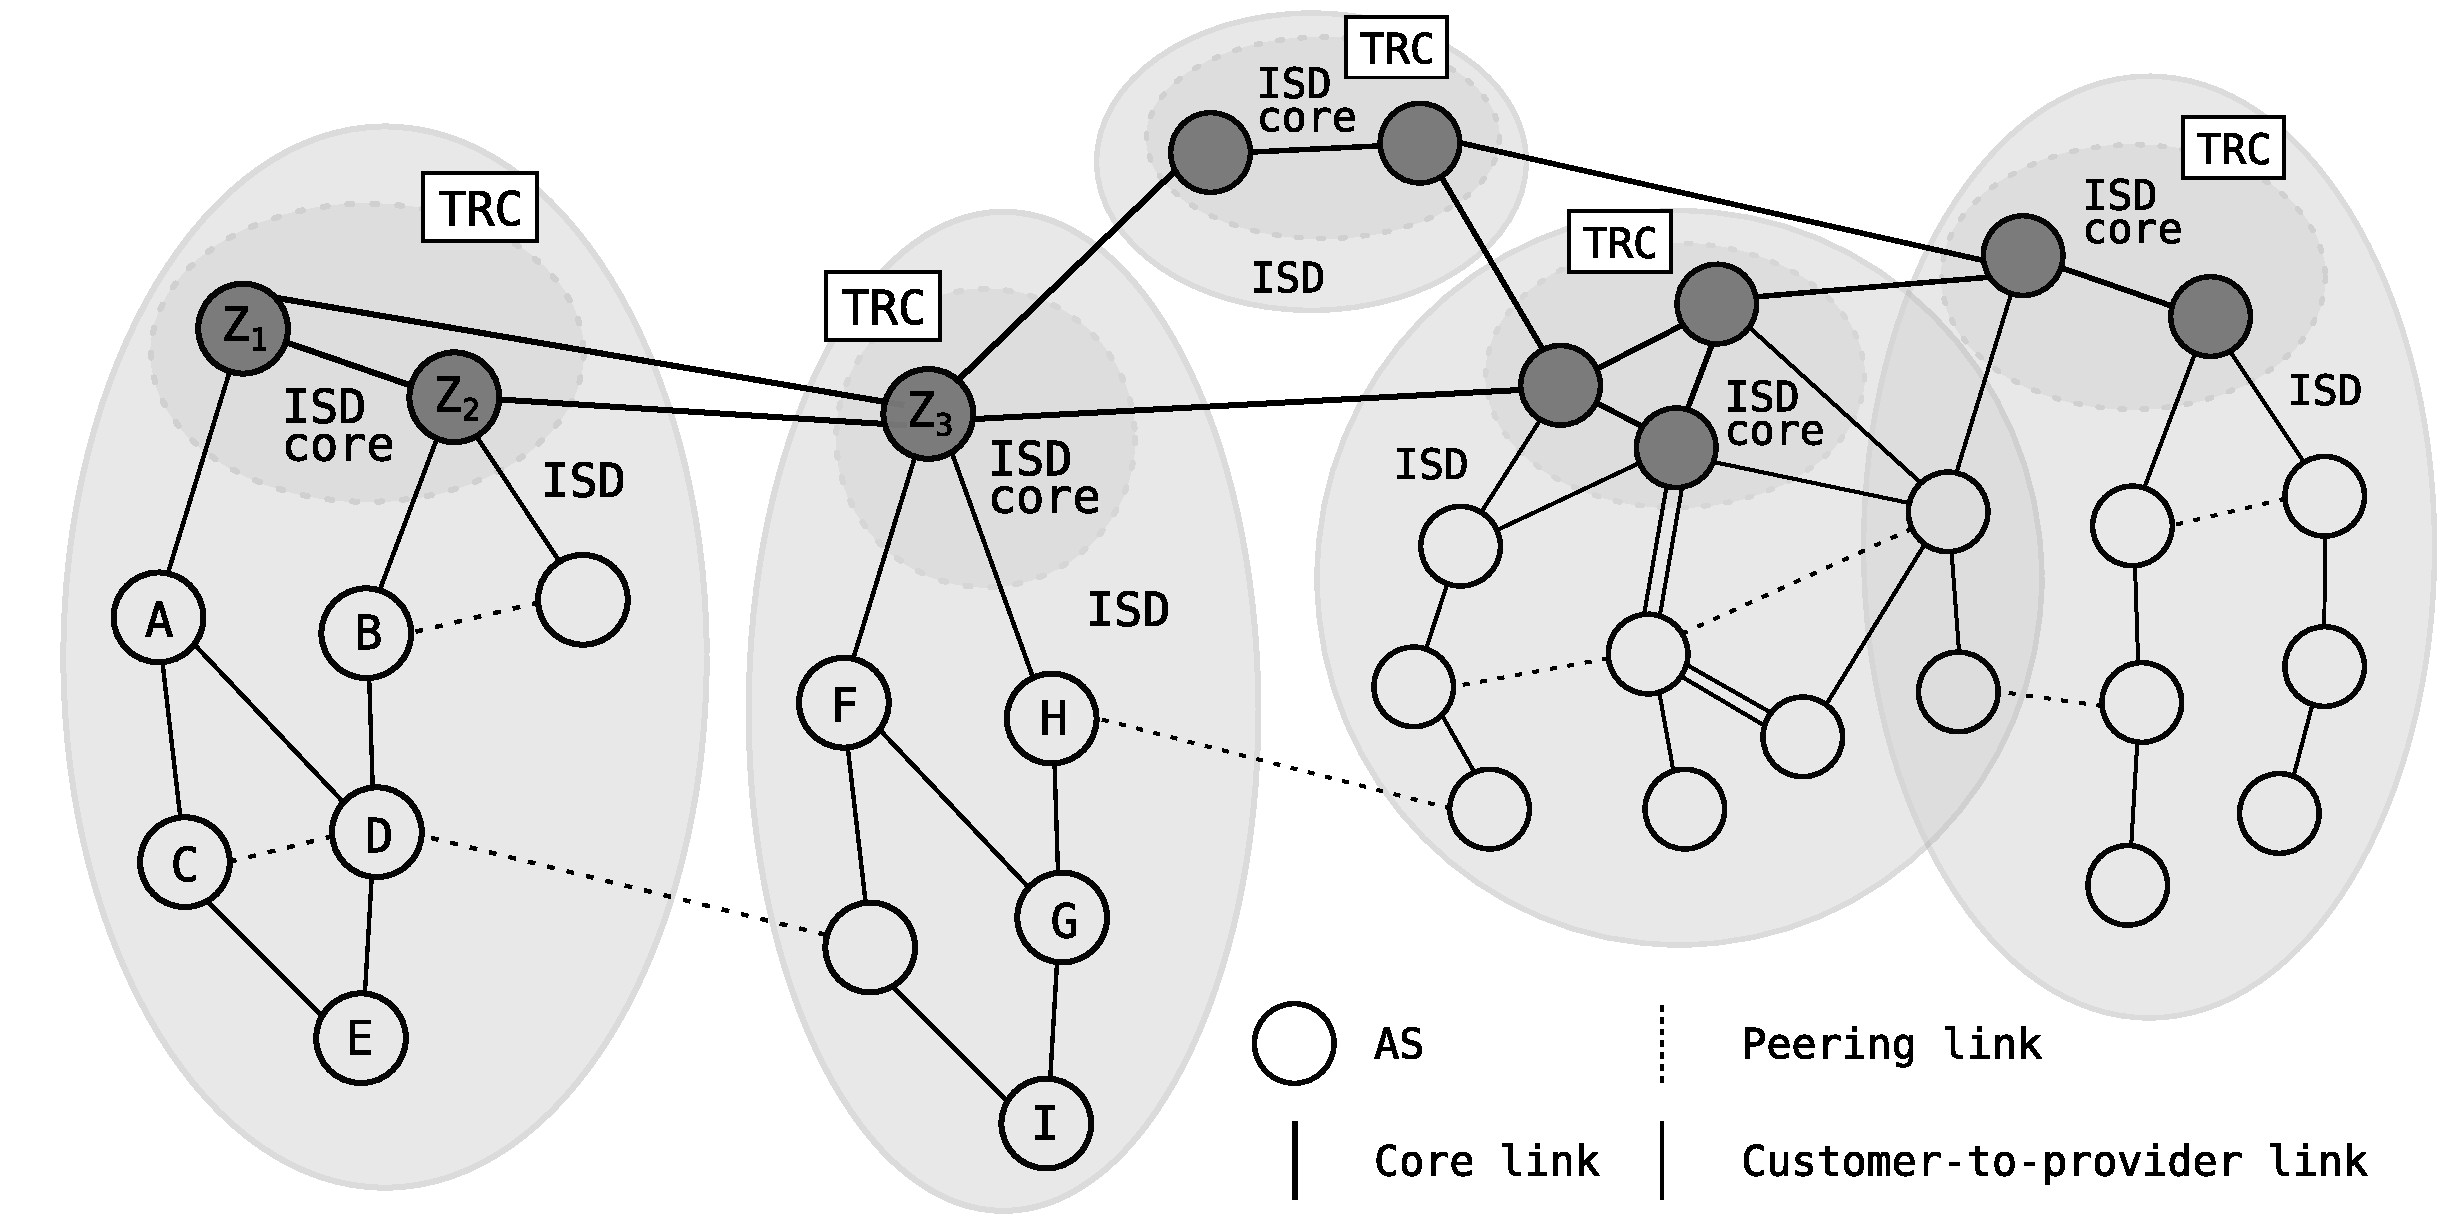
\includegraphics[scale=0.24]{../illustrations/importantConcepts/SCIONISDsAndASes.pdf} 
		\caption[]{Illustration of multiple ISDs with their ASes connected through different types of links. Core ASes via core links and ASes not belonging to the core via customer-to-provider or peering links. This drawing is inspired by the one shown in the SCION book \cite{SCIONBook} on page 18.}
		\label{fig:SCIONArchitectureISDs}
	\end{center}
\end{figure}

To enable an exchange between two endpoints, one or more paths through the network must be defined along which the data is sent. Every single step which is necessary to create such forwarding paths can be assigned to one of two planes. The control plane is responsible for discovering the paths and making them available to the end hosts, whereas the data plane is responsible for forwarding the data along the corresponding paths. This strict separation of routing (control plane) and forwarding (data plane) is one of the key features of SCION. The individual steps of creating a forwarding path are summarized below and illustrated in Figure \ref{fig:SCIONCreationForwardingPath}. The heading of the individual parts indicates their assignment to the corresponding plane.

\paragraph{Path Exploration (Control Plane)}

The first step in creating a forwarding path is path exploration, called beaconing in SCION terminology. The core ASes regularly send path-segment construction beacons (PCBs) to all its neighbors. Upon reception, an AS adds its own information and forwards the PCBs further to its neighbors. This results in a sequence of ASes representing a path through the SCION network. 

\paragraph{Path Registration (Control Plane)}

An AS typically receives several PCB's which describe path segments to different core ASes. It is up to each AS to decide which of the these it wishes to use. In the path registration, an AS registers the paths via which it wishes to be reached. For this purpose, the corresponding paths are registered at the path servers of the ISD, i.e. they are announced and thus available for the formation of forwarding paths. 

\paragraph{Path Lookup (Control Plane)}

If a source host wants to create a connection to a target host, it carries out a path lookup. From the path servers in the network, it receives path segments that can then be combined, as part of the data plane functionality,  into a forwarding path in a final step. 

\paragraph{Path Combination (Data Plane)}

After a host has received individual path segments in the course of the path lookup, it can now combine these into a path to the destination. Depending on where the destination is located, up to three path segments must be combined. If the destination AS is on the path from source AS to its core AS, then one segment is sufficient. If source and destination share only one core AS within the ISD, two segments are necessary, namely one from the source AS to the core AS and one from the core AS to the destination AS. Three path segments are necessary if source and destination are not located in the same ISD. In addition to the path segments connecting the ASes to their core, a segment between the two core ASes is also necessary.

\begin{figure}
	\begin{center}
		\def\svgwidth{1\textwidth}
		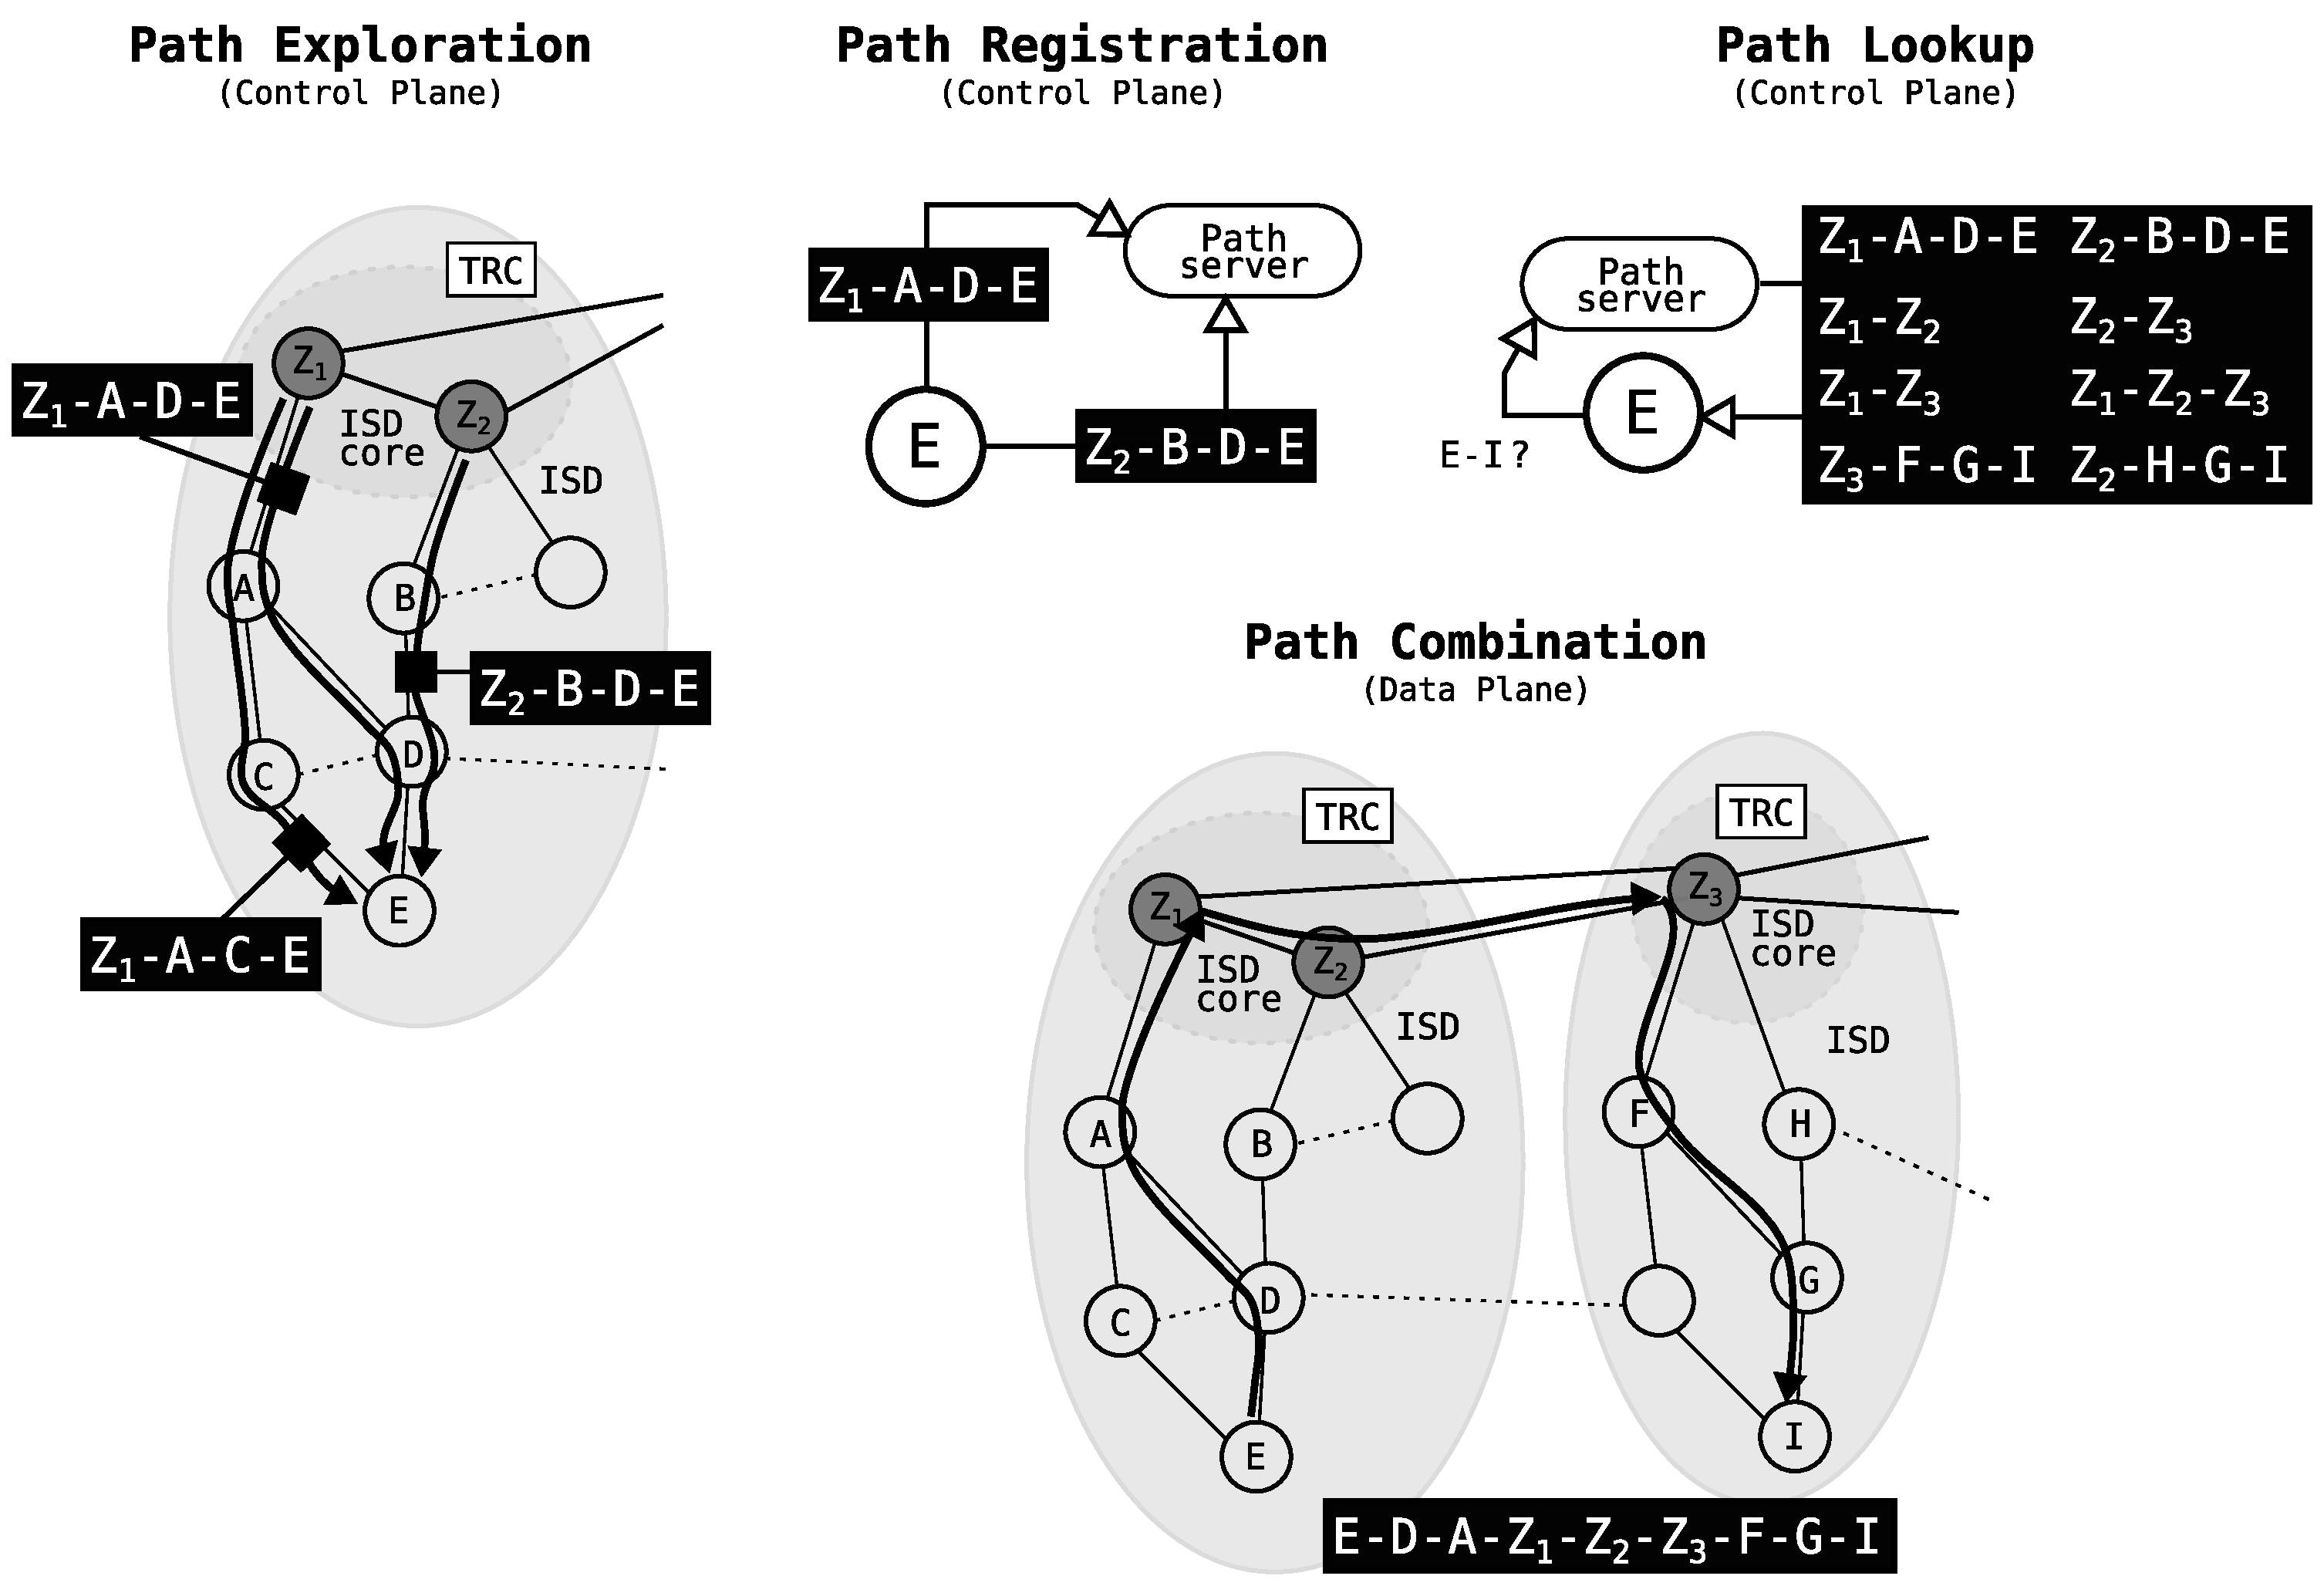
\includegraphics[scale=0.24]{../illustrations/importantConcepts/SCIONPathCreation.pdf} 
		\caption[]{Illustration of the different steps involved in the creation of a forwarding path: During path exploration, the AS E receives three PCB's describing different paths to reach the core. It decides to register two of these at the path server. If AS E wants to reach AS I it performs a lookup at the path server to get possible path segments. These individual path segments can then in the path combination be arbitrarily joined to form a forwarding path used for data exchange.}
		\label{fig:SCIONCreationForwardingPath}
	\end{center}
\end{figure}

\paragraph{Forwarding (Data Plane)}

Once a path is formed, it is included in the SCION packet header and used for forwarding. The recipient of a packet can send back data by simply inverting the path along which it got the packet or create a different one by performing a path lookup and combination on its own.

\subsection*{Conclusion}

This summary only scratches the surface of the functionality that SCION provides. The new i´nternet architecture offers a variety of additional functions, security mechanisms and extensions which are not mentioned here. The goal of this section was to explain why the transformation to a new Internet architecture is so important and to introduce SCION as a promising candidate. Interested readers are again referred to the SCION book \cite{SCIONBook} or website \cite{SCIONWebMain}.

\chapter{Shila - Introduction}
\label{chap:ShilaIntroduction}

This chapter introduces the central point of the thesis and the author's main contribution towards the establishment of a more secure internet architecture. A piece of software that allows the usage of MPTCP over SCION. The chapter includes a presentation of the software, an explanation of how to  use it and a rough outline of the functionality under the hood. A detailed discussion of the implementation follows in Chapter \ref{chap:ShilaImplementation}.   

\section{Introduction}
\label{sec:ShilaIntroduction}

Shila could very well be the name of the female lead role in a thrilling crime novel. However, in the context of this work Shila is the abbreviation of shim layer. It appropriately names the implementation which, by mediating between the two technologies, enables the use of MPTCP over SCION.

\subsection*{Initial Situation}
\label{subsec:ShilaInitialSituation}

To simplify the following descriptions, the starting point for the use of Shila is defined. To use Shila, one needs at least two devices\footnote{The usage of multiple instances of Shila on a single device is also possible. For illustrative purposes, however, this scenario is not discussed here.} with MPTCP installed. In addition, the devices must be connected through the SCION network. Guidance to install MPTCP can be found here \cite{MPTCPWebMain}, the setup of SCION is described in detail on the official SCION webpage \cite{SCIONWebMain}.

Each device is identified by a SCION address, not surprisingly referred to as the SCON address of a host. TCP applications, or TCP endpoints, which are executed on a host are bound to a network interface. They are uniquely addressable through an IP address paired with a TCP port number, denoted as TCP address of an application. The individual parts of this tuple are called the IP address or the TCP port of an application. Furthermore, TCP applications can also be linked with addresses of the SCION namespace. The same principle applies here. Thus, an application may also be identified either by a full SCION address or just individual parts of it, e.g. just the SCION port.

\subsection*{Usage}
\label{subsec:ShilaUsage}

In the following, a simple example case describes how a user can utilize Shila. A description on how to use Shila is also part of the Shila code repository \cite{ShilaGithub}.

As an example, a setup with two endpoints is considered. Host 1 with SCION address {\footnotesize 1-ff00:0:112,127.0.0.1} and Host 2 with address {\footnotesize 2-ff00:0:220,127.0.0.1}, both are part of the SCION network. The goal is to establish a connection between the client instance of an TCP application running on Host 1 and the respective server instance with TCP address {\footnotesize 10.7.0.9:27041} running on Host 2. As an example TCP application, we consider iPerf3, the well-known measurement tool.

First, the so-called Routing-Information for the Shila instance running on Host 1 has to be prepared. It describes the mapping between TCP address of an application running on a certain host and the same host's SCION address. The routing information stored in a file named \textit{routing.json} and is located in the Shila root directory. For the given example it contains only one entry:

\begin{minted}
{json}
[{ "key"  : { "ip" : "10.7.0.9", "port" : "27041" },
   "flow" : { "address"  : "2-ff00:0:220,127.0.0.1:27041" } }]
\end{minted}

In the second step, the Shila instance on both hosts can be started. If no arguments are specified the program starts with the default settings and loads the routing entries from the previously mentioned file:
\begin{minted}
{bash}
sudo ./shila
\end{minted}
The server instance of iPerf3 can be started on Host 2 once the shim layer is running. To be reachable, the instance has to be started in the ingress network namespace of Shila:

\begin{minted}
{bash}
sudo ip netns exec shila-ingress iperf3 -s -p 27041
\end{minted}

As final step the client part of iPerf3 is executed in Shilas egress network namespace on Host 1:

\begin{minted}
{bash}
sudo ip netns exec shila-egress iperf3 -c 10.7.0.9 -p 27041
\end{minted}

\newpage
Following, the output of certain involved entities is shown. Figure \ref{fig:IntroductionOutputShilaOnHost1} displays the output generated by the Shila instance running on Host 1. The shim layer creates a default number of three paths through the SCION network used for the data exchange between the two iPerf3 instances. Figure \ref{fig:IntroductionOutputIperfOnHost1} shows the output generated by iPerf3 running on Host 1. Figure \ref{fig:IntroductionDataDistributionAmongPaths} visualizes the distribution of the data exchange among the three different flows.

\begin{figure}
	\begin{center}
		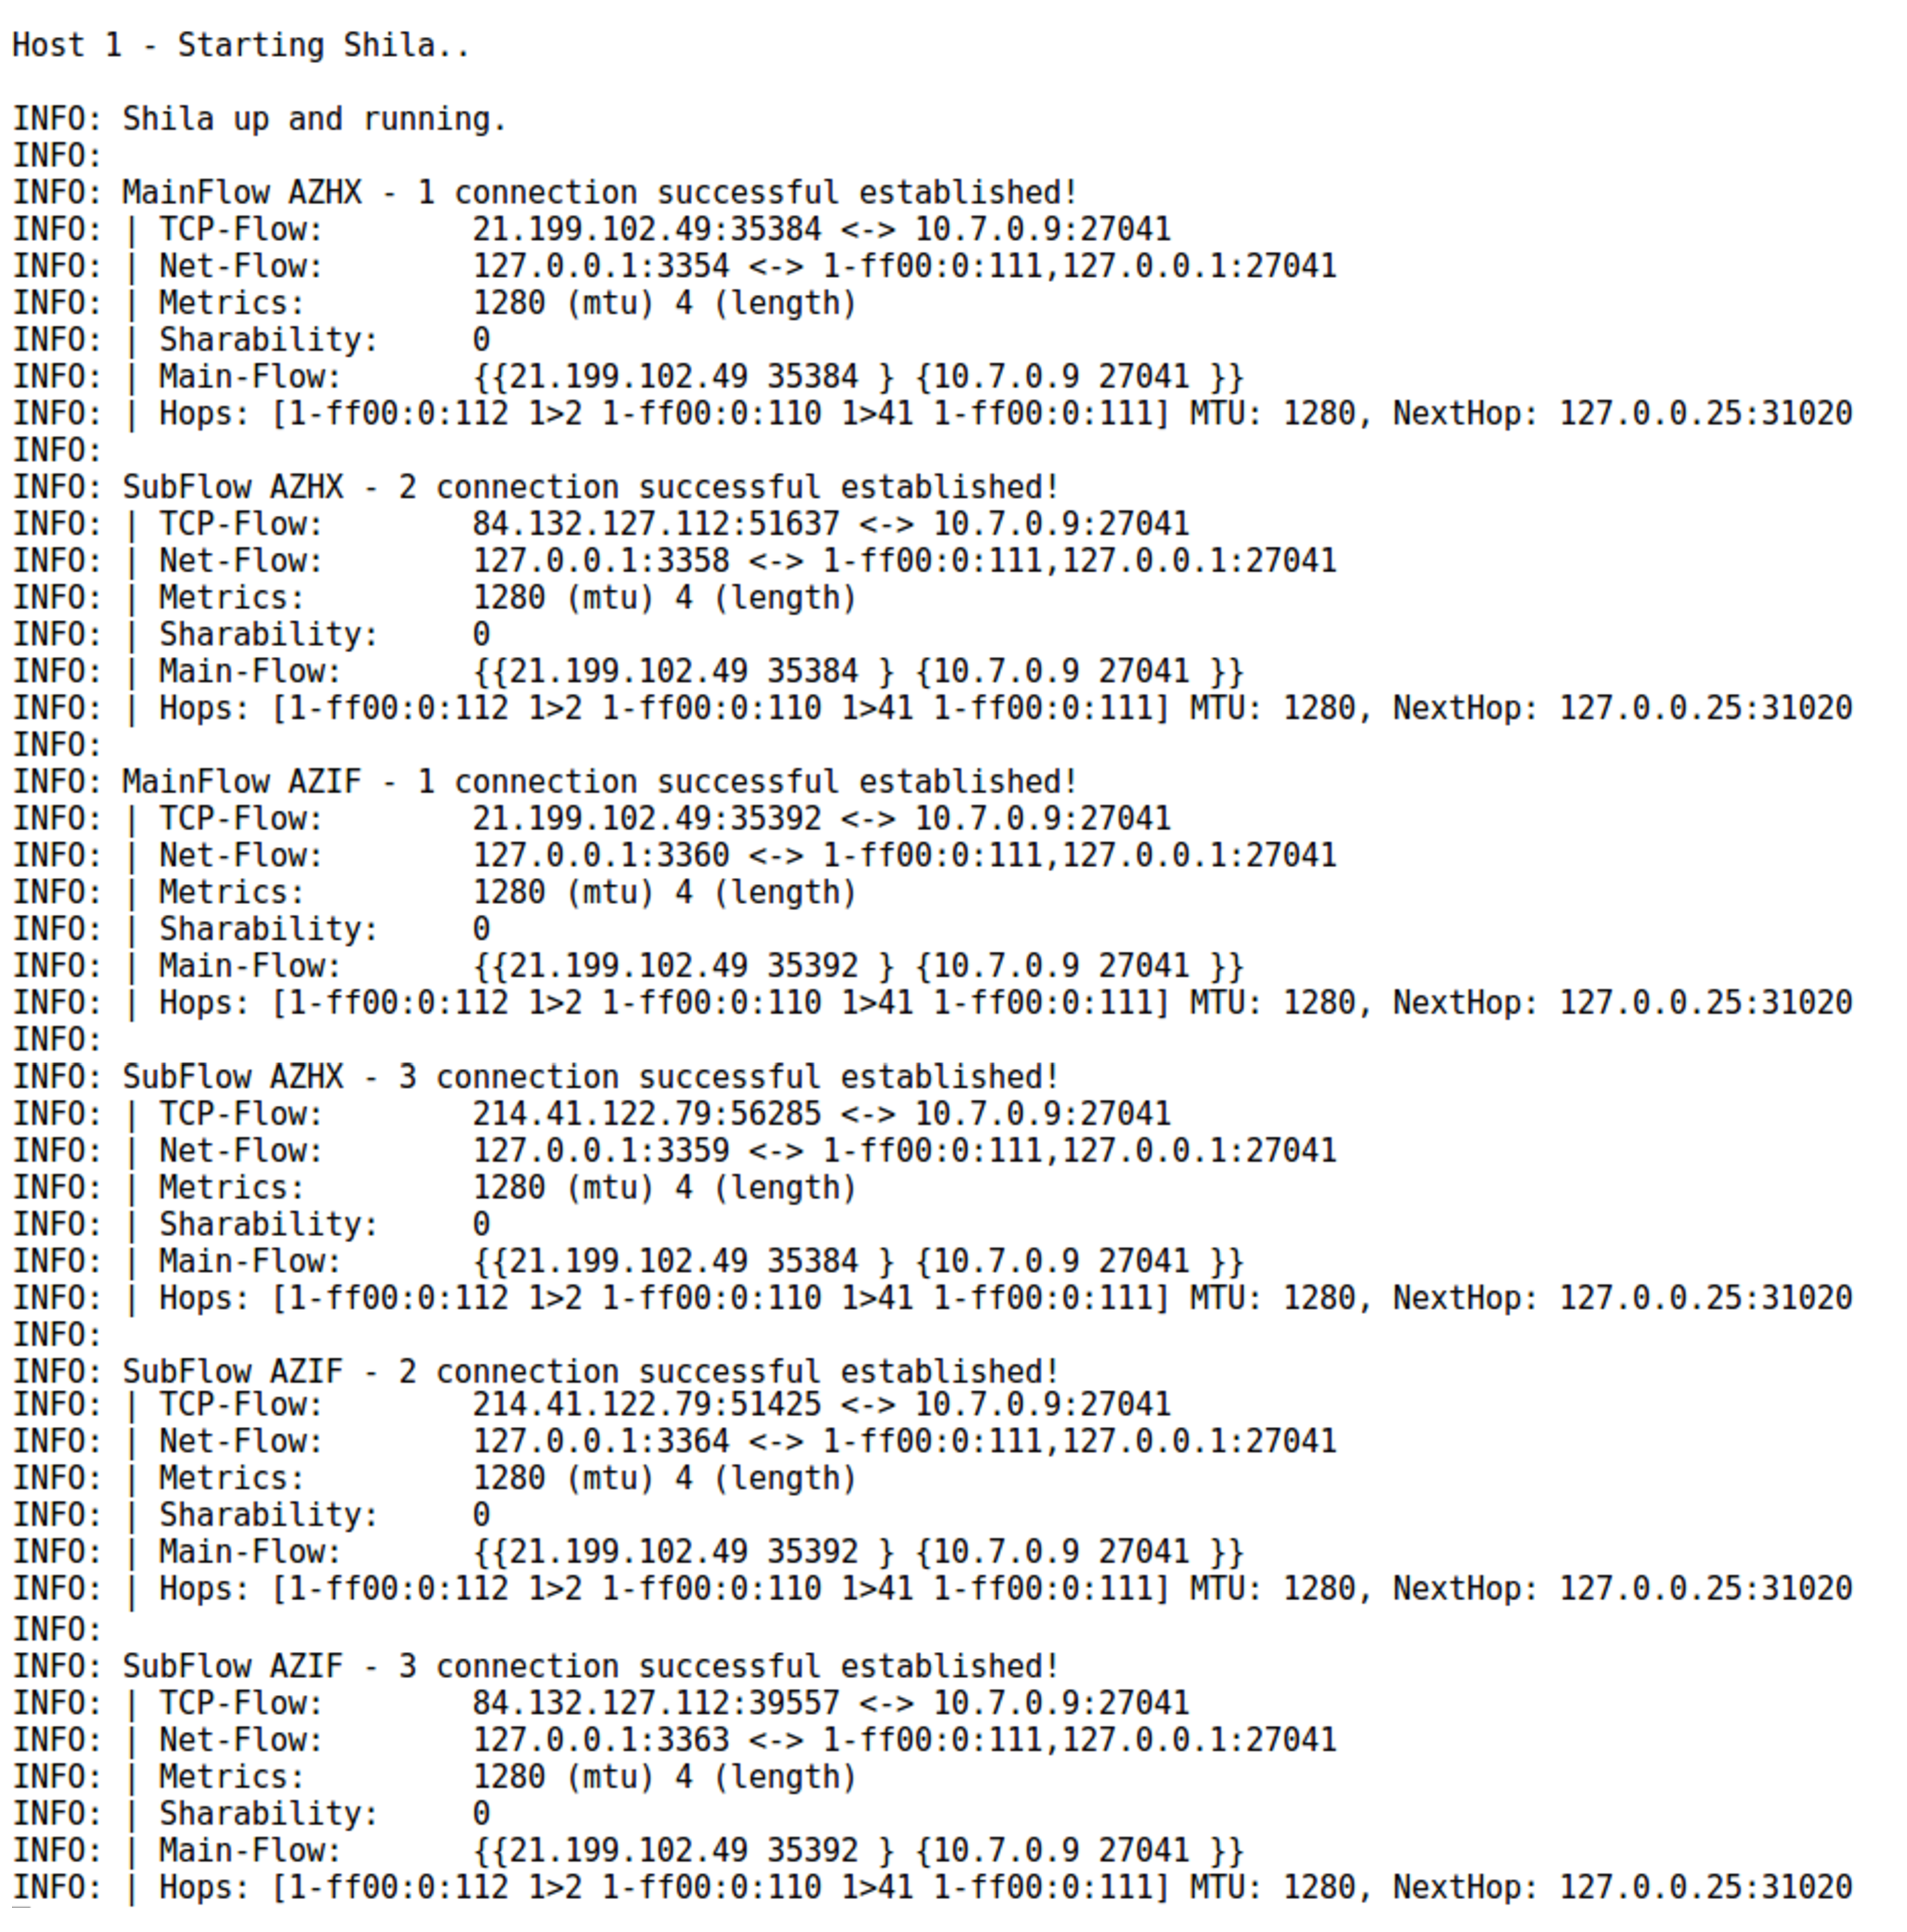
\includegraphics[scale=0.27]{../illustrations/shilaIntroduction/OutputShilaHost1.pdf}  
		\caption[]{Output generated by the Shila instance running on Host 1. Note that iPerf3 creates two TCP connections, one to send the control signals and one for the actual data exchange.}
		\label{fig:IntroductionOutputShilaOnHost1}
	\end{center}
\end{figure}

\begin{figure}
	\begin{center}
		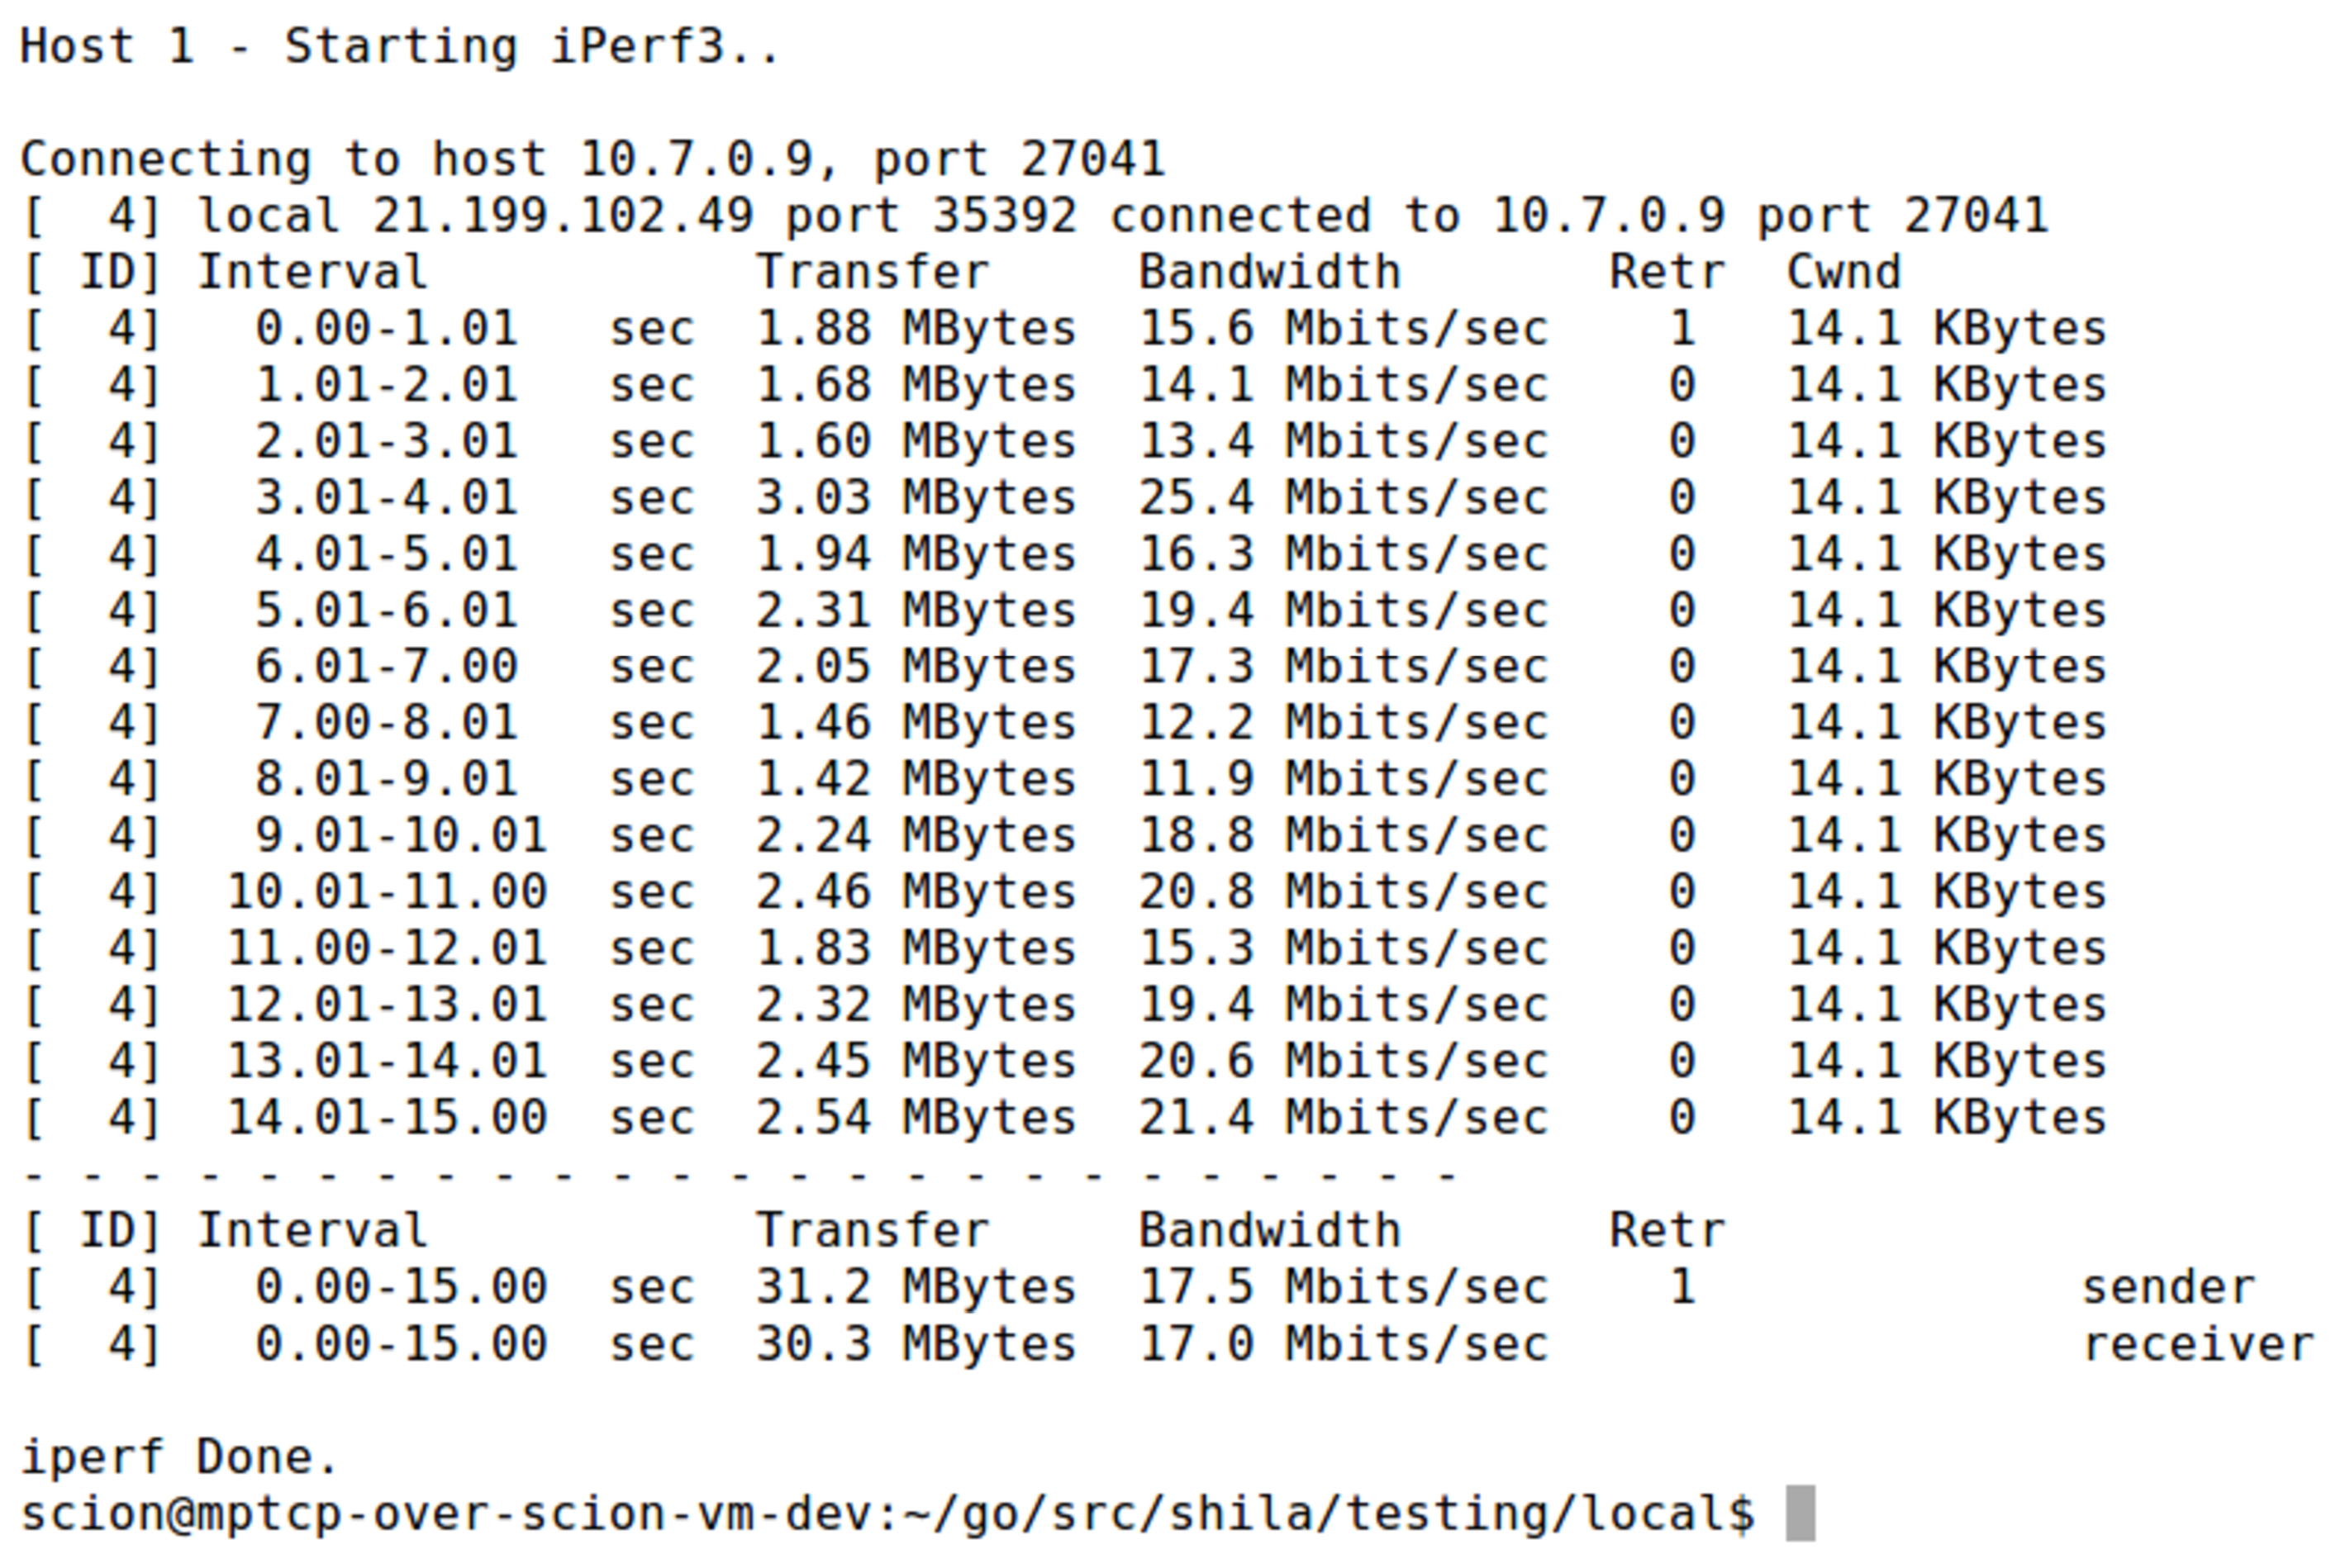
\includegraphics[scale=0.27]{../illustrations/shilaIntroduction/OutputiPerf3Host1.pdf}  
		\caption[]{Output generated by the iPerf3 client instance on Host 1. Note that the measured metrics are not representative since the test run was done on a local setup of SCION.}
		\label{fig:IntroductionOutputIperfOnHost1}
	\end{center}
\end{figure}

\begin{figure}
	\begin{center}
		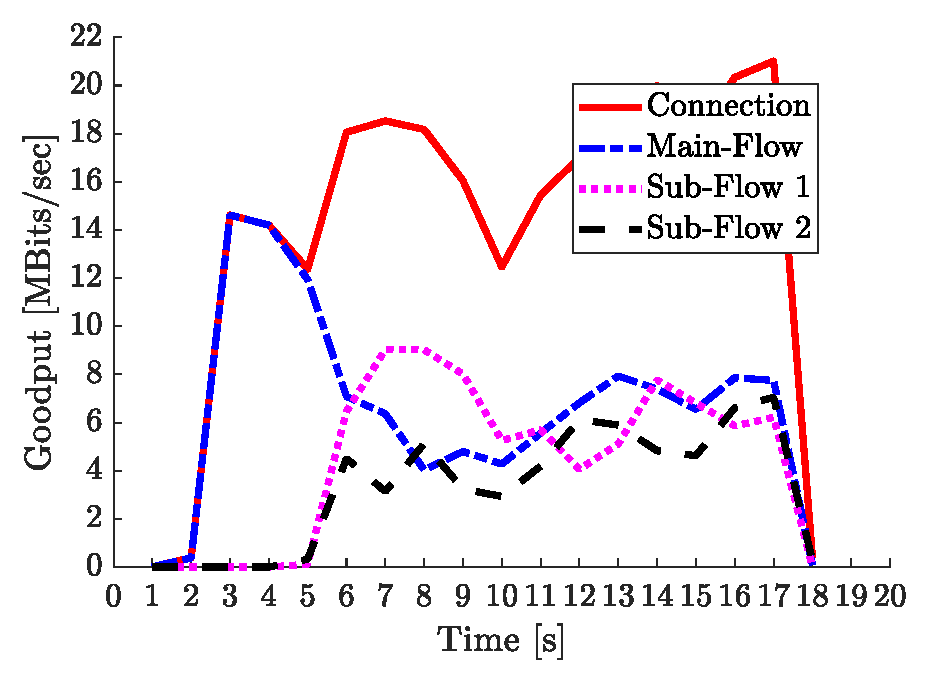
\includegraphics[scale=0.65]{../illustrations/shilaIntroduction/DistributionOfFlows.eps}  
		\caption[]{Plot showing how the achieved goodput for the connection between Host 1 and Host 2 is under hood distributed to the three flows created by Shila.}
		\label{fig:IntroductionDataDistributionAmongPaths}
	\end{center}
\end{figure}


\newpage
\section{Functionality}
\label{sec:ShilaFunctionality}

The functionality of Shila can be divided into three parts. The first part considers the setup of Shila in general, i.e. everything necessary to get a running instance of Shila. The latter two parts specifically consider the data exchange between two TCP endpoints. In detail, the second part discusses what is necessary to establish such a connection and the third part covers the operating state and also the cleaning up once a connection is no longer needed. 

In the following subsections the three parts are outlined, so the reader gets a basic understanding of the mechanics of Shila. In Chapter \ref{chap:ShilaImplementation} everything mentioned is explained again in more detail.

\subsection*{Setup}

Launching and setting up Shila includes the following steps.

\paragraph{Loading of the Routing-Information} Shila reads the Routing-Information presented in the respective file. It contains the mapping from TCP addresses of applications to SCION addresses of hosts running these apps. 

\paragraph{Setup of Namespaces} Shila sets up two different network namespaces. The ingress namespace (\textit{shila-ingress}) holds the network interface used to accept incoming connections. The egress namespace (\textit{shila-egress}) accommodates the network interfaces which are used for connections initiated by the respective host.

\paragraph{Creation of virtual Interfaces} A virtual network interface is a network device that is supported entirely in software, i.e. there is no real hardware network adapter. It allows applications to take over the role of the wire. For a real network interface, the IP datagrams of connected applications are sent directly to the cable. Virtual interfaces make these data available to applications in userspace.

The shim layer instantiates a single virtual network interface in the ingress namespace. This interface is per default bound to the IP address {\footnotesize 10.7.0.9} and is used by all listening TCP applications to bind their sockets. In the egress namespace one to eight\footnote{The current implementation of MPTCP uses a maximum of eight different interfaces for a single MPTCP connection.} virtual interfaces can be instantiated. Each is assigned a random IP address. Each of these virtual network interfaces later corresponds to a single flow of an MPTCP connection.

\paragraph{Running the Contact-Server-Endpoint} To be receptive to incoming connections, Shila starts a so-called Contact-Server-Endpoint. It binds per default to the SCION port {\footnotesize 7654} and serves as an initial point of contact. Shila instances running on different hosts initiate possible data exchange through this contact point.

\begin{figure}
	\begin{center}
		\def\svgwidth{1\textwidth}
		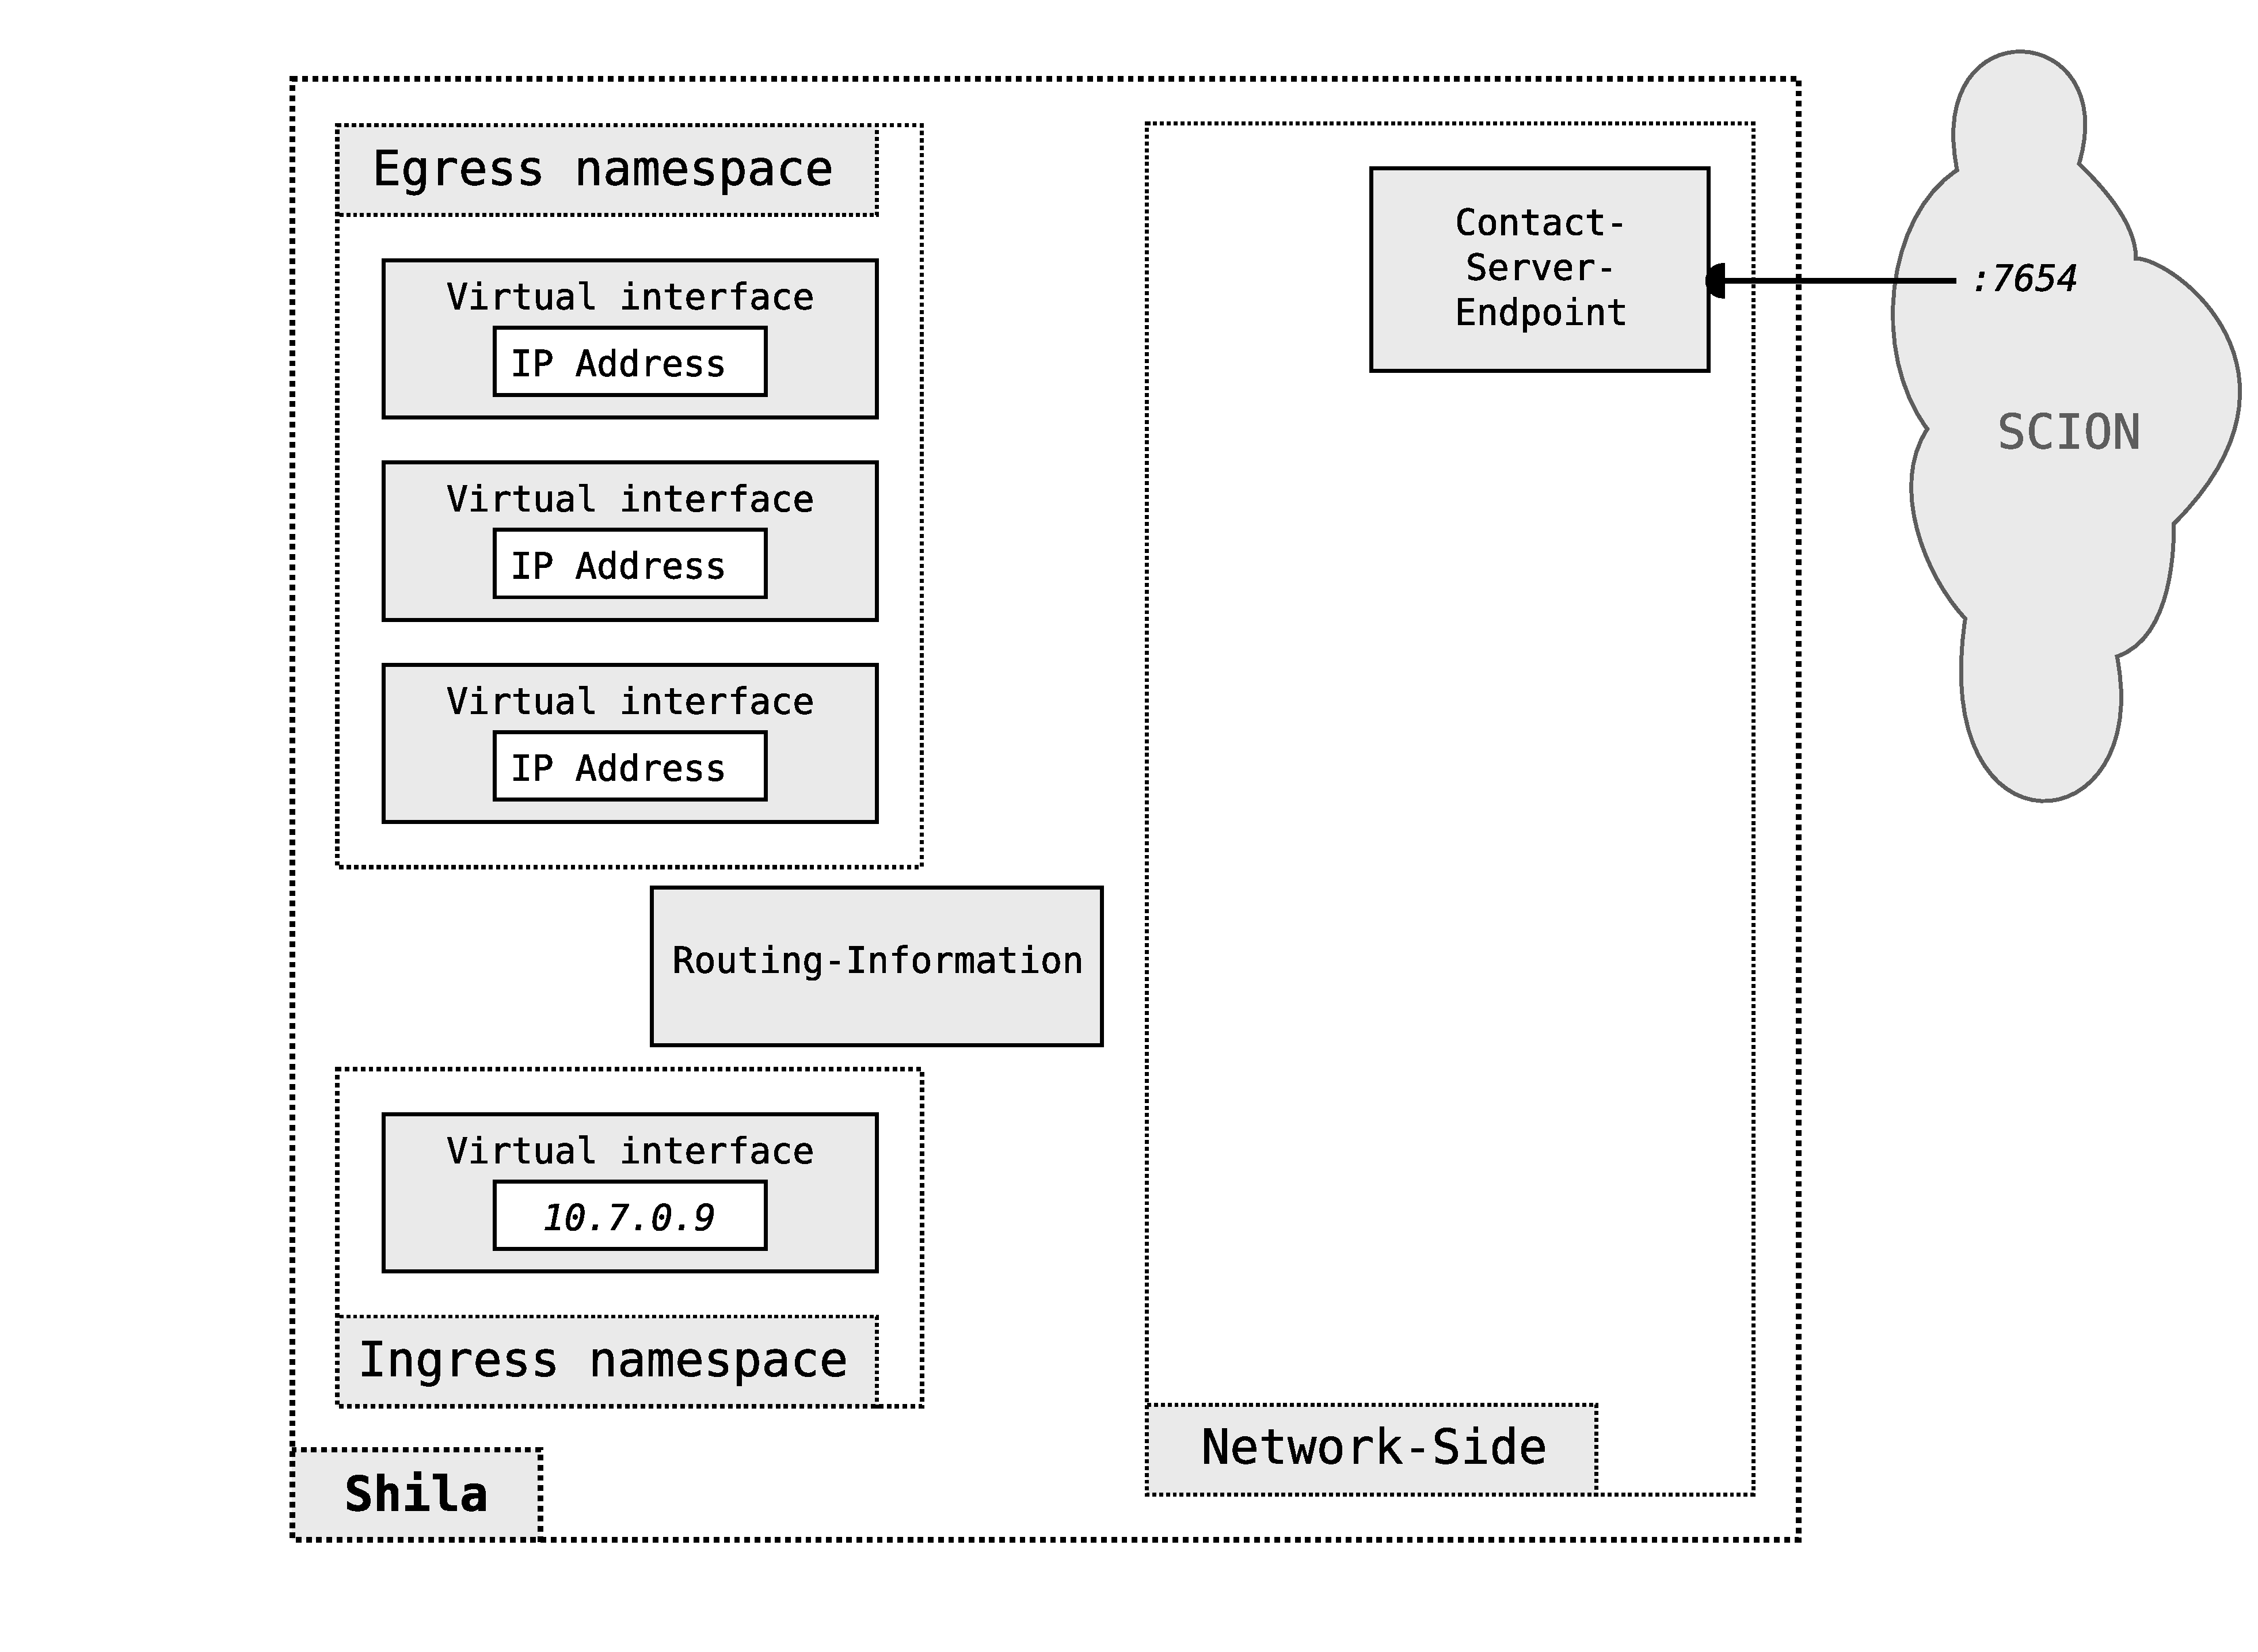
\includegraphics[scale=0.2]{../illustrations/shilaIntroduction/StateAfterSetup.pdf}   
		\caption[]{Illustration of the state of Shila once the setup is complete. Through the Contact-Server-Endpoint, Shila receives connection requests from other instances. Applications (server) can bind to the virtual interface in the ingress namespace. Requests from applications (client) are intercepted by Shila via the virtual interfaces in the egress namespace.}
		\label{fig:ShilaIllustrationStateAfterSetup}
	\end{center}
\end{figure}

Figure \ref{fig:ShilaIllustrationStateAfterSetup} illustrates the state of Shila once the setup is completed. The implementation is now ready to establish connections and provide data exchange between the client and server instance of TCP applications running on, possibly different, SCION hosts. 

\subsection*{Connection Establishment}
\label{subsec:ShilaConnectionEstablishment}

This subsection presents the individual steps of a connection establishment between a client instance of an application and its server counterpart over MPTCP on top of SCION. The discussion is based on the example of Subsection \ref{subsec:ShilaUsage} and it assumes that a successfully initialized instance of Shila is running on Host 1 and Host 2. All the presented steps are illustrated in Figure \ref{fig:ShilaIllustrationConnectionEstablishment}. 

\begin{figure}
	\begin{center}
		\def\svgwidth{1\textwidth}
		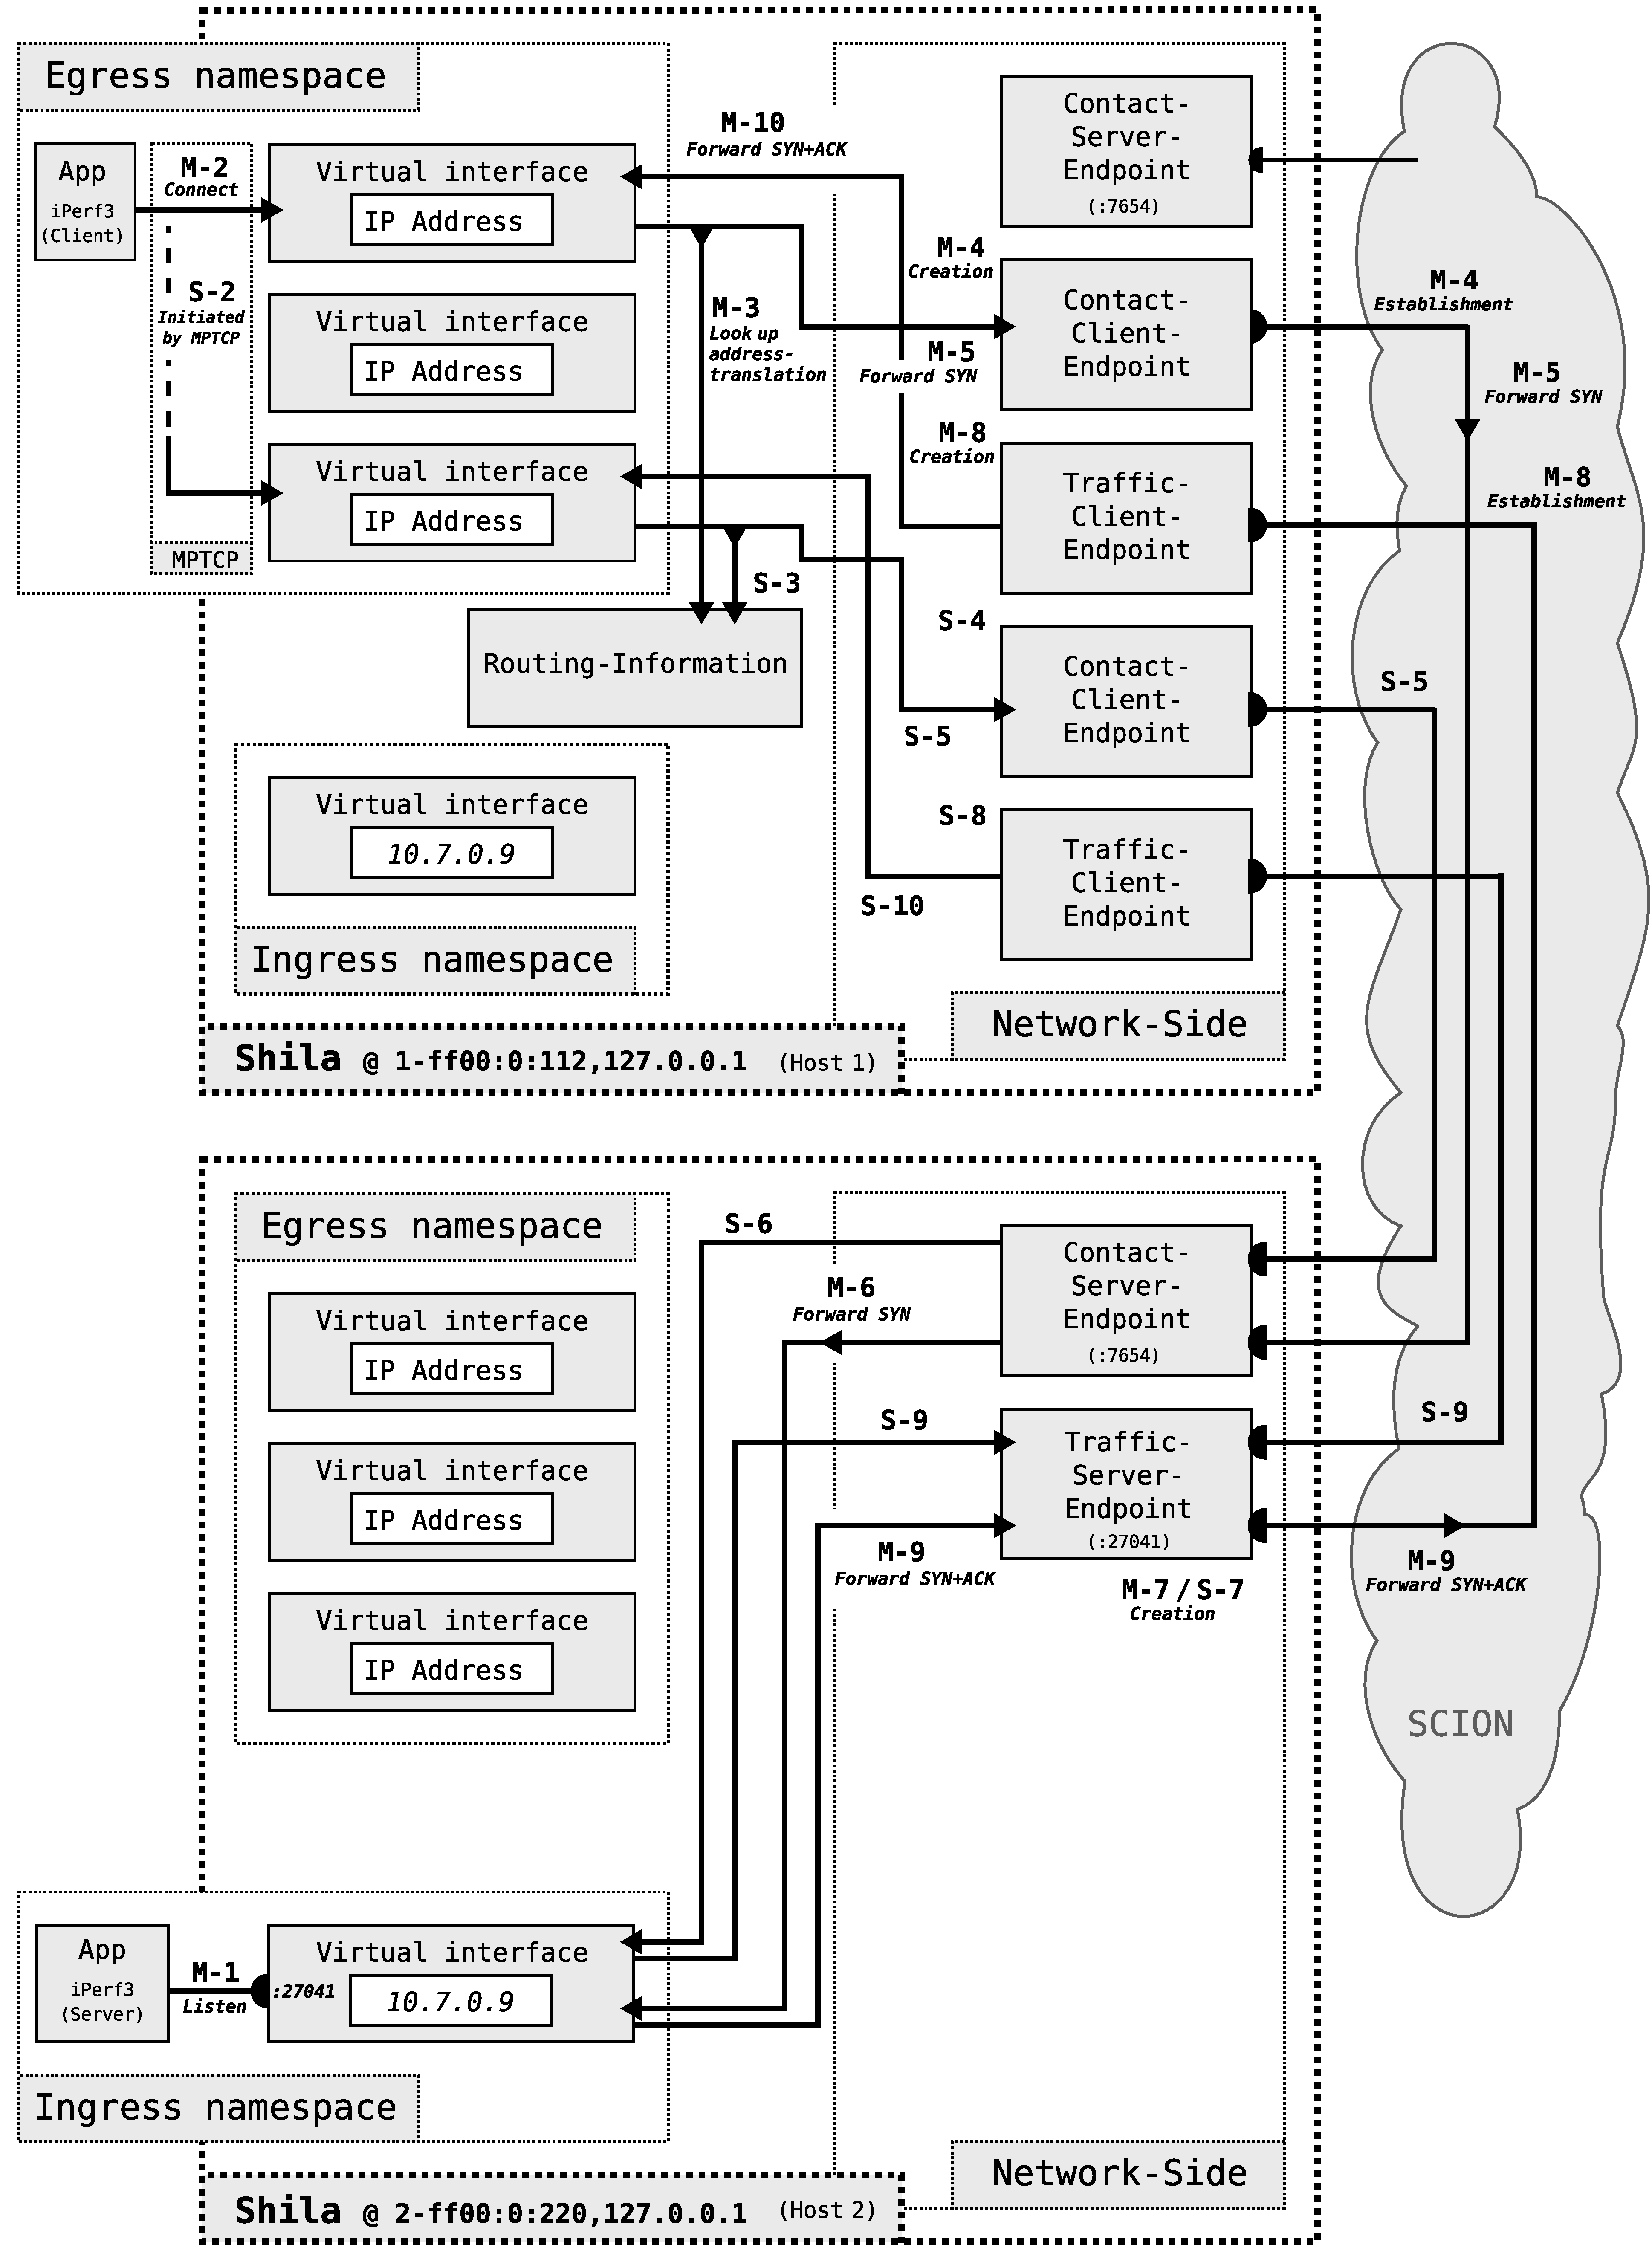
\includegraphics[scale=0.2]{../illustrations/shilaIntroduction/ConnectionEstablishment.pdf}   
		\caption[]{Illustration of the steps involved in the connection establishment of a Main-Flow (\textbf{M-1} to \textbf{M-10}) and a Sub-Flow (\textbf{S-1} to \textbf{S-10}).}
		\label{fig:ShilaIllustrationConnectionEstablishment}
	\end{center}
\end{figure}

The creation of a connection itself can be divided into two parts. The establishment of the initial TCP connection, also called Main-Flow, and the establishment of further TCP connections, the so-called Sub-Flows. For all upcoming parts of this thesis a connection always means the totality of all flows, i.e. the Main-Flow and all possible Sub-Flows. Next, a walk-through guides through the sequence of steps of a Main-Flow establishment.

\textbf{Main-Flow Establishment}

\begin{description}
	\item[M-1] On Host 2, the server instance of iPerf3 starts listening for incoming TCP connections. It therefore binds to the virtual interface in the Shila ingress namespace on the TCP address {\footnotesize 10.7.0.9:27041}. This step is not recognized by Shila.
	\item[M-2] On Host 1, the client instance of iPerf3 tries to connect to its server counterpart on TCP address {\footnotesize 10.7.0.9:27041}. For the connection establishment an IP datagram, containing the SYN, is sent via one of the virtual interfaces in the egress namespace where it is intercepted by Shila.
	\item[M-3] Shila extracts the destination TCP address from this datagram and looks up the corresponding SCION address in the Routing-Information. For the example, this is {\footnotesize 2-ff00:0:220,127.0.0.1}, the SCION address of Host 2. 
	\item[M-4] A Contact-Client-Endpoint is created. It establishes a backbone connection, called Contact-Backbone-Connection, over SCION to the Contact-Server-Endpoint listening on Host 2, SCION port {\footnotesize 7654}.
	\item[M-5] The SYN is forwarded to the server along the Contact-Backbone-Connection.
	\item[M-6] The Shila instance on the server-side hands over the received IP datagram, holding the SYN, to the virtual network interface in the ingress namespace. From there the datagram finds its destination, the iPerf3 server instance.
	\item[M-7] On Host 2, a Traffic-Server-Endpoint, listening on SCION port {\footnotesize 27041}, is created, ready to receive backbone connections.
	\item[M-8] On Host 1, a Traffic-Client-Endpoint is created. It establishes a so-called Traffic-Backbone-Connection to its counterpart on the server-side.
	\item[M-9] The IP datagram containing the answer from the iPerf3 server instance, a SYN+ACK, arrives at the Shila instance on Host 2. It is forwarded to the corresponding Traffic-Server-Endpoint. From there it is sent over the Traffic-Backbone-Connection to Host 1.
	\item[M-10] The reception of the first data received from the Traffic-Client-Endpoint on Host 1 concludes the establishment of the Main-Flow. Shila extracts its identifier, denoted as Main-Flow-Identifier, and links it to the corresponding routing information. This mapping is important for the following creation of Sub-Flows. The IP datagram, holding the SYN+ACK, is finally handed to the virtual interface from where the initial SYN came from. From there it finds its way to the client instance of iPerf3.
\end{description}

As soon as the Main-Flow of a connection is established, MPTCP starts to initiate Sub-Flows. The procedure differs only in some points from the procedure for establishing a Main-Flow. These points are mentioned below. For illustration purposes, an established Sub-Flow is indicated in Figure \ref{fig:ShilaIllustrationConnectionEstablishment}.

\textbf{Sub-Flow Establishment}

\begin{description}
	\item[(S-1)] This step is not necessary, the server-side of the app is still listening.
	\item[S-2] The initial connection request for a Sub-Flow is not made by the client instance of the application but by MPTCP itself.
	\item[S-3] For a Sub-Flow, Shila extracts the identifier for the corresponding Main-Flow, i.e. the Main-Flow-Identifier, which is carried in the  SYN datagram. It uses this identifier to get all the necessary information about the connection, e.g. the SCION destination address, from the Routing-Information.
	\item[S-7] For a Sub-Flow it is not necessary to create a new Traffic-Server-Endpoint which listens on SCION port {\footnotesize 27041}. Such an instance was already created during the establishment of the corresponding Main-Flow.
\end{description} 

Once established, a flow is immediately used for the data exchange of the application. If at one point the connection is no longer needed, it is removed again, as mentioned in the following subsection.

\subsection*{Normal Operation and Clean-up}
\label{subsec:ShilaCleanUp}

As soon as the Main-Flow or a Sub-Flow is established, its Contact-Backbone-Connection is no longer needed and is terminated. For data exchange between the TCP endpoints, data can be forwarded through all established flows. The decision along which flow the data is sent, is made by MPTCP and cannot be influenced by Shila\footnote{But of course, could Shila decided to send a flow through the Backbone-Connection of a different flow.}. Data forwarded along a certain flow travels via the respective endpoints along the Traffic-Backbone-Connection through the SCION network.  If a connection is no longer needed, i.e. no more data is flowing through, the respective Traffic-Backbone-Connections are removed together with its endpoints.

\chapter{Shila - Implementation}
\label{chap:ShilaImplementation}

In this chapter, we present a more detailed treatise of the implementation of Shila. It builds on the explanations given in Chapter \ref{chap:ShilaIntroduction}, to read it first is therefore recommended. First, an introduction of important terms and concepts is given followed by the description of the underlying implementation structure. Then we treat the three parts of functionality (setup, connection establishment and the normal operation) for a second time, but more detailed than in Chapter \ref{chap:ShilaIntroduction} and with reference to the structure.

\section{Core Concepts and Terms}

Some important concepts and terms are explained below. These are important for further understanding of this chapter. Figure \ref{fig:IllustrationShilaPacket} summarizes them in an illustration.

\subsection{Flows}
\label{subsec:ShilaImplementationImportantConceptsFlows}

The implementation of Shila knows two types of so-called flows; the TCP-Flow and the Net-Flow.  These flows are used to uniquely identify connections and enable internal mapping tasks.

\subsubsection*{TCP-Flow}

The TCP-Flow consists of two TCP addresses representing the connection between two TCP endpoints. One of the two addresses is identified to be the source, the other to be the destination of the TCP-Flow. If used to identify a connection within an endpoint itself, then this endpoint is always the source of the TCP-Flow. Within data that is exchanged from one endpoint (source) to another (destination), the assignment is accordingly.

\subsubsection*{Net-Flow}

The Net-Flow consists of two SCION addresses that represent the connection between two SCION endpoints. The same principles apply here as for the TCP-Flow presented above. In addition to the source and destination, the Net-Flow also contains the SCION path of the corresponding connection.

\subsection{Shila-Endpoint}

A Shila endpoint is a point of contact between Shila and the outside world through which data is received or sent. The different types of these endpoints will be presented in the course of this chapter. To avoid confusion with the naming, the hierarchy of the individual endpoints is listed below.
\\
\dirtree{%
	.1 Shila-Endpoint.
	.2 Kernel-Endpoint.
	.2 Network-Endpoint.
	.3 Client-Endpoint.
	.4 Contact-Client-Endpoint.
	.4 Traffic-Client-Endpoint.
	.3 Server-Endpoint.
	.4 Contact-Server-Endpoint.
	.4 Traffic-Server-Endpoint.
}

\subsection{Shila-Packet}

For the exchange of data so-called Shila-Packets are used. A packet contains the actual payload, namely the IP datagram exchanged between two TCP endpoints. It furthermore holds a link to its creating Shila-Endpoint and is associated with a TCP-Flow as well as Net-Flow. 

\begin{figure}[H]
	\begin{center}
		\def\svgwidth{1\textwidth}
		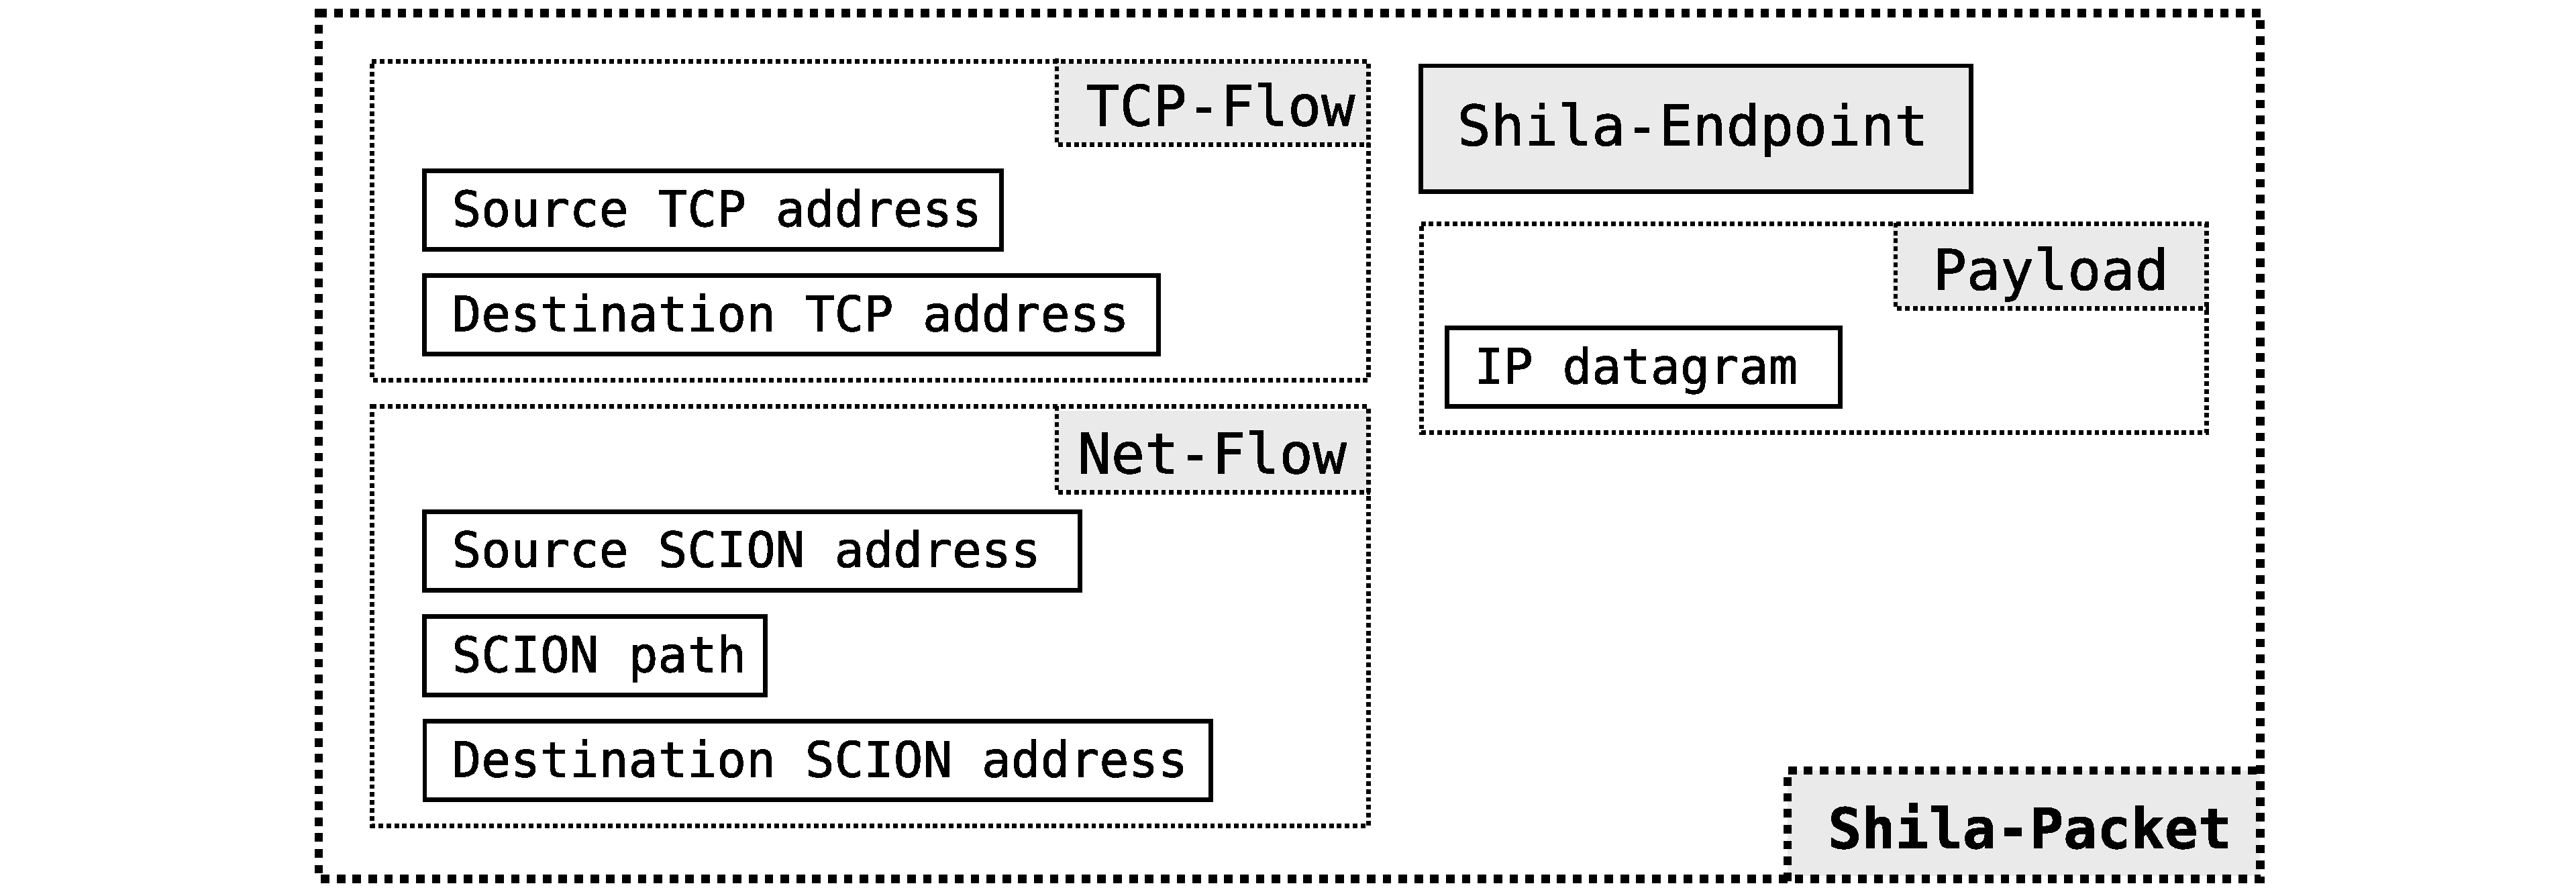
\includegraphics[scale=0.2]{../illustrations/implementation/ShilaPacket.pdf}   
		\caption[Caption for the list of figures.]{Illustration of the Shila-Packet containing the payload, a handle to its creating Shila-Endpoint and the associated TCP-Flow and Net-Flow.}
		\label{fig:IllustrationShilaPacket}
	\end{center}
\end{figure}

\newpage
\section{Structure}
\label{sec:ImplementationStructure}

In the outermost level, the implementation of Shila can be divided into five different parts, illustrated in Figure \ref{fig:ImplementationModulesOutermost}. The Kernel-Side handles the creation of and the interaction with the virtual interfaces and handles the data exchange with the TCP applications. The Network-Side is responsible for the creation and handling of backbone connections over SCION and the data exchange with Shila instances on other computers. The Working-Side in between receives incoming data from both sides and makes sure that it is handed over to the correct Shila-Connection. The Shila-Connection itself maintains the state of a connection and delivers the data to the desired destination. To be able to do this, the Shila-Connection relies on the services of the Router.  The data exchange between the individual parts takes place via traffic channels, transporting the Shila-Packets. In the following, we discuss each of the parts in more detail and provide a more detailed subdivision of the structure into further subparts and their functionality.  

\begin{figure}[H]
	\begin{center}
		\def\svgwidth{1\textwidth}
		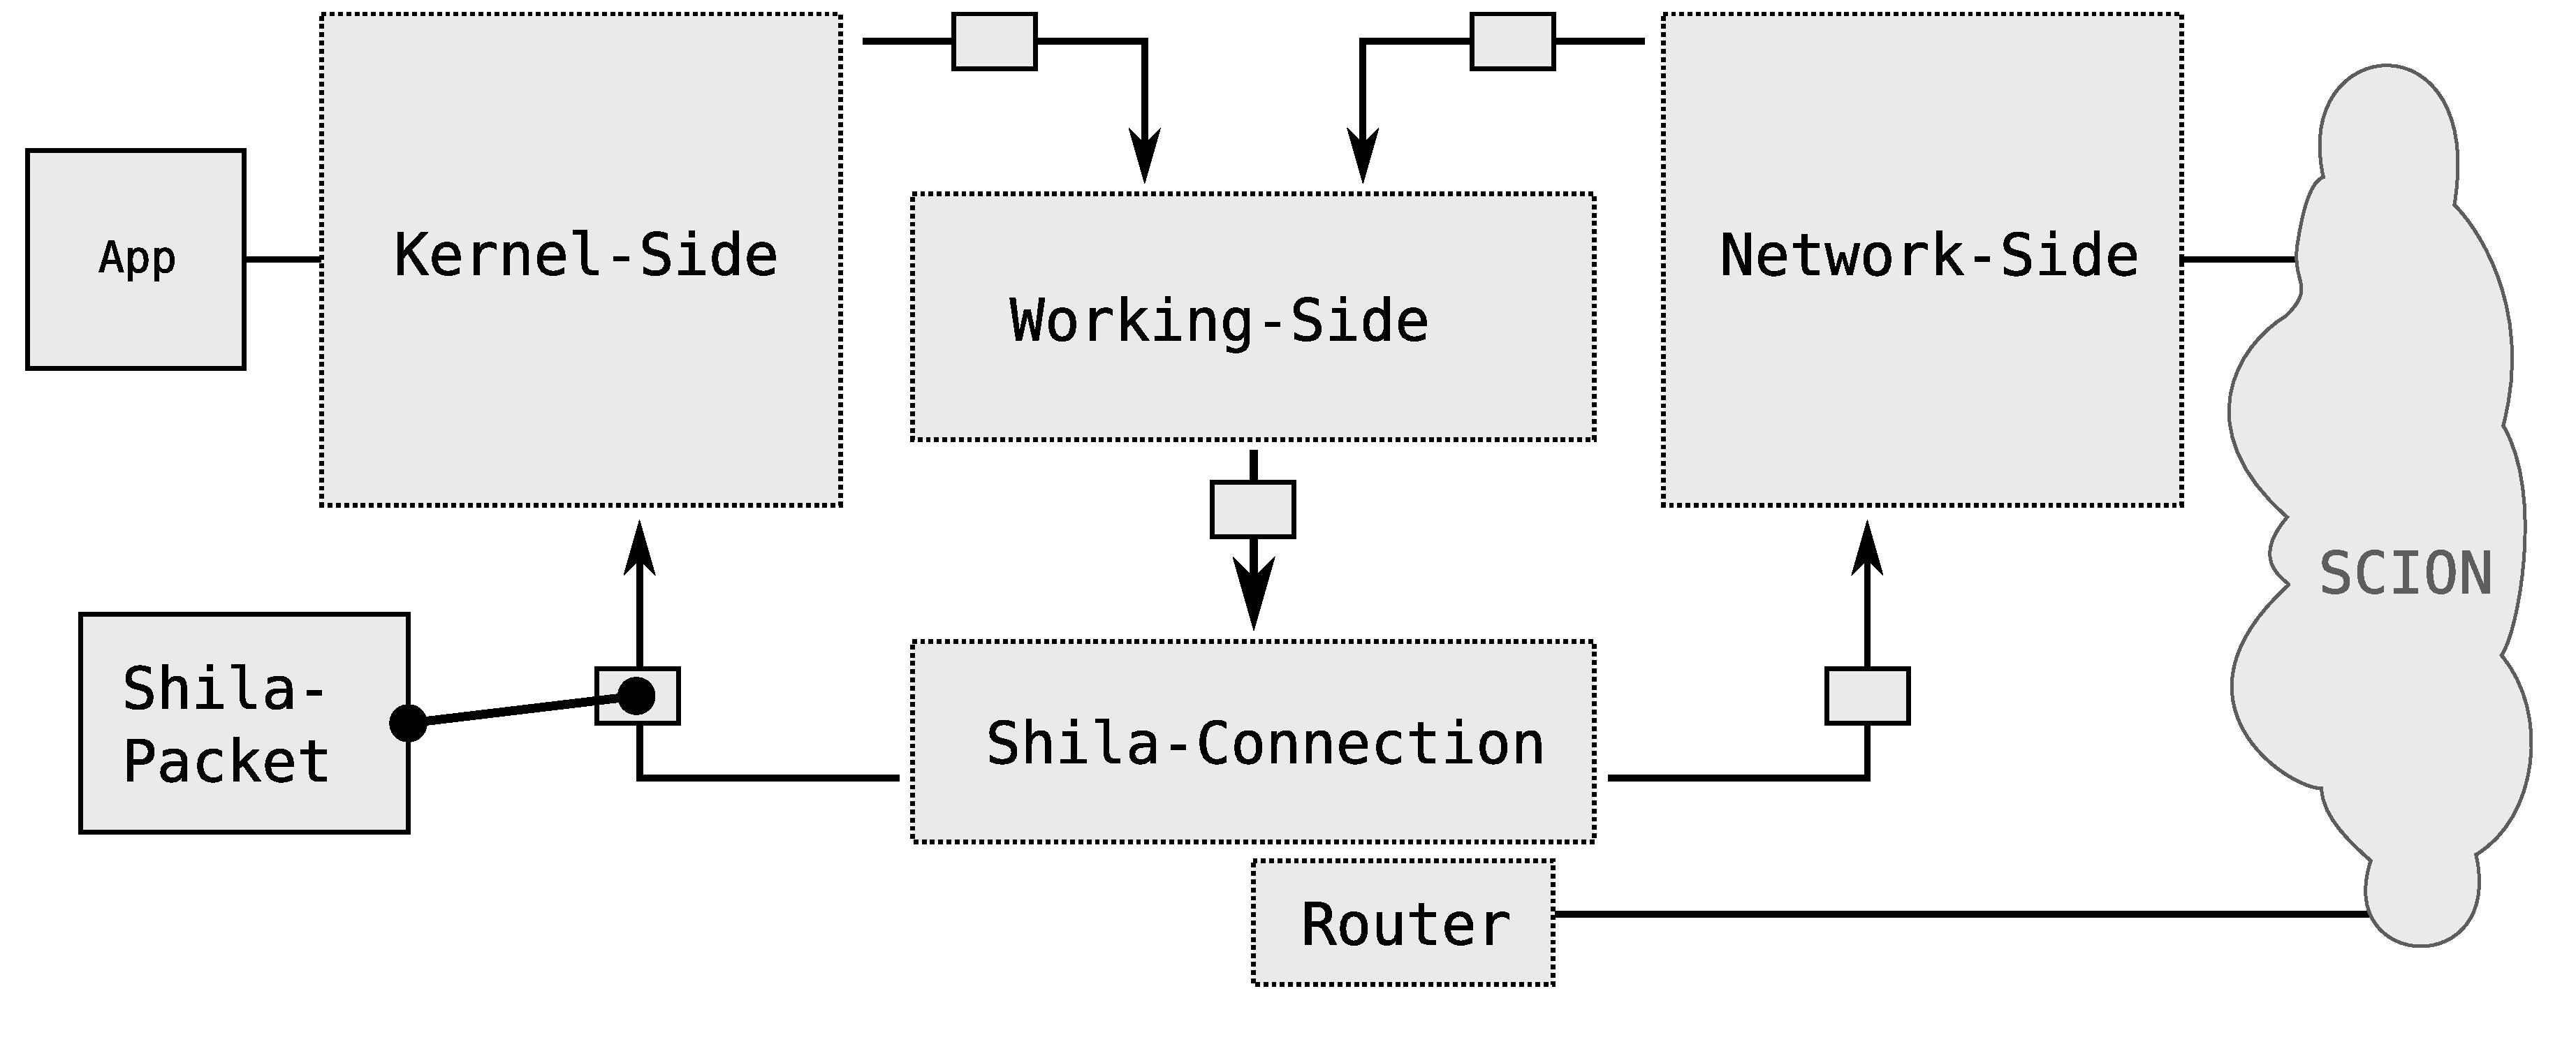
\includegraphics[scale=0.2]{../illustrations/implementation/ModulesOutermost.pdf}   
		\caption[Caption for the list of figures.]{Illustration of the outermost division of the implementation into different parts.}
		\label{fig:ImplementationModulesOutermost}
	\end{center}
\end{figure}

\subsection{Kernel-Side}

The Kernel-Side, shown in Figure \ref{fig:ImplementationModulesKernelSide}, is managed by an appropriate manager, allocating the network namespaces and creating the individual Kernel-Endpoints, which are located within the namespaces. It furthermore provides an interface for the creation of Kernel-Endpoints and it allows to query for the traffic channels held by these endpoints. The Kernel-Endpoint-Mapping stores a mapping from IP addresses to the corresponding Kernel-Endpoints.  

\begin{figure}
	\begin{center}
		\def\svgwidth{1\textwidth}
		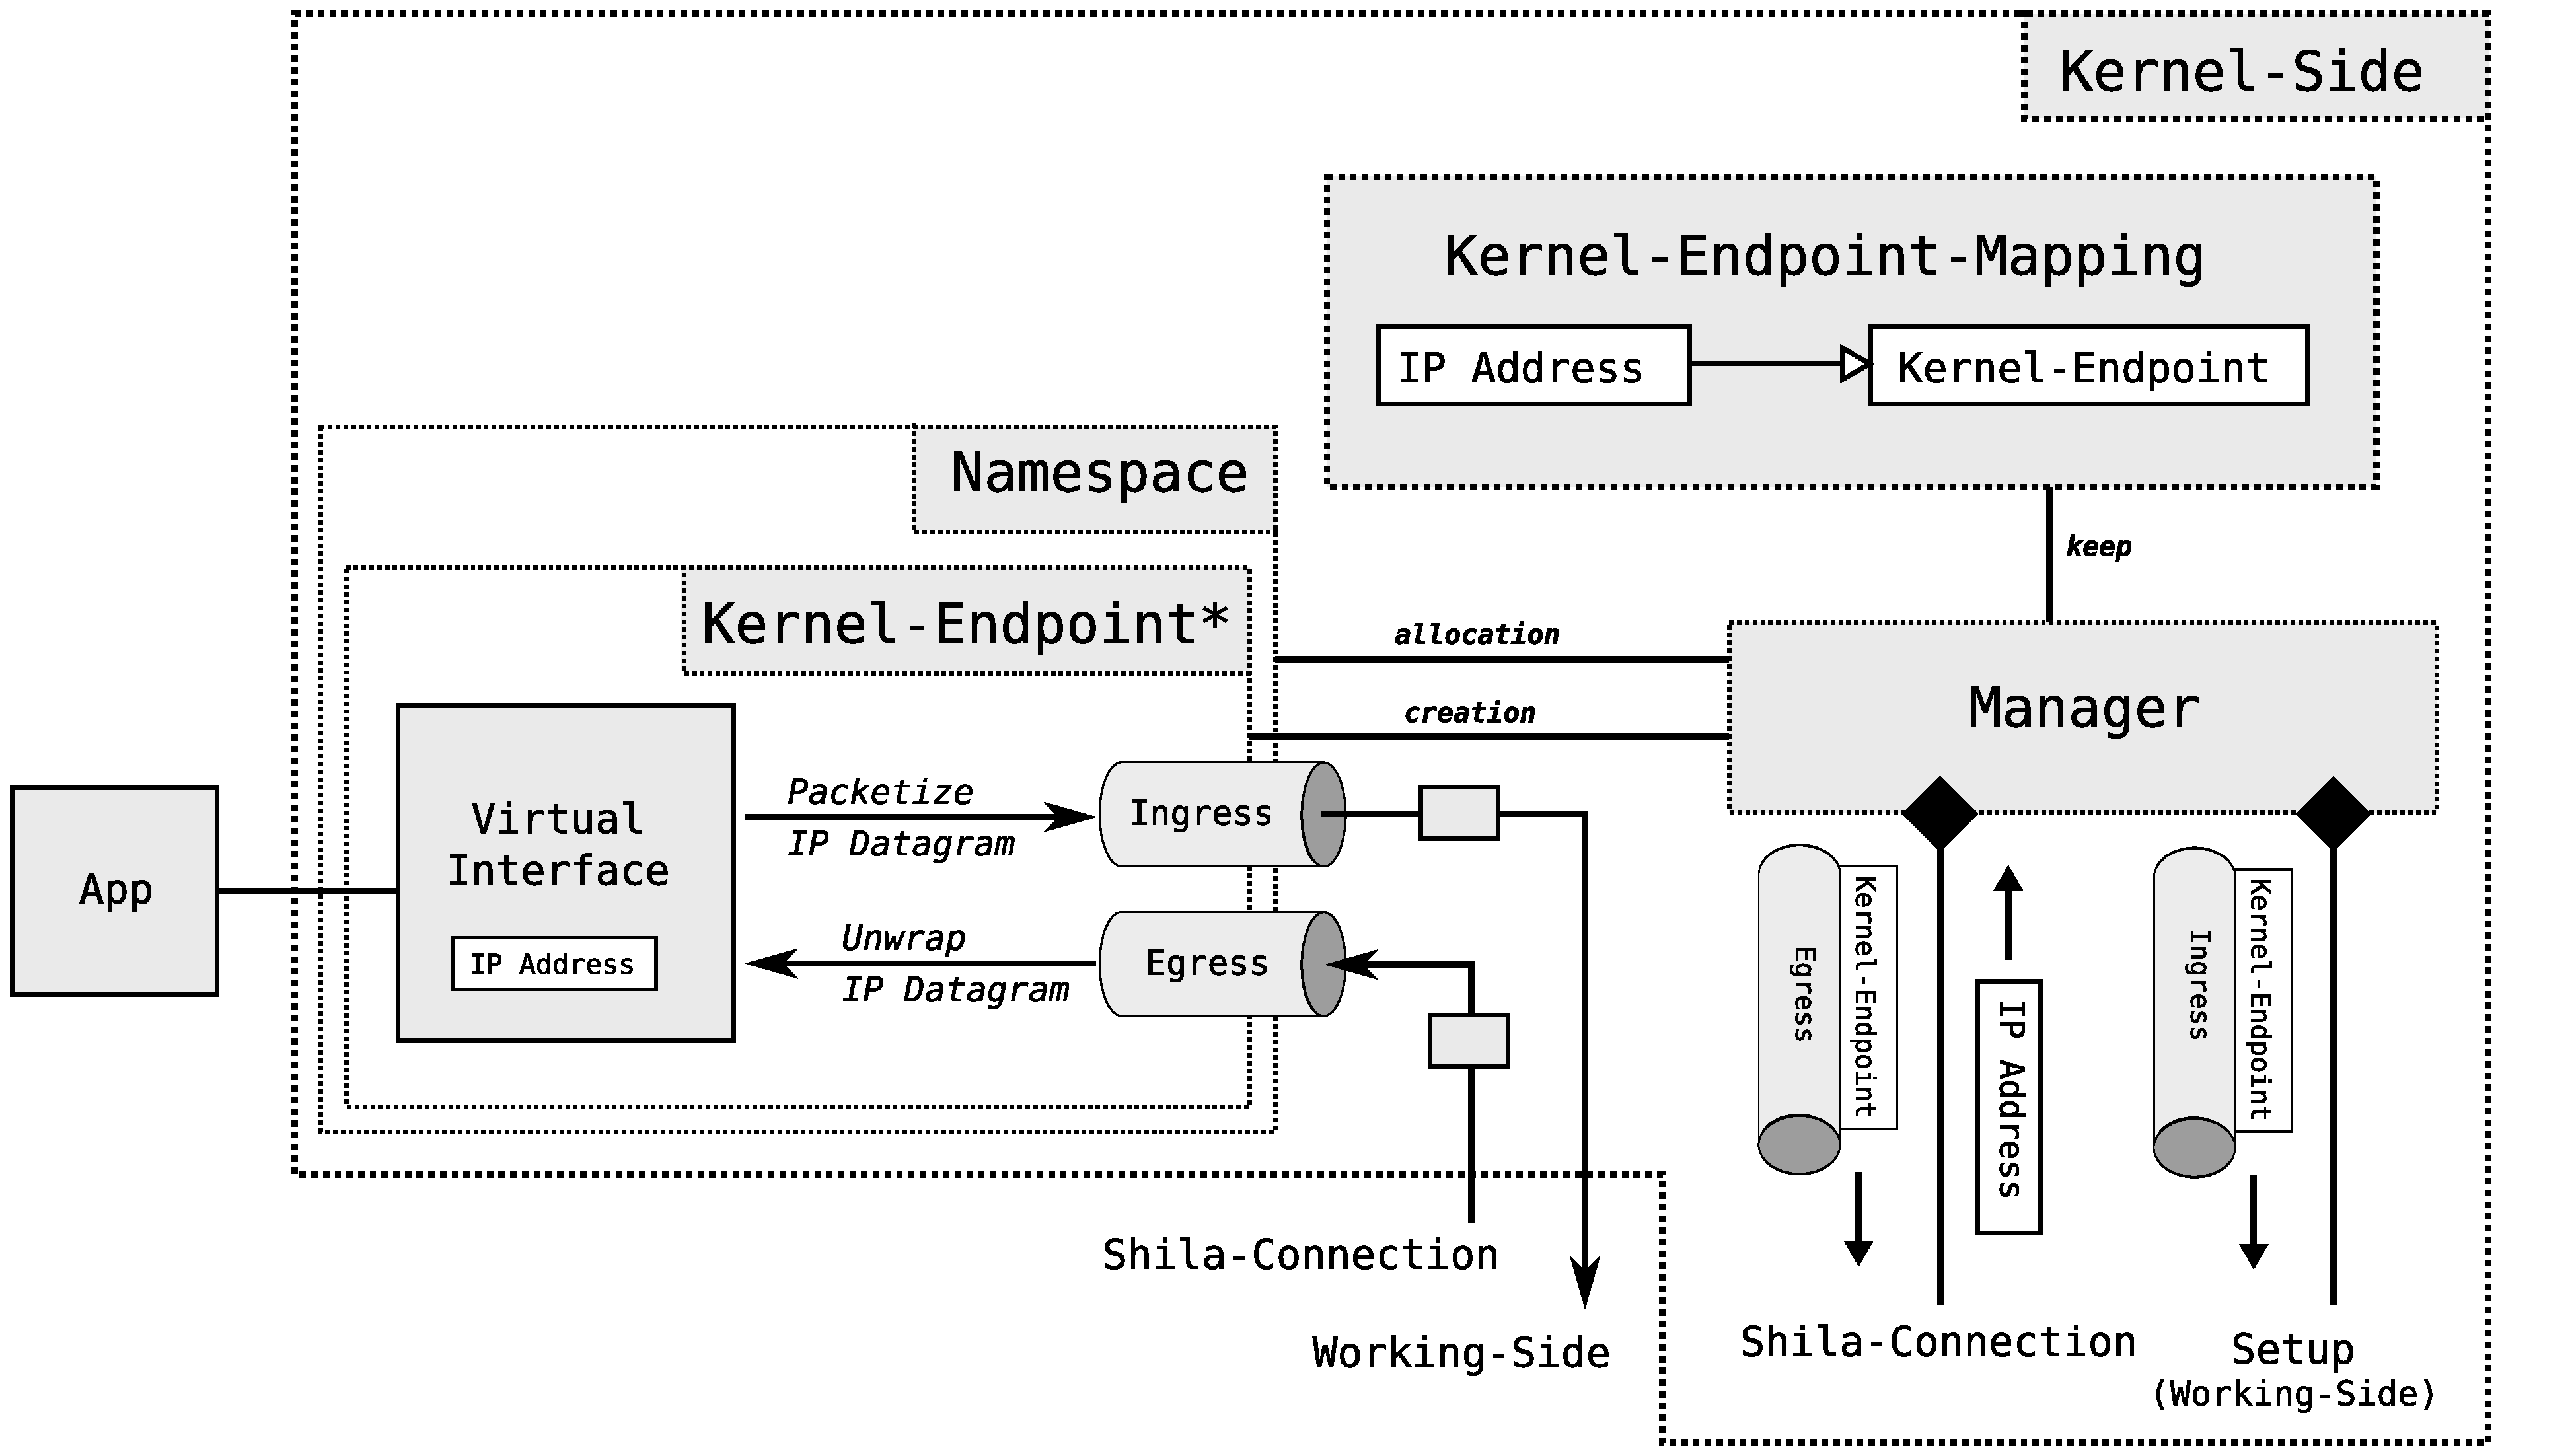
\includegraphics[scale=0.2]{../illustrations/implementation/ModulesKernelSide.pdf}   
		\caption[Caption for the list of figures.]{Illustration of the Kernel-Side with its subparts.}
		\label{fig:ImplementationModulesKernelSide}
	\end{center}
\end{figure}


\subsubsection{Kernel-Endpoint}

The Kernel-Endpoint creates and holds the virtual network interface over which the data exchange with the TCP endpoints takes place. Every Kernel-Endpoint is identified by an IP address, namely the IP address assigned to its underlying virtual interface. It also holds two traffic channels. For an IP frame received through the virtual interface, the TCP-Flow is determined and a newly created Shila-Packet is sent via the ingress channel to the working side. Through the egress channel packets from Shila-Connections are received. From these packets, the payload is taken and transferred to the virtual interface and from there to the TCP endpoint.

\subsubsection{Virtual Interface}

Shila uses the Universal TUN/TAP device driver \cite{TUNTAPDriver} to set up virtual network devices on the host. Such a virtual network device is perceived by the kernel as a real Ethernet device. The difference is that traffic from the kernel is not sent through a physical medium but can be read by an application, in our case Shila. On the other hand, the virtual device does not receive the data over the cable but from an application, again Shila.

Each virtual network interface has an IP address assigned to it. When a TCP endpoint sends data over a virtual device, Shila receives the corresponding IP datagrams. Each of these contains a TCP flow. The source TCP address consists of the IP address of the virtual device and an arbitrary port. The destination address is the TCP address the application wants to send data to. Conversely; when Shila writes payload, an IP datagram, to a virtual device, then the kernel forwards it to the application identified by the destination TCP address.  

\subsection{Network-Side}

The Network-Side is also orchestrated by an appropriate manager. At startup, the manager takes care of establishing the Contact-Server-Endpoint. It furthermore provides the interface to Shila-Connections for the creation of new Contact-Client-Endpoints, Traffic-Client-Endpoints and Traffic-Server-Endpoints. The Network-Side holds three different mappings. Two to get the corresponding Client-Endpoint for a given TCP-Flow, and one to get the Server-Endpoint associated with the SCION source address. These mappings are only used by the manager to interact with the endpoints, e.g. for the deallocation in case of a disconnection. They are not needed for the data exchange itself. After establishing the connection, the corresponding entities directly hold a handle of the traffic channels from the respective endpoints. Figure \ref{fig:ImplementationModulesNetworkSide} illustrates these Network-Endpoint-Mappings as part of the whole kernel side and its subparts.  

\subsubsection{Server-Endpoint}

The Server-Endpoint is one of two types of Shila-Endpoints found on the Network-Side. It can be further divided into Contact-Server-Endpoint and Traffic-Server-Endpoint. However, there is no difference in basic functionality between the two. We mention the differences in the discussion of setup¨ and connection establishment, see Section \ref{sec:ImplementationSetup} and Section \ref{sec:ImplementationConnectionEstablishment}.

A Server-Endpoint holds and handles a collection of Backbone-Connections, i.e. connections through the SCION network to Client-Endpoints running on other instances of Shila. Each such Backbone-Connection is associated with a Net-Flow. The Server-Endpoint-Mapping\footnote{In Figure \ref{fig:ImplementationModulesNetworkSide}, this mapping is shown as part of the Network-Endpoint-Mappings.} in the Network-Side uses the source address of this Net-Flow as a key. Inside the endpoint, the corresponding destination address is used as the key for the Backbone-Connection-Mapping. %Note that this mapping is used in the actual data exchange. 

A Backbone-Connection itself uses the appnet package \cite{Appnet} to establish the connection in SCION. Data received from the SCION network is packed into a Shila packet by the responsible backbone connection and sent via the ingress traffic channel of the server to the Working-Side. Packets received from Shila-Connections are allocated to their Backbone-Connection using their Net-Flow and the Backbone-Connection-Mapping. From there, the payload is sent to the SCION network.

\subsubsection{Client-Endpoint}

The Client-Endpoint is the other type of Shila-Endpoints within the Network-Side. It is the initiating party of a Backbone-Connection and is associated with just a single Net-Flow. As with the Server-Endpoint, a distinction is made between a Contact-Client-Endpoint and a Traffic-Client-Endpoint, again discussed later. The data exchange between the SCION network and the internal Shila units works via the appnet package and two traffic channels. Since only one Backbone-Connection is assigned to a single Client-Endpoint, no mapping is required inside the endpoint.

\begin{figure}
	\begin{center}
		\def\svgwidth{1\textwidth}
		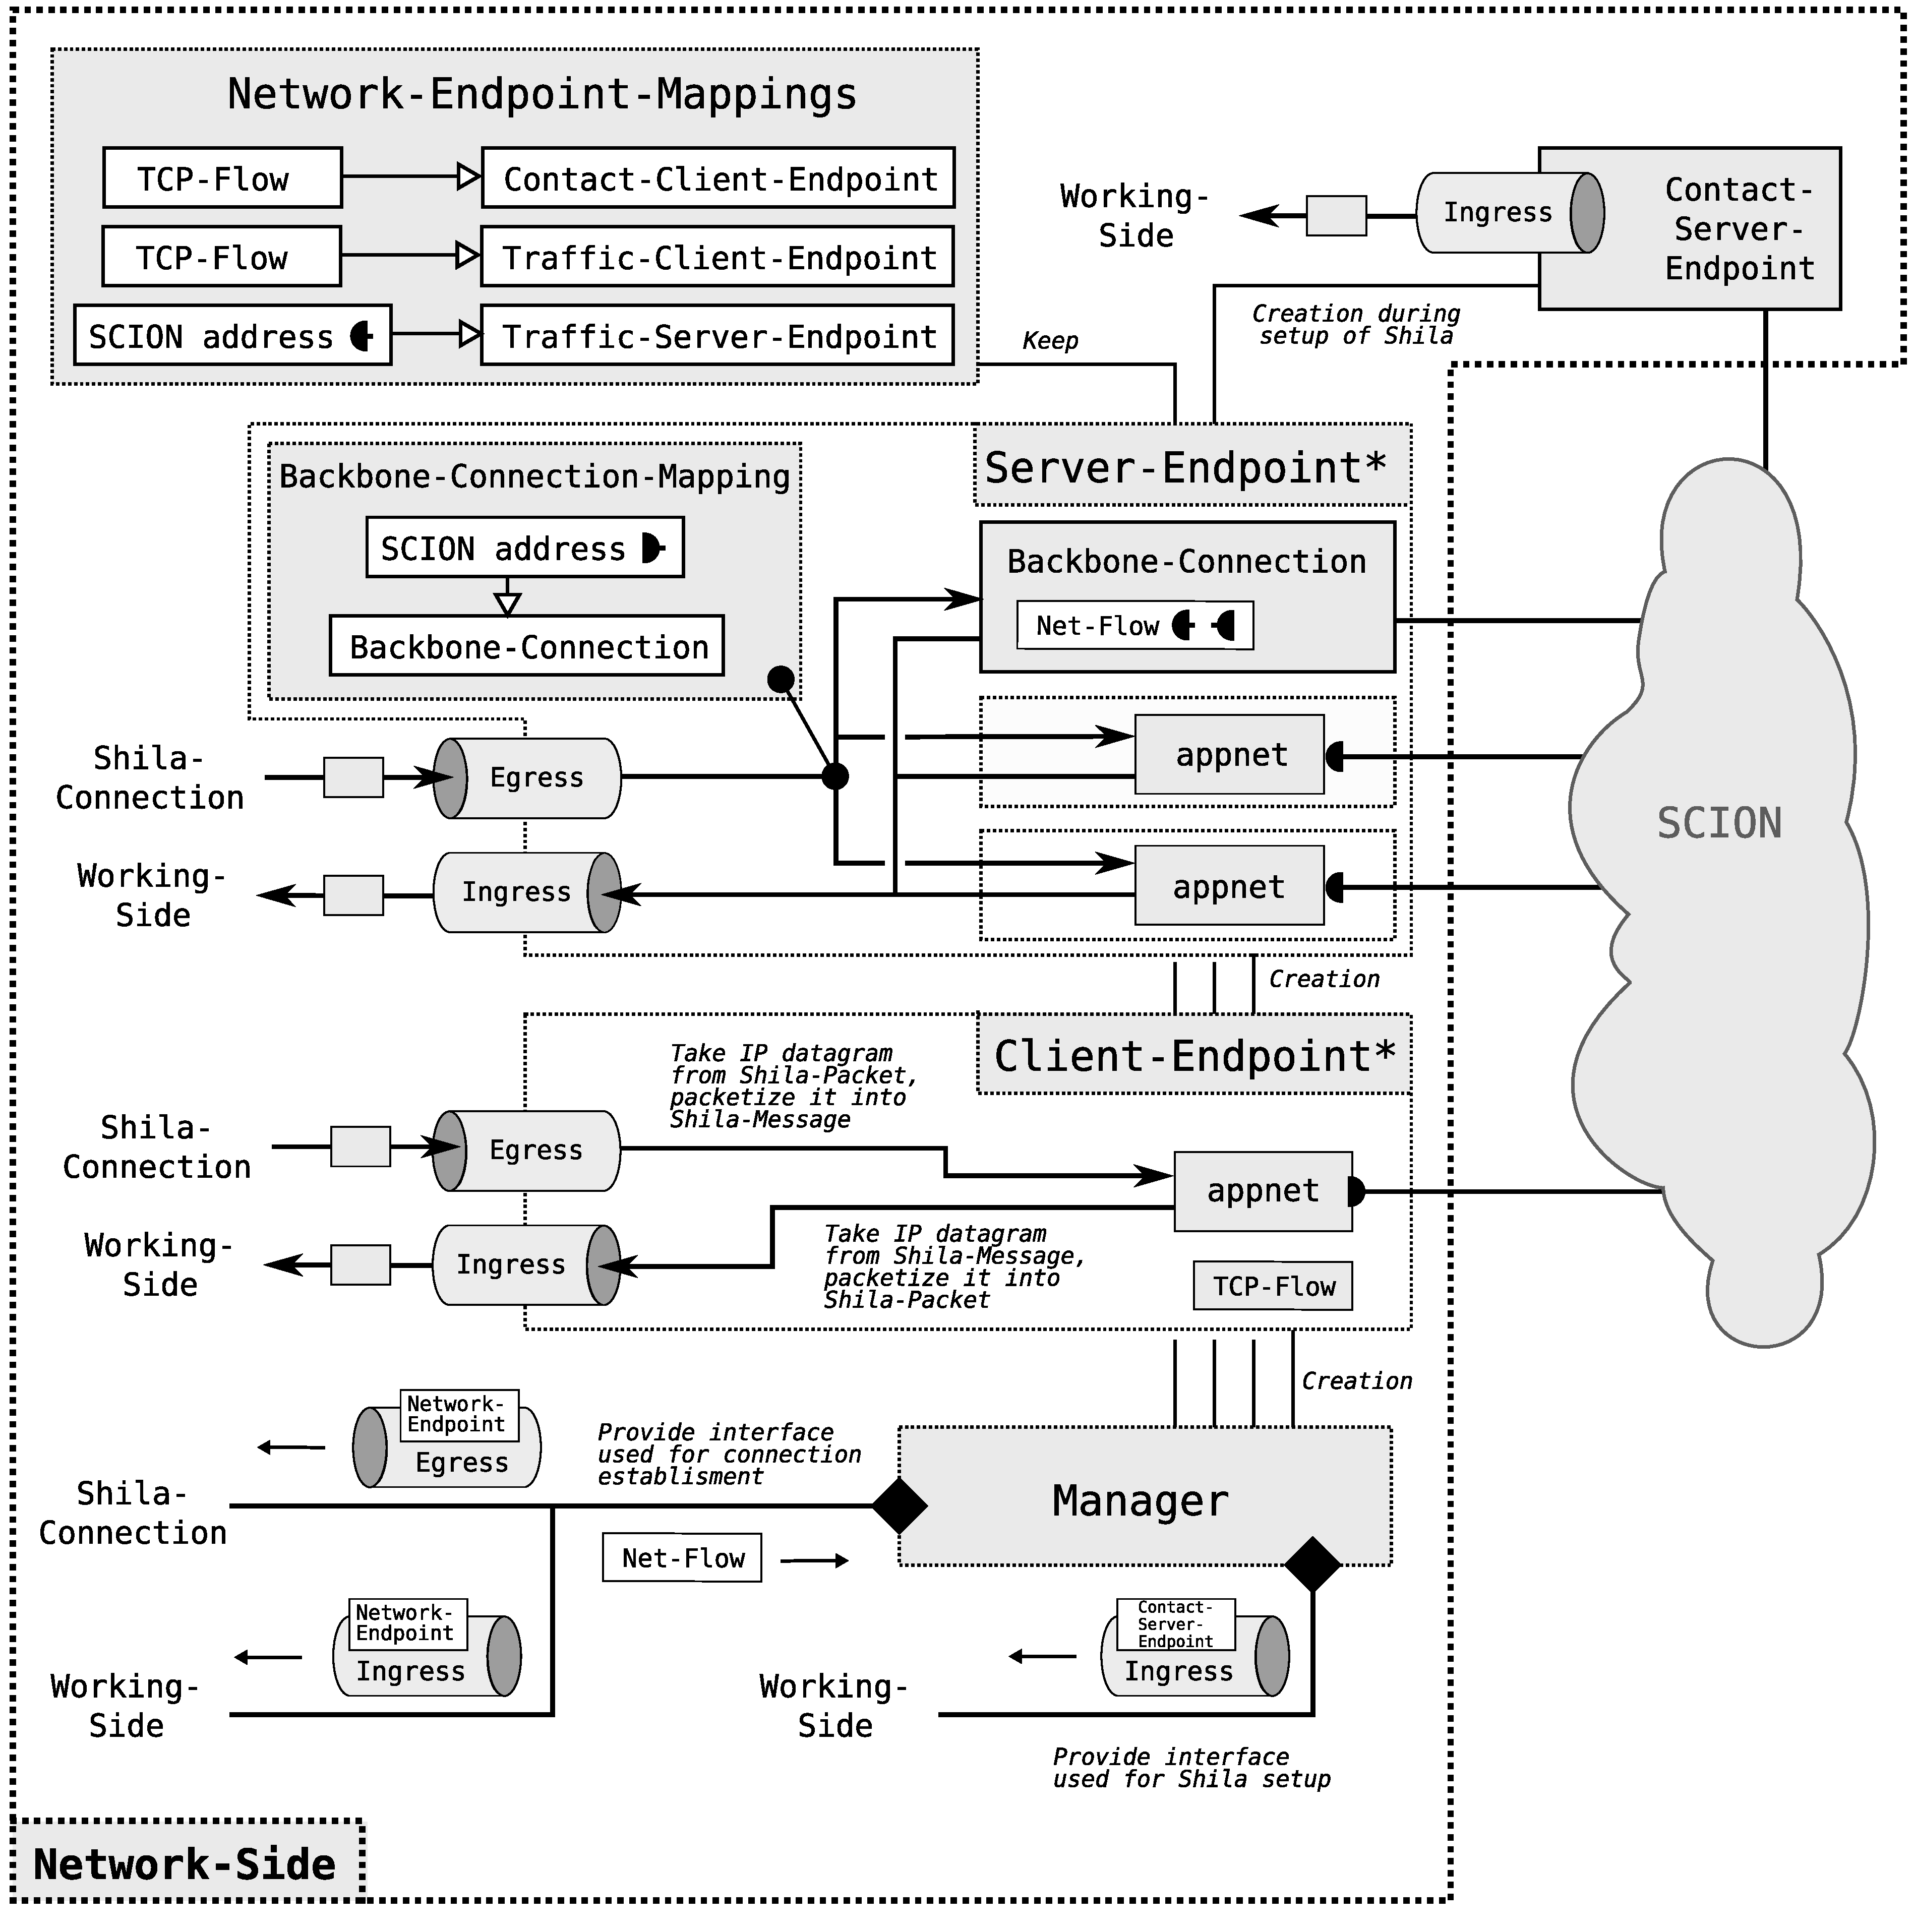
\includegraphics[scale=0.2]{../illustrations/implementation/ModulesNetworkSide.pdf}   
		\caption[Caption for the list of figures.]{Illustration of the Network-Side with its subparts.}
		\label{fig:ImplementationModulesNetworkSide}
	\end{center}
\end{figure}

\subsection{Working-Side}

Upon the arrival of a Shila-Packet at the Working-Side it is processed by a dedicated worker. Its TCP-Flow is extracted and used as the key for the Shila-Connection-Mapping, the heart of the Working-Side. It contains the mapping from TCP-Flows to Shila-Connections. If there is no corresponding entry available then a new Shila-Connection is created and inserted into the mapping. Once obtained, the responsible worker processes the Shila-Packet through the associated Shila-Connection. The described process is illustrated in Figure \ref{fig:ImplementationProcessWorkingSide}.

\begin{figure}[H]
	\begin{center}
		\def\svgwidth{1\textwidth}
		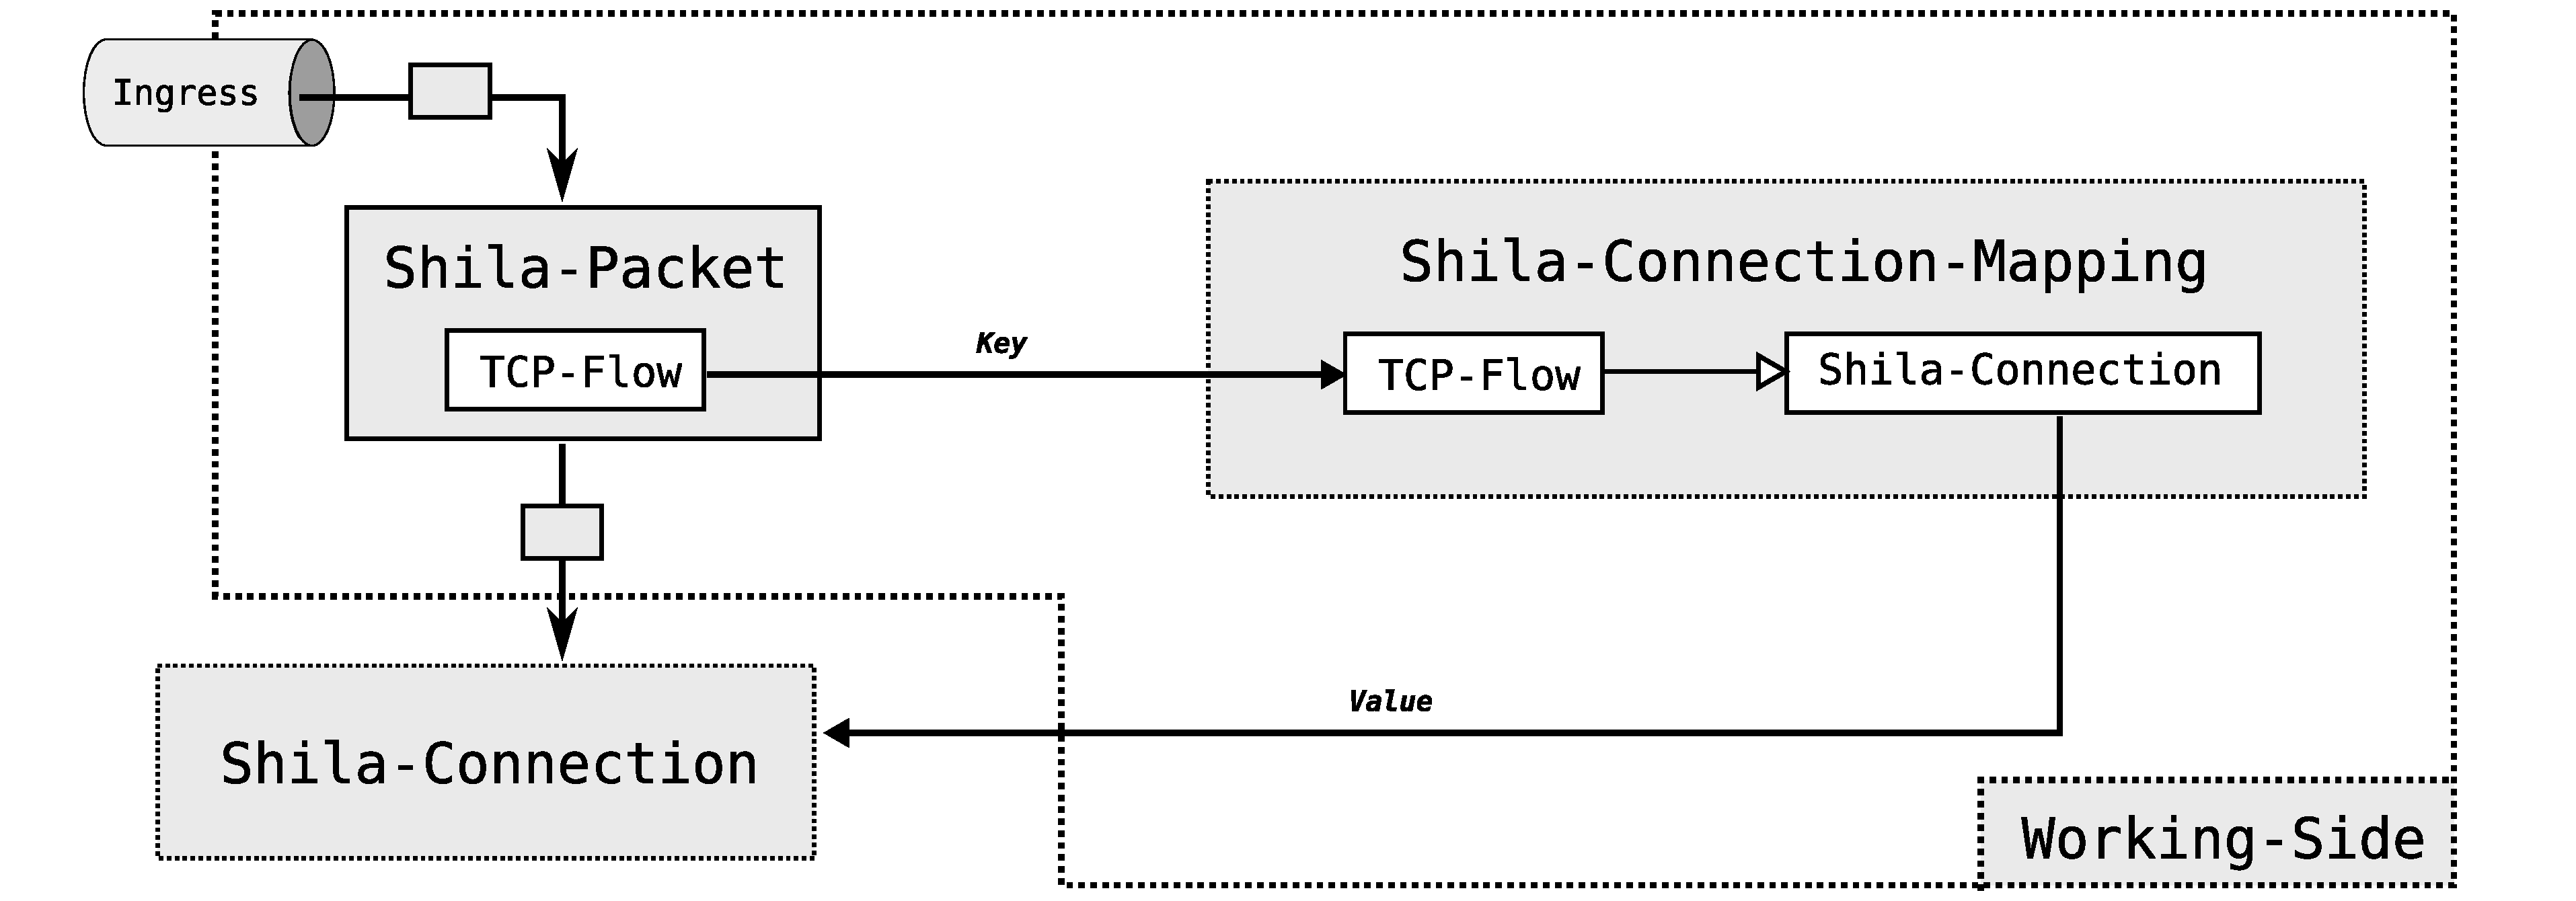
\includegraphics[scale=0.2]{../illustrations/implementation/ProcessWorkingSide.pdf}   
		\caption[Caption for the list of figures.]{Illustration of the Working-Side.}
		\label{fig:ImplementationProcessWorkingSide}
	\end{center}
\end{figure}

\subsection{Shila-Connection}

The Shila-Connection, depicted in Figure \ref{fig:ImplementationShilaConnection}, is the main part of Shila, with its logic responsible for establishing and maintaining connections. The centerpiece is the state machine and the close coupling to the router, which provides SCION destination and path information. During connection establishment, the Shila-Connection uses the interfaces of Kernel-Side and Network-Side as well as the functionalities provided by the Router to put its traffic channels into place. Once established, the packages flow smoothly through the Shila-Connection to their respective destination endpoints without much interaction. Every Shila-Connection is identified by its TCP-Flow and holds, once the connection is established, the corresponding Net-Flow.

\begin{figure}
	\begin{center}
		\def\svgwidth{1\textwidth}
		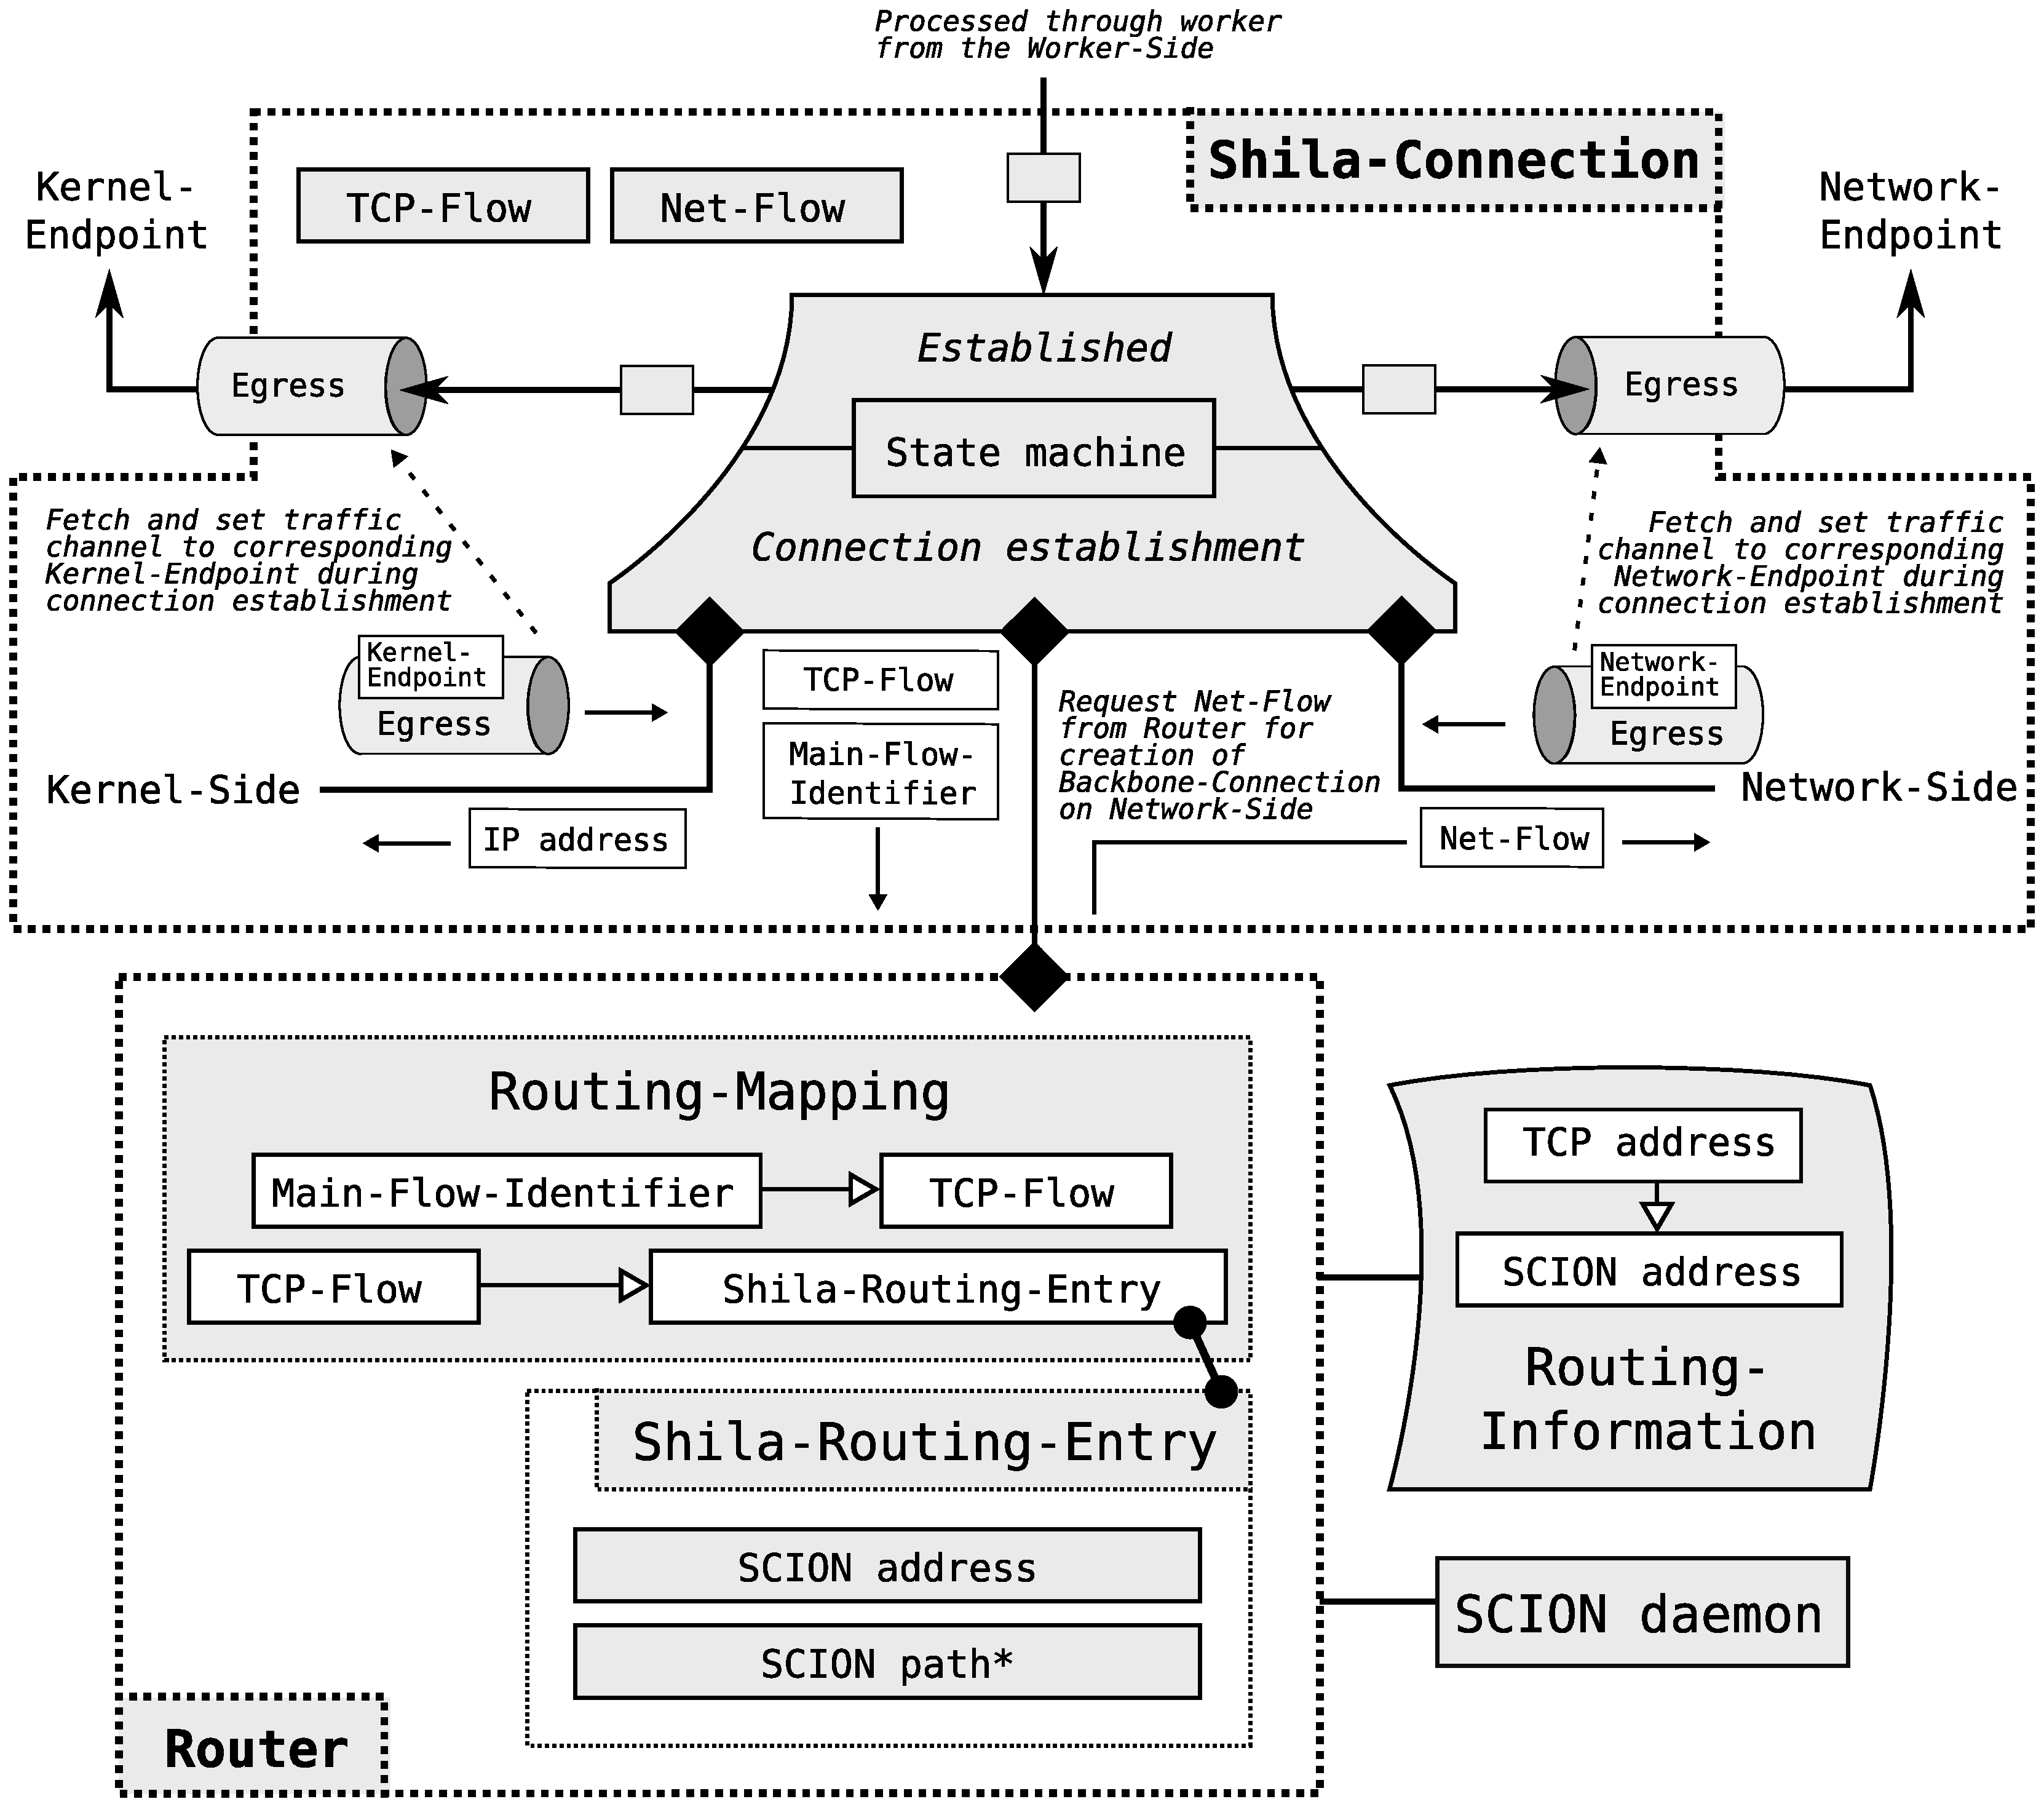
\includegraphics[scale=0.2]{../illustrations/implementation/PartsShilaConnection.pdf}   
		\caption[Caption for the list of figures.]{Illustration of the Shila-Connection together with the Router. The Shila-Connection receives the packets assigned to it through the Working-Side. If the connection is already established, the packet is forwarded directly to its destination via the egress traffic channel. During the connection setup, the Shila-Connection first uses the Router to determine the Net-Flow and then requests the egress traffic channels from the Kernel-Side and Network-Side.}
		\label{fig:ImplementationShilaConnection}
	\end{center}
\end{figure}

\subsection{Router}
\label{sec:ImplementationRouter}

The Router supplies the Shila-Connection with the Net-Flow as part of the connection establishment. It is connected to the SCION daemon running on the host and has access to a hardcoded mapping between TCP and SCION addresses. This mapping is denoted as Routing-Information. The Router illustrated as part of Figure \ref{fig:ImplementationShilaConnection} also maintains a Routing-Mapping which uses TCP-Flow as a key to store Shila-Routing-Entries and an additional mapping from Main-Flow-Identifier to TCP-Flows.

\subsubsection{Shila-Routing-Entry}

A Shila-Routing-Entry stores a SCION address and several paths leading through the SCION network to this destination. The number of stored paths depends on the setting of Shila, namely on the number of virtual interfaces created in the egress namespace. Also stored for each of the paths is its quality, given in different metrics. These metrics are used as a decision criterion in the process of path selection which is itself part of the creation of routing entries. The whole process of the routing, i.e. the creation of these entries as well as the procedure of path selection is described in its own Section \ref{sec:ImplementationPathSelection}.

\newpage
\section{Setup}
\label{sec:ImplementationSetup}

In this section, we describe the crucial steps executed during the setup of Shila. The description is similar to the one given in the Introduction to Shila, Subsection \ref{subsec:ShilaSetup}. This time its more detailed and also refers to the structure presented in the sections and illustrations above.

\paragraph{Loading of the Routing-Information}

To perform its function of providing translations between a TCP-Flow and a Net-Flow, the Router establishes a connection to the SCION daemon and loads the Routing-Information from disk. Saved as a JSON file it contains the translation from a TCP to a SCION address. Currently, there is no other way to provide the Router with this necessary information. However, alternatives are certainly conceivable and are mentioned in the concluding Chapter \ref{chap:FutureWork}.

\paragraph{Setup of Namespaces}

The manager on the kernel side creates the two network namespaces \cite{LinuxNetworkNamespacesUbuntuManual,LinuxNetworkNamespacesIntroduction}, the ingress and the egress namespace, in a first step. System resources, like network devices or IP routing tables, associated with networking and assigned to different namespaces are isolated from each other. This simplifies the development and setup of the kernel side but on the downside requires the TCP applications to be started within the corresponding namespaces. For further discussions with regard to namespaces see Chapter \ref{chap:FutureWork}.

\paragraph{Creation of Kernel-Endpoints hosting virtual Interfaces}

In the second step, the manager creates the Kernel-Endpoints in the appropriate namespaces. In the ingress namespace, this is exactly one, in the egress namespace, this is a number selected by the user between one and a maximum of eight. The number of Kernel-Endpoints selected in the egress namespace later corresponds to the number of paths used for a connection. The current implementation of MPTCP supports up to eight interfaces. Having Shila to support more is therefore useless, but can be realized without problems if necessary in the future.

Each Kernel-Endpoint contains a virtual interface to which an IP address is assigned. This address is also assigned to the Kernel-Endpoint itself and is used as a key in the Kernel-Endpoint-Mapping. The virtual interface in the ingress namespace is assigned a default address (10.7.0.9), the assignment in the egress namespace is done at random. Upon its establishment, every Kernel-Endpoint creates two traffic channels. The ingress channel, which is used for forwarding incoming data, is registered at the working side. 

\paragraph{Contact-Server-Endpoint}

During the setup, the manager in the Network-Site creates just one Network-Endpoint; the Contact-Server-Endpoint. This endpoint starts listening for incoming Backbone-Connections on the default SCION port 7654 using the appnet package. In contrast to all other Shila-Endpoints, it needs only one traffic channel, namely for incoming messages that initiate the establishment of a new connection. This channel is registered with the Working-Side.

After the successful setup, applications can be started in the respective namespaces and the data exchange is initiated with the connection establishment.

\section{Connection Establishment}
\label{sec:ImplementationConnectionEstablishment}

In this section, we again discuss the individual steps in the establishment of a new connection between two TCP endpoints. We use the explanation of Section \ref{subsec:ShilaConnectionEstablishment} as a basis, but go into more detail and extend the sequence with intermediate steps, referring to the treatise of the structure given in Section \ref{sec:ImplementationStructure}. The starting point and the example used is the same one as used in the introductory treatise of the connection establishment in Section \ref{subsec:ShilaConnectionEstablishment}. Illustration \ref{fig:ConnectionEstablishment} shows the state after the successful establishment of the connection with the values from the example discussed. These values are also mentioned in the discussion of the individual steps below. In the used notation, the source comes first and then the destination.

\subsection{Main-Flow Establishment}

We start with a more detailed discussion of the Main-Flow establishment. 

\begin{description}
	\item[M-1] On Host 2, the server instance of iPerf3 starts listening for incoming TCP connections. It, therefore, binds to the virtual interface in the Shila ingress namespace on the TCP address 10.7.0.9:27041. This step is not recognized by the Kernel-Endpoint hosting the corresponding virtual interface.
	\item[M-2] On Host 1, the client instance of iPerf3 tries to connect to its server counterpart on TCP address 10.7.0.9:27041. For the connection establishment, an IP datagram, containing the TCP-SYN, is sent via one of the virtual interfaces in the egress namespace. Let's say It is identified by the IP address 10.0.0.1 and the socket bound to port 11111.
	\item[M-3] The Kernel-Endpoint owning the corresponding virtual interface receives the IP datagram and puts it into a Shila-Packet. While payload, Shila-Endpoint and TCP-Flow$^{1}$ are determined, the Net-Flow for the created Shila-Packet is not yet known. The packet is now forwarded to the Working-Side.\medskip\\{\small[10.0.0.1:11111, 10.7.0.9:27041]$^{1}$}
	\item[M-4] The Working-Side uses the TCP-Flow, extracted from the packet, as the key into the Shila-Connection-Mapping. Since there is no corresponding Shila-Connection, a new one is created and the Shila-Packet is forwarded on to it.  
	\item[M-5] To be able to forward the received Shila-Packet, the newly created Shila-Connection has to first determine the destination SCION address and path. It does this by querying the Router, which determines the corresponding parts of the Net-Flow for the TCP-Flow of the packet.
\end{description}

The entire process of determining the Net-Flow, i.e. address translation and the path selection, is explained in the following Section \ref{sec:ImplementationPathSelection}. To include the explanation as part of this sequence, would make it unnecessary bulky to read. For the next step M-6, we assume that the required parts of the Net-Flow are determined.

\begin{description}
	\item[M-6] The Shila-Connection uses the interface of the manager on the Network-Side to initiate the creation of a Contact-Client-Endpoint. It provides the Net-Flow$^2$ it has received from the Router.\medskip\\{\small[1-ff00:0:112,127.0.0.1, 2-ff00:0:220,127.0.0.1:27041]$^2$}
	\item[M-7] The Contact-Client-Endpoint establishes the so-called Contact-Backbone-Connection to the Contact-Server-Endpoint. It uses the source address available in the provided Net-Flow together with the default SCION port of the listening server. For our example, we assume that the outgoing SCION port of the Contact-Client-Endpoint is 12121. This information completes the Net-Flow of the Contact-Backbone-Connection$^{3}$.\medskip\\{\small [1-ff00:0:112,127.0.0.1:12121, 2-ff00:0:220,127.0.0.1:7654]$^{3}$}
%\end{description}
%	
%The establishment of a Backbone-Connection between Client-Endpoint and Server-Endpoint is described separately in Section %\ref{sec:ImplementationEstOfBackboneConnections}. For the next step, \textbf{M-9}, we assume that the Backbone-Connection %between Contact-Client-Endpoint on Host 1 and Contact-Server-Endpoint on Host 2 is established.
%	
%\begin{description}
	\item[M-8] With the successful setup of the Contact-Client-Endpoint, the Shila-Connection receives the handle to its egress traffic channel. Using this channel, the Shila-Packet, and hence the initial IP datagram containing the TCP-SYN is now transferred to the Contact-Server-Endpoint running on the Shila instance on Host 2. %The Shila-Connection sets its Net-Flow$^{3}$ to be the one of the Contact-Backbone-Connection.%
	\item[M-9] The IP datagram is received at the Contact-Server-Endpoint on Host 2. There, it is put into a Shila-Packet and forwarded via the ingress traffic channel to the working side. The Net-Flow$^{4}$ (namely that of the backbone connection between Contact-Client-Endpoint and Contact-Server-Endpoint) can already be assigned to the newly created Shila-Packet. The TCP-Flow$^{5}$ is also known since it was transmitted with the establishment of the Contact-Backbone-Connection.\medskip\\{\small [2-ff00:0:220,127.0.0.1:7654, 1-ff00:0:112,127.0.0.1:12121]$^{4}$}\\{\small [10.7.0.9:27041, 10.0.0.1:11111]$^{5}$} 
	\item[M-10] The Working-Site on Host 2 cannot find a Shila-Connection for the TCP-Flow$^{5}$ in the Shila-Packet. Accordingly, a new one is created and the packet is passed to it.
	\item[M-11] Inside the Shila-Connection, three tasks are performed. First, the Net-Flow$^{4}$ of the Shila-Packet is extracted and assigned to the Shila-Connection.  Note, until now it was the Net-Flow of the associated Contact-Backbone-Connection. Second, the Shila-Packet is forwarded. The source IP address of its TCP-Flow$^{5}$ is used to retrieve the egress traffic channel from the Kernel-Endpoint residing in the ingress namespace. This is done by the Shila-Connection by querying the Kernel-Endpoint-Mapping inside the Kernel-Side. For our example, the IP address used as the key is 10.7.0.9. The Shila-Packet is forwarded through the respective channel, once it is obtained. Third, the Shila-Connection causes the creation of a Traffic-Server-Endpoint which is ready for new Backbone-Connections at SCION port 27041. The ingress traffic channel is registered with the Working-Side and the Shila connection receives a handle to respective the egress traffic channel.
	\item[M-12] The Kernel-Endpoint receives the Shila-Packet, extracts its payload and sends the IP datagram containing the TCP-SYN through the virtual interface towards the listening iPerf3 server instance.
	\item[M-13] In the meantime, the Shila connection of Host 1 has initiated the creation of a Traffic-Client-Endpoint. This now establishes a Backbone-Connection to its opposite, called a Traffic-Backbone-Connection. This time, in comparison to step M-8, using the complete Net-Flow. Let's assume that the Traffic-Client-Endpoint binds locally to SCION port 34343, completing the Net-Flow$^{6}$ of the Traffic-Backbone-Connection. This Net-Flow is assigned to Shila-Connection on Host 1.
	\medskip\\{\small [1-ff00:0:112,127.0.0.1:34343, 2-ff00:0:220,127.0.0.1:27041]$^{6}$}
	\item[M-14] With the successful establishment of the Traffic-Backbone-Connection, the involved Server-Endpoint on Host 2 receives the TCP-Flow$^{5}$ as well as two Net-Flows. The Net-Flow$^{4}$ of Contact-Backbone-Connection and the Net-Flow$^{7}$ of the Traffic-Backbone-Connection. Both of its destination addresses are used as key to store the Traffic-Backbone-Connection in Backbone-Connection-Mapping. This is required since the Shila-Connection sends back all data, including the data received via the Contact-Server-Endpoint, via the Traffic-Server-Endpoint. Remember, the Shila-Connection on Host 2 currently holds the Net-Flow of the Contact-Backbone-Connection which now can be updated to the one of the Traffic-Backbone-Connection.\medskip\\{\small [2-ff00:0:220,127.0.0.1:27041, 1-ff00:0:112,127.0.0.1:34343]$^{7}$}
\end{description}	
	\begin{landscape}
		\begin{figure}
			\begin{center}
				\def\svgwidth{1\textwidth}
				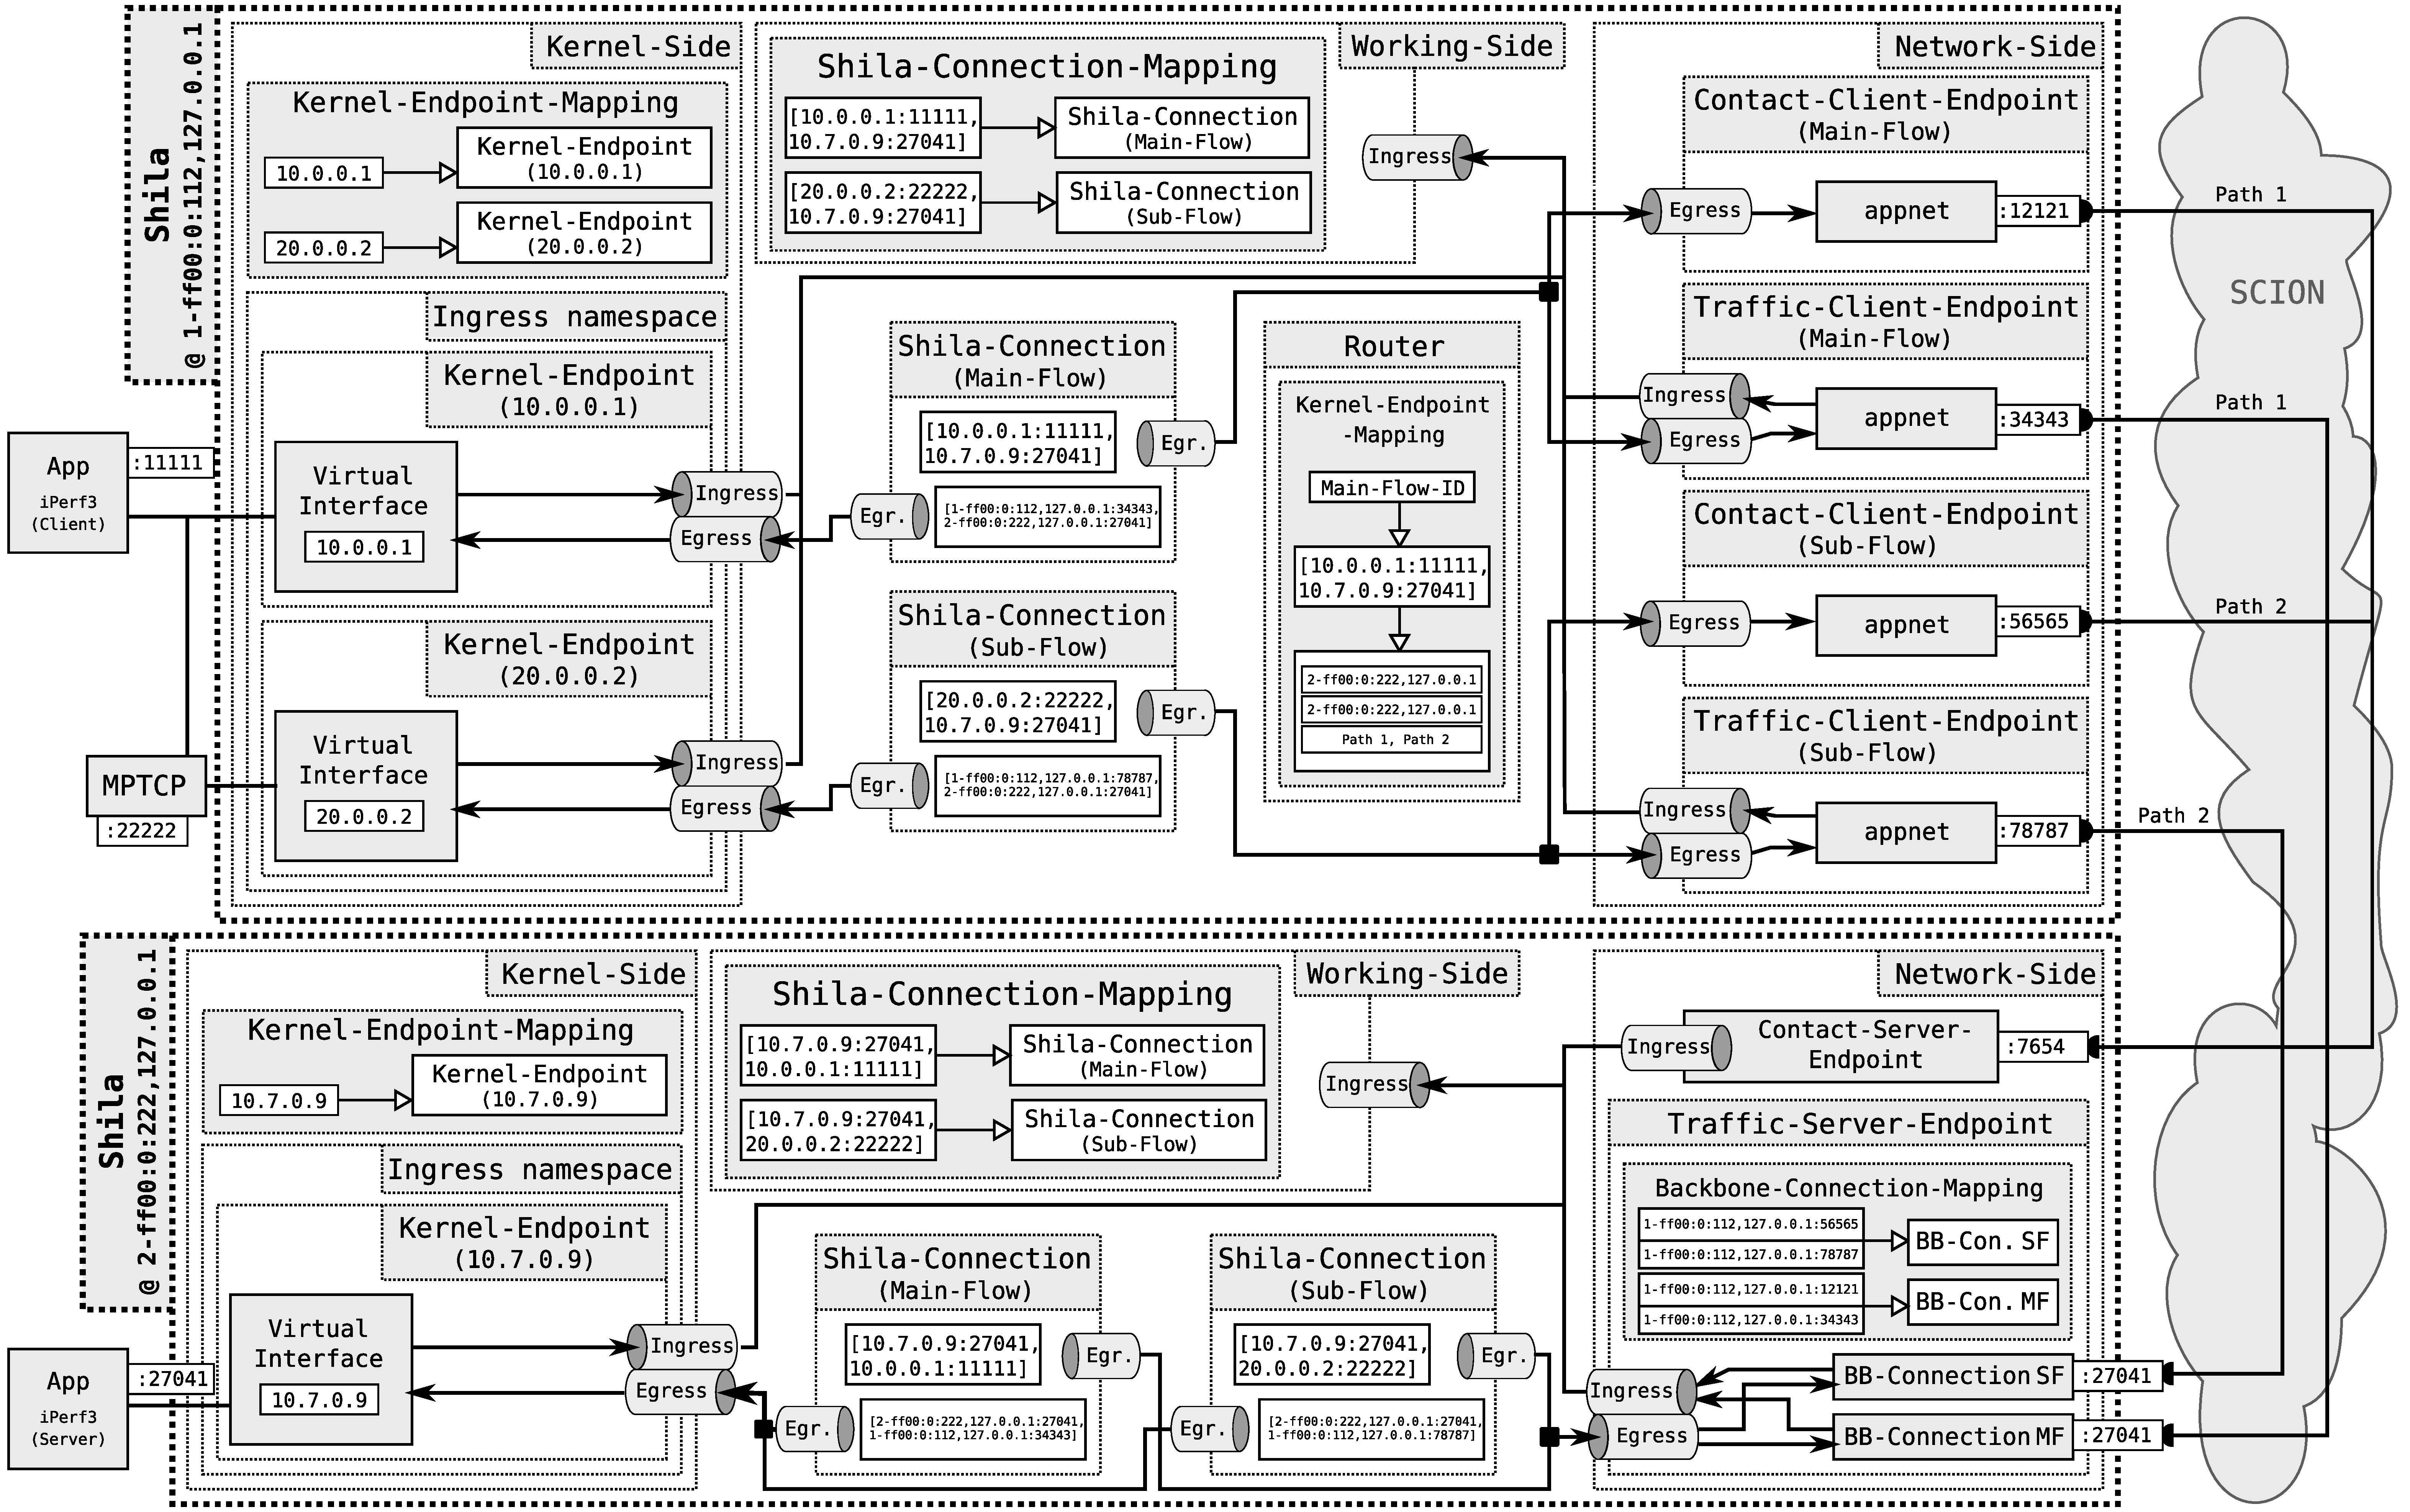
\includegraphics[scale=0.2]{../illustrations/implementation/ConnectionEstablishment.pdf}   
				\caption[Caption for the list of figures.]{Illustration of the State of the Shila instances after the establishment of the Main-Flow and one Sub-Flow. Note that the Contact-Backbone-Connections are removed as soon as the establishment was successful. We show them just for demonstrative purpose.}
				\label{fig:ConnectionEstablishment}
			\end{center}
		\end{figure}
	\end{landscape}
\begin{description}		
	\item[M-15] The IP datagram containing the answer from the iPerf3 server instance, a TCP-SYN+ACK, arrives at the Kernel-Endpoint at Host 2. From there the answer travels in a Shila-Packet, using its TCP-Flow$^{5}$, through the Working-Site to the corresponding Shila-Connection.
	\item[M-16] The Shila-Connection assigns its Net-Flow to the Shila-Packet and forwards it via traffic channel to the corresponding Traffic-Server-Endpoint. From there the TCP-SYN+ACK data finds its way through the Traffic-Backbone-Connection to the corresponding client part. 
	\item[M-17] The reception of the first data from the Traffic-Client-Endpoint on Host 1 concludes the connection establishment. The first response from the Iperf3 Server instance reaches the Shila-Connection, where the Main-Flow-Identifier is extracted. This identifier is used to update the Router accordingly such that Sub-Flows created later can be assigned to their Main-Flow. The response, holding the TCP-SYN+ACK, is then sent along the traffic channel toward the client instance of iPerf3.
	\item[M-18] The Contact-Backbone-Connection is no longer needed and can therefore be removed, together with its corresponding Network-Endpoints.
\end{description}

As soon as the Main-Flow is established, MPTCP starts to initiate further flows, triggering the establishment of Sub-Flows over the other virtual interfaces.

\subsection{Sub-Flow Establishment}

The establishment of Sub-Flow works in the same way as that of a Main-Flow. Therefore, in the following, only the deviating points are mentioned. Of course, the individual entities bind to other ports. But this is not explicitly mentioned and should be clear in illustration \ref{fig:ConnectionEstablishment}.

\begin{description}	
\item[S-2] The initiation for the Sub-Flow is made by MPTCP itself. It binds to one of the yet unused virtual interfaces on Host 1. For our example we assume that port 22222 is chosen. 
\item[S-5] The Router already has an entry, holding destination address and paths. For the establishment of the Sub-Flow, It is sufficient for the Shila-Connection to submit the Main-Flow-Identifier to get the required Net-Flow.
\end{description}

\newpage
\section{Path Selection}
\label{sec:ImplementationPathSelection}

In this section, we discuss the process of determining the Net-Flow given a TCP-Flow or Main-Flow-Identifier. It takes place in the Router and is illustrated as part of Figure \ref{fig:ImplementationShilaConnection}.

During the connection establishment, the Router gets a request from the involved Shila-Connection. It provides either a TCP-Flow if a Main-Flow is about to be established or a Main-Flow-Identifier if a Sub-Flow is about to be established. We start with the explanation of the former and then deal with the latter.

\subsection*{Path Selection in the Main-Flow Establishment}

The Shila-Connection is requesting the Net-Flow for a given TCP-Flow. That is, the Router has to determine and handle the three different entries.

\begin{description}
	\item[Source address] This is the address of the host running the current Shila instance and can be requested from the SCION daemon.
	\item[Destination address] The Router first extracts the destination TCP address from the TCP-Flow. Then a request, using the extracted address as key, is placed into the Routing-Information to fetch the corresponding SCION destination address.
	\item[Path] By querying the SCION daemon the Router receives a set of possible paths leading to the previously fetched destination address. From this collection, the Router selects the best possible subset and stores it together with the SCION destination address in a Shila-Routing-Entry. The Routing-Mapping is accordingly updated with the TCP-Flow and the Main-Flow-Identifier such that the entry is later found when needed in the routing for a Sub-Flow establishment. Finally, the best path from the extracted subset is selected for the Net-Flow.
\end{description}

It remains to be clarified by which criteria the Router determines the best subset of paths. Its cardinality corresponds to the number of virtual egress interfaces. For a single connection, each interface corresponds to a possible flow for which a path is required. As quality criteria, three different metrics are available: Maximum Transmission Unit (MTU), path length and Sharability \cite{Sharability}. Sharability counts how many times each path segment occurs in a set of paths. It is a measure of the path distinctness. Which metric to use, is decided by the user when starting up Shila. The first two metrics, MTU and path length, are provided directly by the SCION daemon, the router just has to sort the selection of paths accordingly and select the topmost ones. For MTU, the sorting is done in descending order, whereas for the path length in ascending. For Sharability, the Router has to determine the minimizing subset which is computationally expensive. We, therefore, approximate the solution with a greedy approach.

\subsection*{Path Selection in the Sub-Flow Establishment}

The Router gets a Main-Flow-Identifier in the case where the Shila-Connection is about to establish a Sub-Flow. In this case, a Main-Flow has already been created and a corresponding entry exists in the Routing-Mapping. The Router receives the corresponding TCP-Flow through the Main-Flow-Identifier and thus also the Shila-Routing-Entry. It is easy to compile the Net-Flow, all required entries are either easily determined (source address) or are already stored in the entry (destination address, path). For the path, the next best-unused one is taken from the subset of flows stored in the fetched routing entry.

\section{Normal Operation and Clean Up}
\label{sec:ImplementationNormalOperationAndCleanUp}

Once a connection has been established, all the data exchanged between two TCP endpoints flows through the Shila-Connections and Backbone-Traffic-Connections of the involved flows. For each IP datagram traveling with MPTCP over SCION, there are either two or three lookups within the participating Shila instances required. The lookup in the Shila-Connection-Mapping is inevitable on both endpoints. If the datagram travels from server to client an additional one in the Backbone-Connection-Mapping is necessary. Also always necessary is the parsing of the IP datagram after its retrieval from the virtual interface, required for the determination of the TCP-Flow. Other than that, the processed Shila-Packet can pass the Shila instances without much interaction. Every Shila-Connection is able to relay the packets directly between the Shila-Endpoints using the handles of the respective traffic channels.

As mentioned in the introductory section, Shila has no influence on which flow of the connection the data uses. This is determined by MPTCP and depends among others on the choice of the congestion algorithm or the scheduler. It is generally not possible for Shila to interact with an established connection, it mainly acts as a relay station.

Shila maintains an established connection as long as there is data flowing. If there is no data exchange observable for a certain amount of time, then the connection is terminated. Meaning that the Traffic-Backbone-Connections is closed and the associated infrastructure is removed. Optimally, the time out value for removing a connection is greater than the keepalive time \cite{KeepaliveWiki} of the TCP connection.

\section{Remark}

In addition to a structure that is as modular as possible and a clear separation of the individual functionalities, the completion of a functional version of Shila had high priority within this work. Based on such a first working version, measurements could be carried out to evaluate the performance of Shila for the first time. We discuss these performance measurements in the following Chapter \ref{chap:PerformanceEvaluation}. It is also clear that a first implementation always has in some sense prototype character and that the quality and performance can be further improved in further revision cycles. Hence are possible extensions and inputs for future work discussed in Chapter \ref{chap:FutureWork}.
\chapter{Performance Evaluation}
\label{chap:PerformanceEvaluation}

This chapter is about the examination of Shila. We first present the questions we want to answer, followed by a description of the setup of the measurements we conducted to answer these. Subsequently follows the presentation and the conclusion.

\section{Questions of Interest}
\label{sec:QuestionsOfInterest}

The evaluation presented in this chapter aims to find answers about the performance of Shila. The goal is to answer the following questions:

{\small \begin{enumerate}
	\item How does the performance behave in relation to the number of paths used for a connection?
	\item How does the path selection algorithm influence performance?
	\item How well does Shila compare to QUIC over SCION?
\end{enumerate}}

For the first two questions, we use the goodput\footnote{Goodput is the throughput on application-level, i.e. the amount of useful data exchanged per unit of time.} as a measure. For the third question, we additionally compare throughput. Upcoming, we present the setup used to gather these performance metrics.

\section{Setup}
\label{subsec:Setup}

Two different setups were used to gather the values required for answering the questions of interest. We denote the generation of measurements for MPTCP over SCION as Shila Measurement. The measurement to obtain comparative values for QUIC over SCION we name Quic Measurement. In the two upcoming subsections, the details about the setup, named accordingly, for these two recordings are presented.

\subsection*{Setup Shila Measurement} 

With the hereafter presented setup, we measure goodput and throughput between two hosts doing a data exchange. The involved hosts use iPerf3 as an application, relying on the functionality of Shila for data transfer via MPTCP over SCION. 

All experiments of the measurement are run in the SCIONLab \cite{SCIOLab}. Three custom ASes, running on machines hosted by DigitalOcean \cite{DigitalOcean}, are connected to a subset of the available SCIONLab attachment points. These points are selected such that both, shorter inter-European and longer overseas connections, are represented. In Table \ref{tab:ParameterShilaMeasurement} we list the mentioned custom ASes associated with their attachment point. Also included in the table are all other parameters of this measurement. A single experiment corresponds to the data exchange between two of the custom ASes using iPerf3 for a fixed number of paths and a certain path selection algorithm. For Multipath TCP we use the default settings with which the functionality is installed. The value for goodput is directly extracted from the iPerf3. For the throughput, we additionally log the incoming SCION data traffic on the receiving host using TShark \cite{tshark} and calculate the throughput offline. 

Data exchange is performed between all distinct pairs of the involved ASes in both directions and repeated ten times for the same set of parameters. The order of experiments is chosen randomly so that any fluctuations in the network is distributed over all realizations. After every experiment, the state of all involved entities is completely reset.

\begin{table} [H]
	\centering
	\begin{tabular}{lll} 
		\toprule
		\textbf{Custom ASes} 		& \multicolumn{2}{l}{mptcp-over-scion-as-0 connected to ETHZ-AP}				\\
							 		& \multicolumn{2}{l}{mptcp-over-scion-as-1 connected to Magdeburg AP}			\\
							 		& \multicolumn{2}{l}{mptcp-over-scion-as-2 connected to CMU AP}					\smallskip \\ 
		\textbf{TCP Application}	& iPerf v. 3.0.11								&								\\
									& -\vspace{0 px}-time										& 30 s				\\
									& -\vspace{0 px}-set-mss										& 1024 Byte		\smallskip	\\
		\textbf{Shila}				&  Number of paths								& 1, 2, 4, 6, 8					\\
									& Path selection				 				& MTU, Path length, Sharability \smallskip\\
		\textbf{MPTCP}				& Stable release v0.95							&								\\
									& Path manager									& fullmesh						\\
									& Scheduler										& default						\\
									& Congestion Control							& CUBIC							\smallskip\\
		\textbf{Repetitions} 		& 10  											&								\\
		\bottomrule
	\end{tabular}
	\label{tab:ParameterShilaMeasurement}
	\caption{Parameters of the setup used for the Shila Measurement.}
\end{table}

\subsection*{Setup Quic Measurement}

With the hereafter presented setup, we measure again goodput and throughput between two hosts doing a data exchange. This time a sending host uses a custom implementation to send a fixed amount of 50 MBytes using QUIC over SCION. By measuring the time it takes for the data transfer we can calculate the goodput. The throughput is determined in the same way as with Shila Measurement. Also identical is the network infrastructure and its topology. Every experiment, i.e. every data exchange between a pair of hosts is repeated ten times. The order of the experiments is chosen at random. The complete set of parameters is listed in Table \ref{tab:ParameterQuicMeasurement}.

\begin{table} [H]
	\centering
	\begin{tabular}{lll} 
		\toprule
		\textbf{Custom ASes} 		& \multicolumn{2}{l}{mptcp-over-scion-as-0 connected to ETHZ-AP}				\\
		& \multicolumn{2}{l}{mptcp-over-scion-as-1 connected to Magdeburg AP}			\\
		& \multicolumn{2}{l}{mptcp-over-scion-as-2 connected to CMU AP}					\smallskip \\ 
		\textbf{Application}		& Custom application						&								\\
		& Data transferred								& 50 MByte						\smallskip\\
		\textbf{Repetitions} 		& 10 											&								\\
		\bottomrule
	\end{tabular}
	\label{tab:ParameterQuicMeasurement}
	\caption{Parameters of the setup used for the Shila Measurement.}
\end{table}

\subsection*{Remark}
\label{subsec:SetupRemarks}

The raw data generated during the measurements, the custom implementation for the Quic Measurement as well as all the scripts to run and evaluate the measurements can be found in the Shila code repository \cite{ShilaGithub}.

\section{Results}
\label{sec:Results}

\subsection*{Influence of Path Count}
\label{subsec:InfluencePathCount}

Figure \ref{fig:GoodputWrtToNOfPathsForShortestPath} shows the goodput obtained for the Shila Measurement using the path length as the criterion for the path selection. Using multiple paths has a positive effect on the achieved performance.  Using four instead of only one path increases the average good output by 20\%. The large deviation from the average value is due to the different performance of the individual measured connections. The shorter inter-European connections achieve higher goodput than the longer overseas connection. The shape of the curves does not differ, however. The evaluation of the results obtained with the other two path selection algorithms resulted in equal values and behavior, observable in Table \ref{tab:InfluenceOfPathSelection}.

\begin{figure}
	\begin{center}
		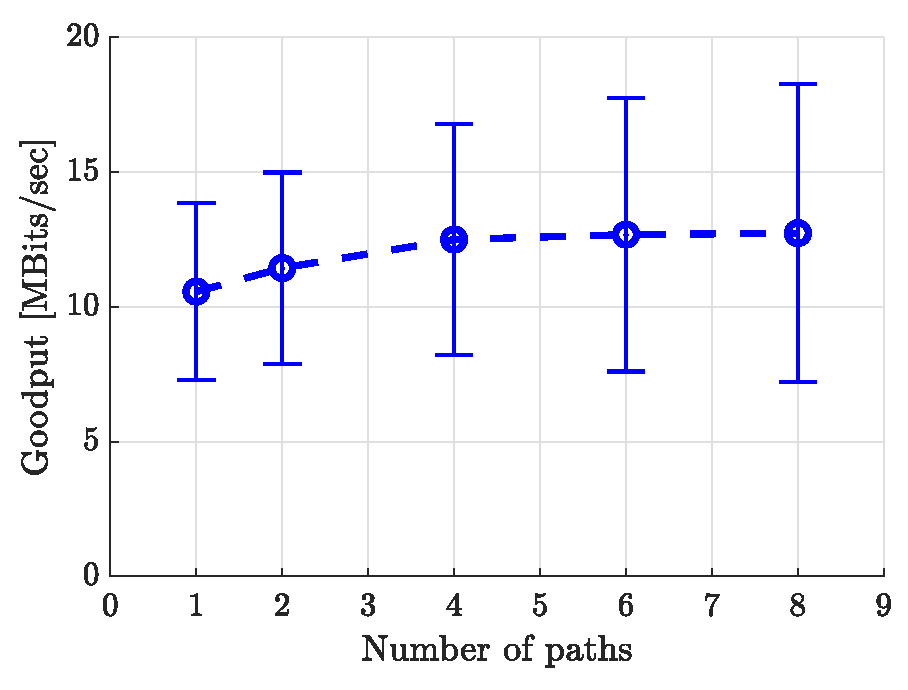
\includegraphics[scale=0.65]{../illustrations/performanceEvaluation/PerformanceWrtPathShortestpath.eps}  
		\caption[Caption for the list of figures.]{Plot of goodput depending on the number of paths used. An increasing number of paths leads to an increase in goodput. Path selection was done by minimizing the path length.}
		\label{fig:GoodputWrtToNOfPathsForShortestPath}
	\end{center}
\end{figure}

\subsection*{Influence of Path Selection}
\label{subsec:InfluencePathSelection}

Table \ref{tab:InfluenceOfPathSelection} shows the goodput obtained for the Shila Measurement for all three path selection criteria. The chosen criterion does not influence the achieved performance. Reasons for this can be found in the topology of the SCIONLab network. Table \ref{tab:DiffFromOptimal}  shows for each path selection algorithm the percentage deviation to the optimal value of the other metrics. The optimal value of a certain metric corresponds hereby to the value obtained by optimization with the corresponding path selection algorithm. 

\begin{table}
	\begin{center}
		\ra{1.3}
		\begin{tabular}{lcccccc}\toprule
			Paths & MTU & Path length & Sharability \\\midrule
			1  & 10.37 {\small $\pm$ 3.17} & 10.57 {\small $\pm$ 3.28} & 10.34 {\small $\pm$ 3.24} \\
			2  & 11.67 {\small $\pm$ 3.72} & 11.44 {\small $\pm$ 3.55} & 11.26 {\small $\pm$ 4.18} \\
			4  & 12.55 {\small $\pm$ 4.34} & 12.5  {\small $\pm$ 4.29} & 12.09 {\small $\pm$ 4.64} \\
			6  & 12.45 {\small $\pm$ 5.32} & 12.68 {\small $\pm$ 5.08} & 12.75 {\small $\pm$ 5.37} \\
			8  & 12.63 {\small $\pm$ 5.37} & 12.74 {\small $\pm$ 5.53} & 12.46 {\small $\pm$ 5.72} \\\bottomrule
		\end{tabular}
		\caption{Listing of the achieved goodput in MBits/sec for different numbers of paths and path selection criteria. The algorithm used for path selection does not influence performance.}
		\label{tab:InfluenceOfPathSelection}
	\end{center}
\end{table}

\begin{table}
	\begin{center}
		\ra{1.3}
		\begin{tabular}{lccc}\toprule
			   			Paths & MTU & Path length & Sharability \\\midrule
			
			{\footnotesize Path Selection: }MTU			& & & \\
			1  	& - & 0 & 0    \\
			2  	& - & 0 & 0.72 {\small $\pm$ 0.21}  \\
			4  	& - & 0 & 0.34 {\small $\pm$ 0.16} \\
			6  	& - & 0 & 0.12 {\small $\pm$ 0.08} \\
			8  	& - & 0 & 0.06 {\small $\pm$ 0.06} \smallskip\\
			{\footnotesize Path Selection: }Path length  	& & & \\
			1  	& 0 & - & 0    \\
			2  	& 0 & - & 0.72 {\small $\pm$ 0.21} \\
			4  	& 0 & - & 0.34 {\small $\pm$ 0.16} \\
			6  	& 0 & - & 0.06 {\small $\pm$ 0.05} \\
			8 		& 0 & - & 0.05 {\small $\pm$ 0.05} \smallskip\\
			{\footnotesize Path Selection: }Sharability		& & & \\
			1  	& 0 & 0    & - \\
			2 	& 0 & 0.21 {\small $\pm$ 0.10}  & - \\
			4  	& 0 & 0.21 {\small $\pm$ 0.07} & - \\
			6  	& 0 & 0.16 {\small $\pm$ 0.07} & - \\
			8  	& 0 & 0.16 {\small $\pm$  0.07} & - \\\bottomrule
		\end{tabular}
		\caption{Listing showing for each path selection the percentage deviation
			to the optimal value of the other metrics. Note that the Sharability for a single path is always zero. As an example of how to read the table: If the path selection is done using Sharability, the average length for two and four paths increases by 21\% compared to the optimal length. The optimal length is determined by the path selection using path length as an optimization criterion.}
		\label{tab:DiffFromOptimal}
	\end{center}
\end{table}

For all possible paths in the network, the same value for the MTU was obtained, irrespective of what metric for the selection was used. A possible positive effect of choosing paths with a higher MTU could therefore not be recognized at all. 

Comparing the average length of the paths, obtained when optimized for minimal path length and maximal MTU, no deviation is found. A possible negative effect of longer paths when using MTU instead of path length could therefore also not be observed. If we now bring the Sharability into play, we notice that an optimization by MTU or path length leads to a deterioration of the Sharability value. However, this has no negative impact on the goodput achieved. Such a negative effect could especially then be observed,  if bottlenecks in the network can be avoided by choosing the most different paths. If all shared links have sufficient capacity, this doesn't matter. We can therefore assume, that there were no capacity bottlenecks in the used links at the time the measurement was conducted. 

Concerning the Sharability values in Table \ref{tab:DiffFromOptimal}, two things are noteworthy:

The values for the two path selection criteria MTU and Path length are almost identical. It is conceivable that the same selection resulted from both path selection procedures\footnote{Remember, the MTU is identical for all paths in the network.}. The path selection mechanism of Shila itself does not implement an explicit tiebreaker. However, the paths received from the SCION infrastructure may be already sorted by a criterion, in this case the length.

It is furthermore noticeable that the deterioration of Sharability is particularly marked when using just a few paths. This can be explained by the topology of the network. There are only a limited number of truly distinct paths between two endpoints available. As long as this number is not exhausted, the Sharability can be kept very small, but can also be as large if a different metric for selection is chosen, hence the potential for deviation is large. Once all distinct paths are used up, additional paths have to include already used path segments, the optimal value cannot be that small anymore, reducing the potential for deviation.

Using the Sharability as path selection criterion leads on average to an increase in path length between 15\% and 20\%. In the Shila Measurement, this increase has no negative influence on the performance achieved. 

\subsection*{Comparison with QUIC}
\label{subsec:ComparisonWithQUIC}

Table \ref{tab:ComparisonWithQUIC} shows the values for goodput and throughput obtained from the Shila Measurement and the Quic Measurement. 

\subsubsection{Goodput}

Concerning goodput, QUIC over SCION outperforms Shila. Compared to MPTCP via SCION with a single path, QUIC achieves a goodput that is more than 3 times better. With the use of eight paths for MPTCP via SCION the performance is still more than 2.5 times better. The data exchange with MPTCP via SCION means a detour for the data in both endpoints. The individual segments travel via a virtual interface to the kernel, back to the userland application Shila and from there through SCION and its networking stack. Once at the destination, the same procedure is repeated in reverse order. These additional distances inevitably lead to an increase of the Round-Trip-Time which has a negative effect on the achieved goodput.

\subsubsection{Throughput}

About 33\%, i.e. a good third, of the total throughput of MPTCP over SCION is overhead. For QUIC over SCION it is only around 10\%, meaning that the the latter approach performs better in this category as well. 

\begin{table}[H]
	\begin{center}
		\ra{1.3}
		\begin{tabular}{lcccc}\toprule
			Paths & \multicolumn{2}{c}{Shila Measurement} & \multicolumn{2}{c}{Quic Measurement}
			\\\cmidrule(lr){2-3}\cmidrule(lr){4-5}
			& \small{Goodput}  & {\small Throughput} & \small{Goodput}  & {\small Throughput} \\\midrule
			1  & 10.75 {\small $\pm$ 3.28} & 17.45 {\small $\pm$ 5.91}  & 33.31 {\small $\pm$ 3.28} & 36.82 {\small $\pm$ 3.62} \\
			8  & 12.74 {\small $\pm$ 5.53} & 19.37 {\small $\pm$ 8.36}  & - & -		 \\\bottomrule
		\end{tabular}
		\caption{Comparison of goodput and throughput in MBits/sec between the Shila and Quic Measurement. For Shila, path selection was done by minimizing the path length.}
		\label{tab:ComparisonWithQUIC}
	\end{center}
\end{table}

\section{Conclusion}

Based on the results obtained, we can answer the questions asked at the beginning:

{\small \begin{enumerate}
	\item How does the performance behave in relation to the number of paths used for a connection? \smallskip\\ \textbf{Increasing the number of paths leads to better performance. In the measurements conducted an increase in average goodput up to 20\% could be observed.}
	\item How does the path selection algorithm influence performance?
	\smallskip\\ \textbf{Using different path selection algorithms does not influence performance. For the measurements carried out, none of the selection criteria was able to bypass a potential bottleneck in the network infrastructure and thus achieve better performance than the other criteria.}
	\item How well does Shila compare to QUIC over SCION?
	\smallskip\\ \textbf{QUIC over SCION outperforms MPTCP over SCION concerning goodput and overhead.}
\end{enumerate}}

Although the questions can be answered well based on the taken measurements, a final answer to the performance of Shila should not be drawn from them. Rather, these initial results should be used as the basis for further questions and improvements to Shila. In Chapter \ref{chap:FutureWork}, we discuss the questions that have emerged and possible improvements that can be addressed in future work.  
\chapter{Future Work}
\label{chap:FutureWork}

In this final chapter we discuss possible future work on the improvement and further development of Shila but also in general of MPTCP over SCION.

\section*{Further testing}

After completion of the implementation, we checked and ensured the basic functionality of Shila in simple tests both in local and SCIONLab infrastructure. However, during the execution of the Shila Measurement, presented in the previous chapter, individual experiments occasionally failed. Of course, such experiments were repeated and not included in the measurements. The exact reasons for the failure have not been investigated in the course of this work, but the failed experiments have all been documented. An important part of the revision and further development of Shila is to use this documentation to identify and fix possible weaknesses and bugs. Hereby the infrastructure \cite{} developed for the execution of the measurements can be optimally used to perform further extensive test runs.

\section*{More flexible Routing-Information}

In the current version of Shila, there is only one way to pass the Routing-Information, i.e. the mapping from TCP Address to SCION Address. The information has to be passed along with the startup of the shim layer. This assumes that the mapping is already known and means a restriction in flexibility.  

One possible solution was investigated in the conceptual phase of the thesis: The record route option of the IP protocol allows to log the route of a datagram through the Internet. When enabled, each IP datagram has space in its header to store up to eight IP addresses that it encounters on its way from sender to receiver. A predefined data structure has to be specified during the creation of the socket to activate this optional socket option. This structure describes the 32 bytes of memory required for storing the addresses and can instead of the usual zero also be initialized with the SCION target address. Each packet sent from the socket created with this option contains the SCION destination address in its IP header. The SCION target address for a new Main-Flow can then be extracted by Shila from the first intercepted datagram. With a wrapper around the standard TCP API, the process of additional address specification can be made pleasant for the user. Of the 32 bytes of the record route option, 28 bytes can be used effectively. The first four bytes are overwritten when traversing the virtual interface on the way to Shila. A SCION address requires a maximum of 20 bytes. With this approach its therefore possible to pass further control information, up eight bytes, from the application to Shila. At first glance, this approach has the disadvantage of increasing the overhead. But there is nothing to be said against reassembling the IP packet in Shila without the additional option. The stated approach is not yet part of the implementation since not strictly needed for the basic functionality. But once part of Shila, it increases the flexibility and possibilities of the shim layer.

\section*{Reducing overhead}

As we have seen in the previous chapter, the data exchange with MPTCP over SCION comes with comparatively high overhead. This is also due to the multiple nesting of the payload within a SCION packet: It contains a Shila-Message\footnote{A Shila-Message is the message sent between two Shila instances via the Backbone-Connection.}, which itself holds a TCP segment in an IP datagram. The actual data sits inside the TCP packet. In this nesting, information is sent along which does not necessarily have to be transmitted. It is not necessary to include the source and destination address in the IP header, these are clearly defined by the TCP flow of the backbone connection. The same applies to the protocol identification number or the checksum, which can be recalculated. An approach to reduce overhead would, therefore, be to go without the IP header but just the TCP segment as payload and a custom header. Such a header holds only the information required to reassemble the IP packet at the receiving endpoint. An IP header without additional options has a size of 20 bytes. The identification value (2 bytes) and the flags together with the fragment offset (2 bytes) must be included in the custom header for every IP datagram processed by Shila. The remaining information necessary for the re-composition of the IP packet at the destination endpoint can either be calculated, e.g. the checksum, or is given through to the backbone connection, e.g. source and destination address. With this approach, the contribution of the IP header to overhead can be reduced by 80\%. Redundant information is also sent in the TCP segment, the source and destination ports are also given by the backbone connection. But the savings potential for combining the TCP header is lower, the majority of the fields contain dynamic information. If the proposal under discussion is implemented, the additional effort for parsing and recompiling the IP datagrams should not be disregarded.

\section*{Shorter distances with XDP}

Interposing Shila between MPTCP and SCION inevitably increases the round-trip time and has a negative effect on throughput. Besides the computational effort within the shim layer, using Shila means for the data an additional loop through the kernel networking functionality in both endpoints, as illustrated on the left side of Figure \ref{fig:ShilaDetourKernel}. Its therefore desirable to shorten this additional detour in future work and therefore the improve the performance of Shila. A possible technology that could be used for this improvement is XDP.

\begin{figure}[H]
	\begin{center}
		\def\svgwidth{1\textwidth}
		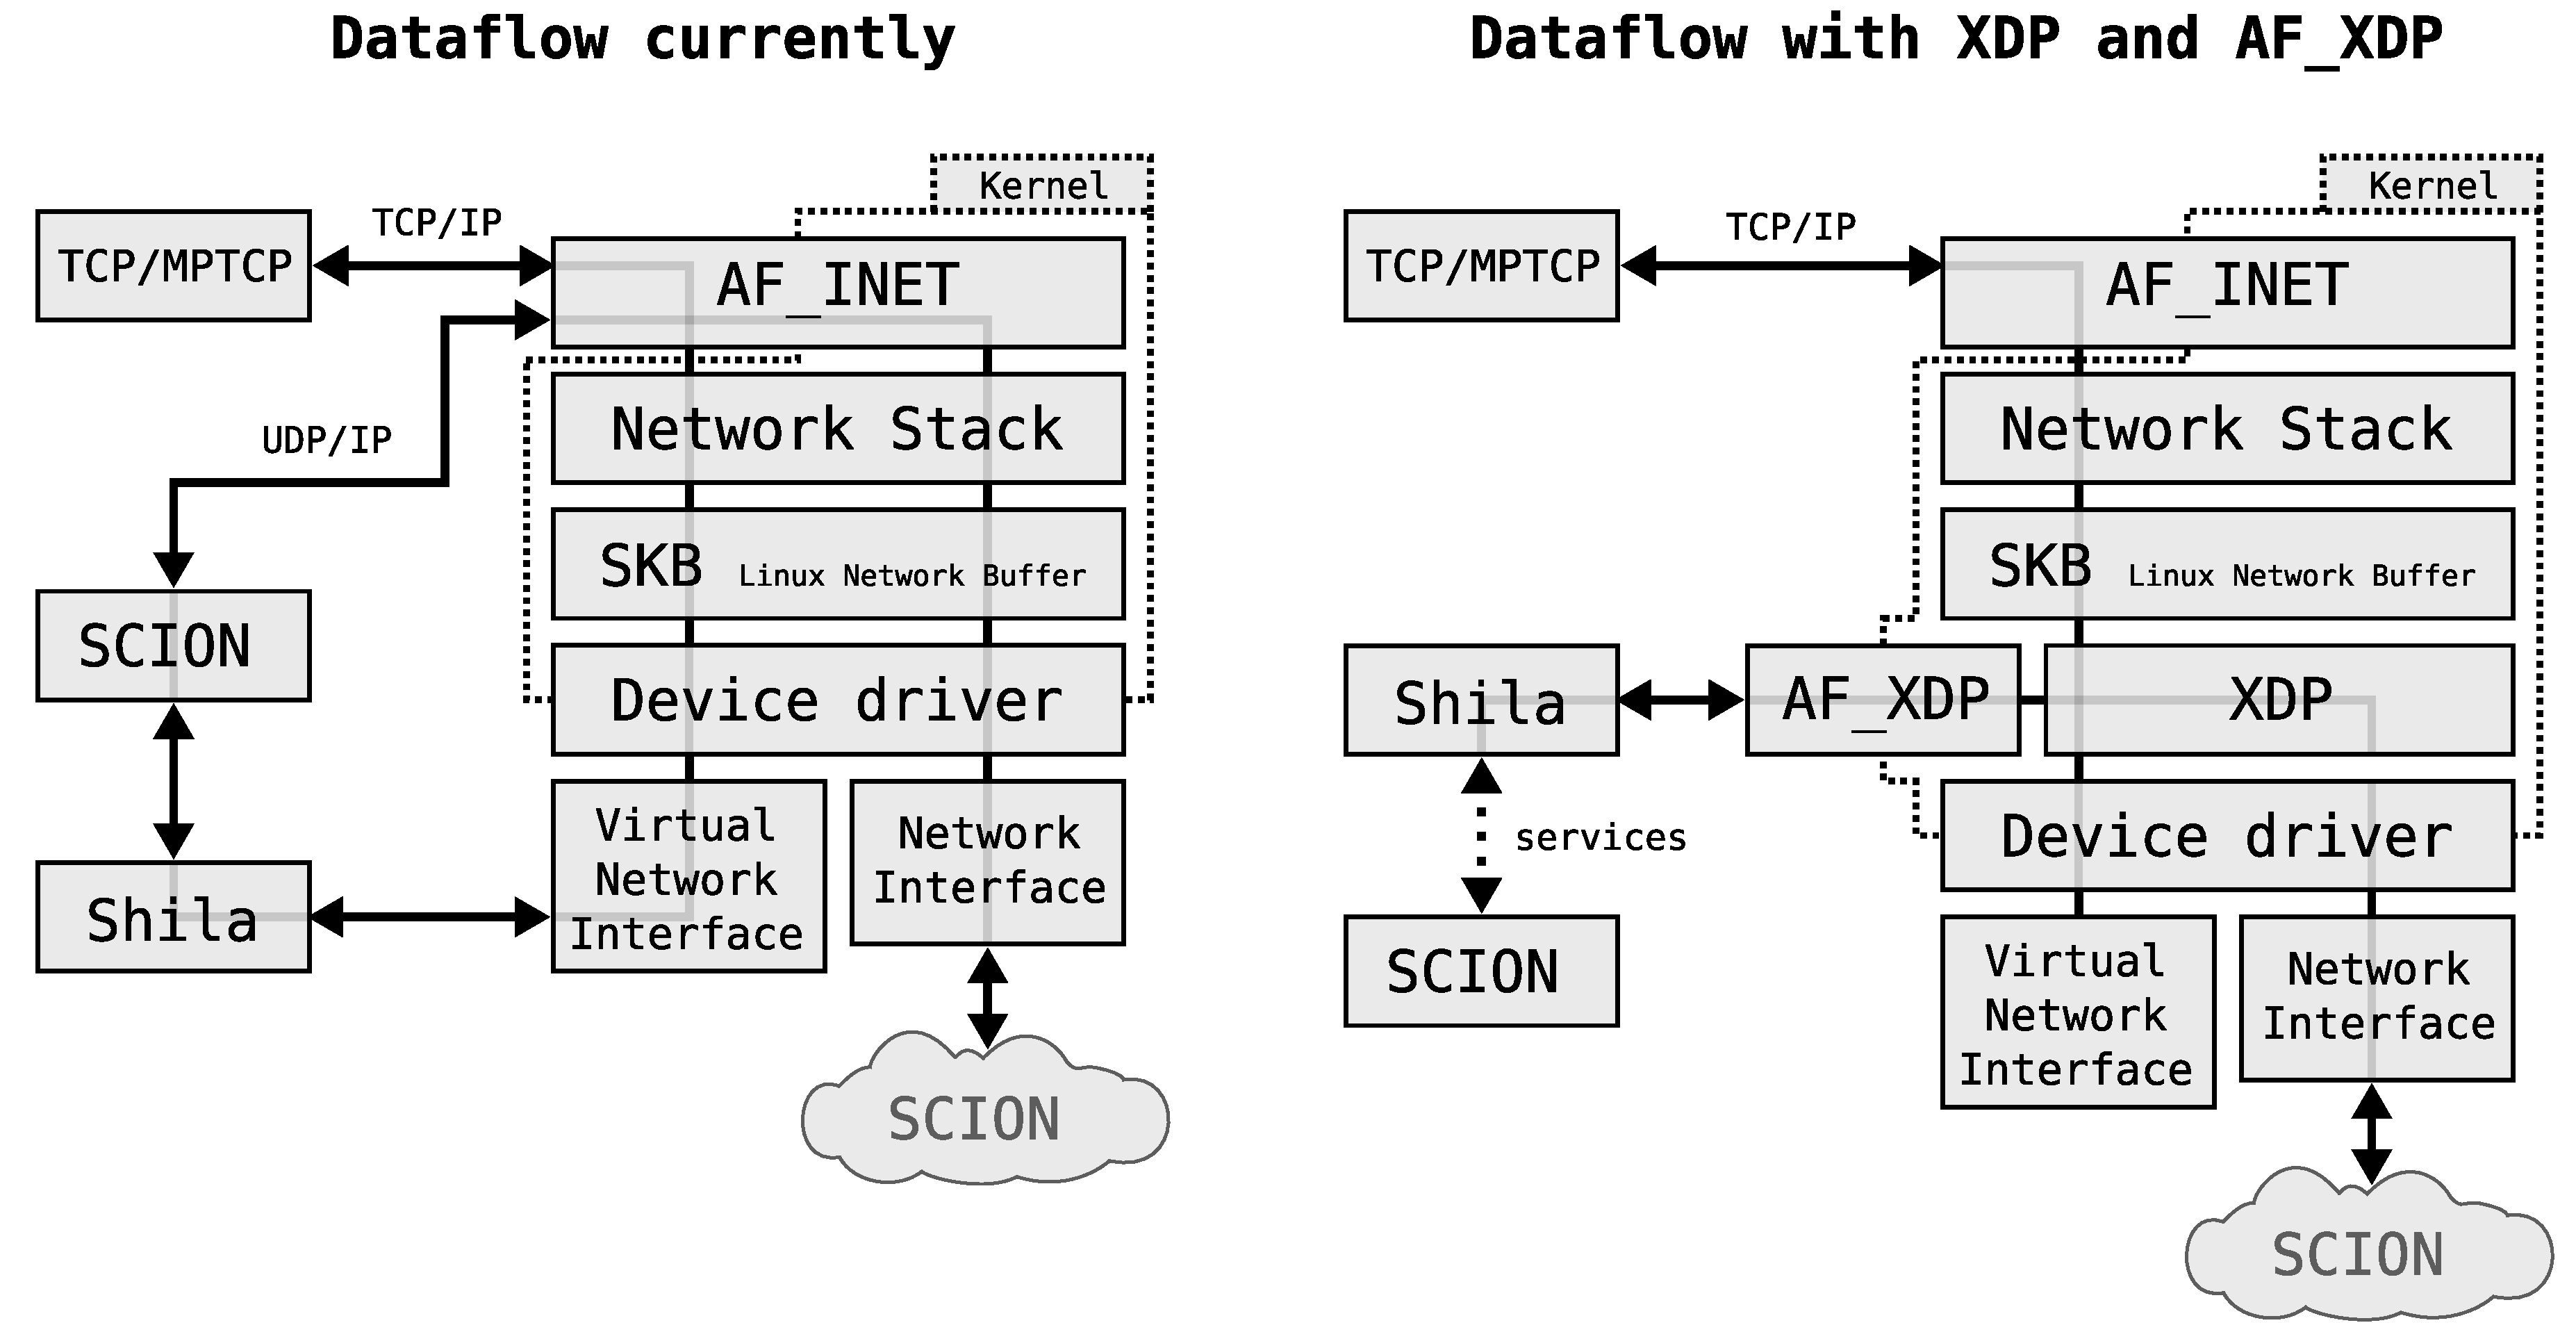
\includegraphics[scale=0.2]{../illustrations/futureWork/DetourAndWithXDP.pdf}   
		\caption[Caption for the list of figures.]{On the left side, the path taken by data exchanged via MPTCP over SCION is illustrated. In both endpoints, the kernel is traversed twice. The right side illustrates the path taken when using XDP (eXpress Data Path). This time the kernel is only traversed once per endpoint.}
		\label{fig:ShilaDetourKernel}
	\end{center}
\end{figure}

XDP \cite{XDP,XDPGitHub}, short for eXpress Data Path, is a relatively recent approach to programmable packet processing. It is not the first technology that allows the programmable processing of packets, but its approach differs from known solutions.  Known products like the  DataPlane Development Kit (DPDK) \cite{DPDK} bypass the kernel at all. The complete control of the network hardware is hand over to the networking application residing in user space. This comes with the advantage that the costs caused by the userland-kernel boundary can be avoided. But the approach also has disadvantages. By completely bypassing the kernel, useful functionalities of the network stack are not available, which complicates the implementation using these so-called kernel bypass approaches. Besides, are important security and isolation mechanisms of the kernel, ensuring the stability and security of the system, circumvented as well. 

In contrast, with XDP, programmable packet processing is integrated directly into the kernel. Even before the kernel handles an incoming packet, the so-called XDP driver hook is executed as part of the device driver. Within this customizable XDP program, there are various options for processing the packet. These include parsing, editing of header or payload or even the creation of additional metadata. Once the hook is done, it has again multiple options: It can either drop the packet, directly send it out via the receiving interface or to hand it over to the networking stack. As a fourth option, the packet can be redirected to different destinations, one of them is called AF\_XDP. AF\_XDP \cite{AFXDPPaper, AFXDPWeb,AFXDPWeb2} is a special socket type that allows the exchange of raw packets between the network interface and a userland application at a high speed. In addition to AF\_XDP, the XDP driver hook can use another process or network interface as further destinations for forwarding the packet.

With the help of XDP and AF\_XDP, the double way through the kernel can be saved. The shortened path of the data is illustrated in Figure \ref{fig:ShilaDetourKernel} on the right.  Packets sent from the TCP/MPTCP instance towards the virtual interface can be redirected to Shila using a corresponding XDP hook\footnote{XDP provides mechanisms to redirect outgoing traffic as well.}. Shila reads the IP datagrams from the AF\_XDP socket, extracts the necessary data and creates a SCION packet. This packet is then sent over the SCION network via the AF\_XDP socket of the outgoing network interface. On the receiving side, the same procedure is performed in reverse order. Shila unpacks the received SCION packet and creates the IP datagram which is then pushed through the network stack towards the receiving TCP/MPTCP instance.

Even if the proposed alternative is promising, the effort of implementation should not be underestimated. Since relatively new, the technology is constantly being revised and developed, occasional changes to the API must be expected. Furthermore requires XDP support from the network interface drivers to fully unfold its potential. Something which makes, at least at the moment, the usage of this technology less attractive. When approaching the implementation it should be taken into account that a part or maybe even the whole functionality of Shila, e.g. the parsing of the packets, can be integrated into an XDP. As already mentioned, the technology is constantly being developed and its functionality is being expanded. It is therefore desirable to investigate how far this integration is feasible, to maybe even save the way back into the userland.  
	
\section{Namespace less solution}

\section{Further measurements}

\section{Avoidance of appnet}

\section{Path Selection}


\chapter{Conclusion}
\label{chap:Conclusion}

With the presented implementation of Shila, a shim layer between MPTCP and SCION, the combined use of the two promising technologies becomes possible. TCP applications can now be operated over SCION without any changes being necessary. If the endpoints furthermore support MPTCP, the applications also benefit from the advantages of using multiple paths orchestrated by MPTCP and inherently supported by SCION. With its prototype character, the implementation of Shila does not achieve the same performance as comparable approaches yet. However, with the development and improvement options we have identified for Shila, we were able to illustrate the potential of this approach and provide the groundwork for future research dedicated to close the performance gap. Even if it is only a tiny piece of the mosaic in SCION's ultimate goal: We are pleased with the contribution made in developing Shila, our own little heroine, for a more reliable, fairer and safer internet.

%\appendix

%\input{appendix}

\backmatter

\bibliographystyle{plain}
\bibliography{refs}

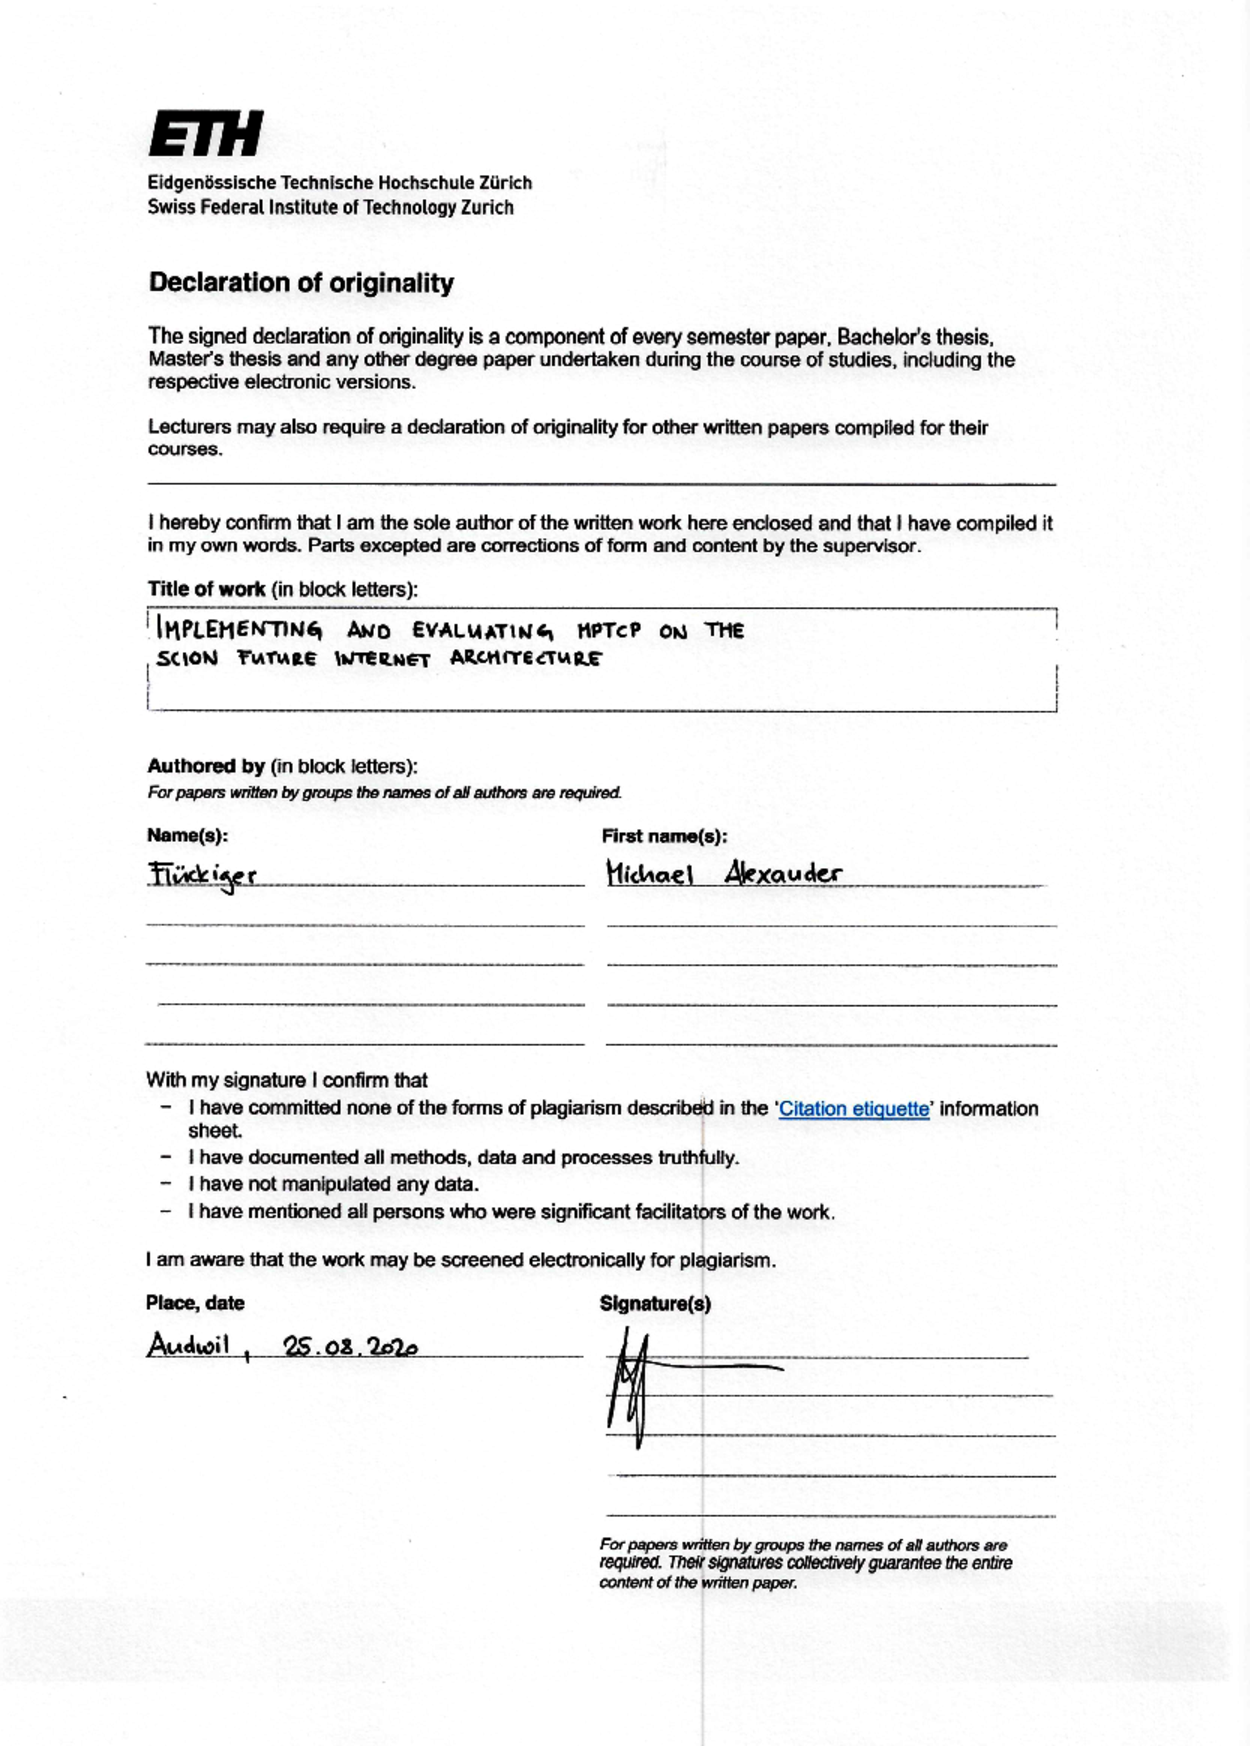
\includepdf[pages={-}]{../declaration-originality.pdf}

\end{document}
